%% bare_jrnl.tex
%% V1.4a
%% 2014/09/17
%% by Michael Shell
%% see http://www.michaelshell.org/
%% for current contact information.
%%
%% This is a skeleton file demonstrating the use of IEEEtran.cls
%% (requires IEEEtran.cls version 1.8a or later) with an IEEE
%% journal paper.
%%
%% Support sites:
%% http://www.michaelshell.org/tex/ieeetran/
%% http://www.ctan.org/tex-archive/macros/latex/contrib/IEEEtran/
%% and
%% http://www.ieee.org/

%%*************************************************************************
%% Legal Notice:
%% This code is offered as-is without any warranty either expressed or
%% implied; without even the implied warranty of MERCHANTABILITY or
%% FITNESS FOR A PARTICULAR PURPOSE!
%% User assumes all risk.
%% In no event shall IEEE or any contributor to this code be liable for
%% any damages or losses, including, but not limited to, incidental,
%% consequential, or any other damages, resulting from the use or misuse
%% of any information contained here.
%%
%% All comments are the opinions of their respective authors and are not
%% necessarily endorsed by the IEEE.
%%
%% This work is distributed under the LaTeX Project Public License (LPPL)
%% ( http://www.latex-project.org/ ) version 1.3, and may be freely used,
%% distributed and modified. A copy of the LPPL, version 1.3, is included
%% in the base LaTeX documentation of all distributions of LaTeX released
%% 2003/12/01 or later.
%% Retain all contribution notices and credits.
%% ** Modified files should be clearly indicated as such, including  **
%% ** renaming them and changing author support contact information. **
%%
%% File list of work: IEEEtran.cls, IEEEtran_HOWTO.pdf, bare_adv.tex,
%%                    bare_conf.tex, bare_jrnl.tex, bare_conf_compsoc.tex,
%%                    bare_jrnl_compsoc.tex, bare_jrnl_transmag.tex
%%*************************************************************************


% *** Authors should verify (and, if needed, correct) their LaTeX system  ***
% *** with the testflow diagnostic prior to trusting their LaTeX platform ***
% *** with production work. IEEE's font choices and paper sizes can       ***
% *** trigger bugs that do not appear when using other class files.       ***                          ***
% The testflow support page is at:
% http://www.michaelshell.org/tex/testflow/



\documentclass[journal]{IEEEtran}
%
% If IEEEtran.cls has not been installed into the LaTeX system files,
% manually specify the path to it like:
% \documentclass[journal]{../sty/IEEEtran}





% Some very useful LaTeX packages include:
% (uncomment the ones you want to load)


% *** MISC UTILITY PACKAGES ***
%
%\usepackage{ifpdf}
% Heiko Oberdiek's ifpdf.sty is very useful if you need conditional
% compilation based on whether the output is pdf or dvi.
% usage:
% \ifpdf
%   % pdf code
% \else
%   % dvi code
% \fi
% The latest version of ifpdf.sty can be obtained from:
% http://www.ctan.org/tex-archive/macros/latex/contrib/oberdiek/
% Also, note that IEEEtran.cls V1.7 and later provides a builtin
% \ifCLASSINFOpdf conditional that works the same way.
% When switching from latex to pdflatex and vice-versa, the compiler may
% have to be run twice to clear warning/error messages.






% *** CITATION PACKAGES ***
%
%\usepackage{cite}
% cite.sty was written by Donald Arseneau
% V1.6 and later of IEEEtran pre-defines the format of the cite.sty package
% \cite{} output to follow that of IEEE. Loading the cite package will
% result in citation numbers being automatically sorted and properly
% "compressed/ranged". e.g., [1], [9], [2], [7], [5], [6] without using
% cite.sty will become [1], [2], [5]--[7], [9] using cite.sty. cite.sty's
% \cite will automatically add leading space, if needed. Use cite.sty's
% noadjust option (cite.sty V3.8 and later) if you want to turn this off
% such as if a citation ever needs to be enclosed in parenthesis.
% cite.sty is already installed on most LaTeX systems. Be sure and use
% version 5.0 (2009-03-20) and later if using hyperref.sty.
% The latest version can be obtained at:
% http://www.ctan.org/tex-archive/macros/latex/contrib/cite/
% The documentation is contained in the cite.sty file itself.

\usepackage{graphicx}
\usepackage{color}
\usepackage{tabularray}
\usepackage{adjustbox}
\usepackage{listings}
\usepackage{xcolor}
\usepackage{hyperref}
\usepackage{subcaption}
\usepackage{threeparttable}
\usepackage{multirow}

%\hypersetup{
%  colorlinks=true,
%  urlcolor=blue,
%}

%New colors defined below
\definecolor{dotgreen}{RGB}{0,176,80}
\definecolor{dotsky}{RGB}{0,176,240}
\definecolor{dotred}{RGB}{192,0,0}

% Bibliography settings
\usepackage[style=ieee]{biblatex}
\addbibresource{references.bib}

% Linea de referencias de pie de página
\renewcommand{\footnoterule}
 {\noindent\smash{\rule[3pt]{0.5\textwidth}{0.4pt}}}


% *** GRAPHICS RELATED PACKAGES ***
%
\ifCLASSINFOpdf
  % \usepackage[pdftex]{graphicx}
  % declare the path(s) where your graphic files are
  % \graphicspath{{../pdf/}{../jpeg/}}
  % and their extensions so you won't have to specify these with
  % every instance of \includegraphics
  % \DeclareGraphicsExtensions{.pdf,.jpeg,.png}
\else
  % or other class option (dvipsone, dvipdf, if not using dvips). graphicx
  % will default to the driver specified in the system graphics.cfg if no
  % driver is specified.
  % \usepackage[dvips]{graphicx}
  % declare the path(s) where your graphic files are
  % \graphicspath{{../eps/}}
  % and their extensions so you won't have to specify these with
  % every instance of \includegraphics
  % \DeclareGraphicsExtensions{.eps}
\fi
% graphicx was written by David Carlisle and Sebastian Rahtz. It is
% required if you want graphics, photos, etc. graphicx.sty is already
% installed on most LaTeX systems. The latest version and documentation
% can be obtained at:
% http://www.ctan.org/tex-archive/macros/latex/required/graphics/
% Another good source of documentation is "Using Imported Graphics in
% LaTeX2e" by Keith Reckdahl which can be found at:
% http://www.ctan.org/tex-archive/info/epslatex/
%
% latex, and pdflatex in dvi mode, support graphics in encapsulated
% postscript (.eps) format. pdflatex in pdf mode supports graphics
% in .pdf, .jpeg, .png and .mps (metapost) formats. Users should ensure
% that all non-photo figures use a vector format (.eps, .pdf, .mps) and
% not a bitmapped formats (.jpeg, .png). IEEE frowns on bitmapped formats
% which can result in "jaggedy"/blurry rendering of lines and letters as
% well as large increases in file sizes.
%
% You can find documentation about the pdfTeX application at:
% http://www.tug.org/applications/pdftex





% *** MATH PACKAGES ***
%
%\usepackage[cmex10]{amsmath}
% A popular package from the American Mathematical Society that provides
% many useful and powerful commands for dealing with mathematics. If using
% it, be sure to load this package with the cmex10 option to ensure that
% only type 1 fonts will utilized at all point sizes. Without this option,
% it is possible that some math symbols, particularly those within
% footnotes, will be rendered in bitmap form which will result in a
% document that can not be IEEE Xplore compliant!
%
% Also, note that the amsmath package sets \interdisplaylinepenalty to 10000
% thus preventing page breaks from occurring within multiline equations. Use:
%\interdisplaylinepenalty=2500
% after loading amsmath to restore such page breaks as IEEEtran.cls normally
% does. amsmath.sty is already installed on most LaTeX systems. The latest
% version and documentation can be obtained at:
% http://www.ctan.org/tex-archive/macros/latex/required/amslatex/math/





% *** SPECIALIZED LIST PACKAGES ***
%
%\usepackage{algorithmic}
% algorithmic.sty was written by Peter Williams and Rogerio Brito.
% This package provides an algorithmic environment fo describing algorithms.
% You can use the algorithmic environment in-text or within a figure
% environment to provide for a floating algorithm. Do NOT use the algorithm
% floating environment provided by algorithm.sty (by the same authors) or
% algorithm2e.sty (by Christophe Fiorio) as IEEE does not use dedicated
% algorithm float types and packages that provide these will not provide
% correct IEEE style captions. The latest version and documentation of
% algorithmic.sty can be obtained at:
% http://www.ctan.org/tex-archive/macros/latex/contrib/algorithms/
% There is also a support site at:
% http://algorithms.berlios.de/index.html
% Also of interest may be the (relatively newer and more customizable)
% algorithmicx.sty package by Szasz Janos:
% http://www.ctan.org/tex-archive/macros/latex/contrib/algorithmicx/




% *** ALIGNMENT PACKAGES ***
%
%\usepackage{array}
% Frank Mittelbach's and David Carlisle's array.sty patches and improves
% the standard LaTeX2e array and tabular environments to provide better
% appearance and additional user controls. As the default LaTeX2e table
% generation code is lacking to the point of almost being broken with
% respect to the quality of the end results, all users are strongly
% advised to use an enhanced (at the very least that provided by array.sty)
% set of table tools. array.sty is already installed on most systems. The
% latest version and documentation can be obtained at:
% http://www.ctan.org/tex-archive/macros/latex/required/tools/


% IEEEtran contains the IEEEeqnarray family of commands that can be used to
% generate multiline equations as well as matrices, tables, etc., of high
% quality.




% *** SUBFIGURE PACKAGES ***
%\ifCLASSOPTIONcompsoc
%  \usepackage[caption=false,font=normalsize,labelfont=sf,textfont=sf]{subfig}
%\else
%  \usepackage[caption=false,font=footnotesize]{subfig}
%\fi
% subfig.sty, written by Steven Douglas Cochran, is the modern replacement
% for subfigure.sty, the latter of which is no longer maintained and is
% incompatible with some LaTeX packages including fixltx2e. However,
% subfig.sty requires and automatically loads Axel Sommerfeldt's caption.sty
% which will override IEEEtran.cls' handling of captions and this will result
% in non-IEEE style figure/table captions. To prevent this problem, be sure
% and invoke subfig.sty's "caption=false" package option (available since
% subfig.sty version 1.3, 2005/06/28) as this is will preserve IEEEtran.cls
% handling of captions.
% Note that the Computer Society format requires a larger sans serif font
% than the serif footnote size font used in traditional IEEE formatting
% and thus the need to invoke different subfig.sty package options depending
% on whether compsoc mode has been enabled.
%
% The latest version and documentation of subfig.sty can be obtained at:
% http://www.ctan.org/tex-archive/macros/latex/contrib/subfig/




% *** FLOAT PACKAGES ***
%
%\usepackage{fixltx2e}
% fixltx2e, the successor to the earlier fix2col.sty, was written by
% Frank Mittelbach and David Carlisle. This package corrects a few problems
% in the LaTeX2e kernel, the most notable of which is that in current
% LaTeX2e releases, the ordering of single and double column floats is not
% guaranteed to be preserved. Thus, an unpatched LaTeX2e can allow a
% single column figure to be placed prior to an earlier double column
% figure. The latest version and documentation can be found at:
% http://www.ctan.org/tex-archive/macros/latex/base/


%\usepackage{stfloats}
% stfloats.sty was written by Sigitas Tolusis. This package gives LaTeX2e
% the ability to do double column floats at the bottom of the page as well
% as the top. (e.g., "\begin{figure*}[!b]" is not normally possible in
% LaTeX2e). It also provides a command:
%\fnbelowfloat
% to enable the placement of footnotes below bottom floats (the standard
% LaTeX2e kernel puts them above bottom floats). This is an invasive package
% which rewrites many portions of the LaTeX2e float routines. It may not work
% with other packages that modify the LaTeX2e float routines. The latest
% version and documentation can be obtained at:
% http://www.ctan.org/tex-archive/macros/latex/contrib/sttools/
% Do not use the stfloats baselinefloat ability as IEEE does not allow
% \baselineskip to stretch. Authors submitting work to the IEEE should note
% that IEEE rarely uses double column equations and that authors should try
% to avoid such use. Do not be tempted to use the cuted.sty or midfloat.sty
% packages (also by Sigitas Tolusis) as IEEE does not format its papers in
% such ways.
% Do not attempt to use stfloats with fixltx2e as they are incompatible.
% Instead, use Morten Hogholm'a dblfloatfix which combines the features
% of both fixltx2e and stfloats:
%
% \usepackage{dblfloatfix}
% The latest version can be found at:
% http://www.ctan.org/tex-archive/macros/latex/contrib/dblfloatfix/




%\ifCLASSOPTIONcaptionsoff
%  \usepackage[nomarkers]{endfloat}
% \let\MYoriglatexcaption\caption
% \renewcommand{\caption}[2][\relax]{\MYoriglatexcaption[#2]{#2}}
%\fi
% endfloat.sty was written by James Darrell McCauley, Jeff Goldberg and
% Axel Sommerfeldt. This package may be useful when used in conjunction with
% IEEEtran.cls'  captionsoff option. Some IEEE journals/societies require that
% submissions have lists of figures/tables at the end of the paper and that
% figures/tables without any captions are placed on a page by themselves at
% the end of the document. If needed, the draftcls IEEEtran class option or
% \CLASSINPUTbaselinestretch interface can be used to increase the line
% spacing as well. Be sure and use the nomarkers option of endfloat to
% prevent endfloat from "marking" where the figures would have been placed
% in the text. The two hack lines of code above are a slight modification of
% that suggested by in the endfloat docs (section 8.4.1) to ensure that
% the full captions always appear in the list of figures/tables - even if
% the user used the short optional argument of \caption[]{}.
% IEEE papers do not typically make use of \caption[]'s optional argument,
% so this should not be an issue. A similar trick can be used to disable
% captions of packages such as subfig.sty that lack options to turn off
% the subcaptions:
% For subfig.sty:
% \let\MYorigsubfloat\subfloat
% \renewcommand{\subfloat}[2][\relax]{\MYorigsubfloat[]{#2}}
% However, the above trick will not work if both optional arguments of
% the \subfloat command are used. Furthermore, there needs to be a
% description of each subfigure *somewhere* and endfloat does not add
% subfigure captions to its list of figures. Thus, the best approach is to
% avoid the use of subfigure captions (many IEEE journals avoid them anyway)
% and instead reference/explain all the subfigures within the main caption.
% The latest version of endfloat.sty and its documentation can obtained at:
% http://www.ctan.org/tex-archive/macros/latex/contrib/endfloat/
%
% The IEEEtran \ifCLASSOPTIONcaptionsoff conditional can also be used
% later in the document, say, to conditionally put the References on a
% page by themselves.




% *** PDF, URL AND HYPERLINK PACKAGES ***
%
%\usepackage{url}
% url.sty was written by Donald Arseneau. It provides better support for
% handling and breaking URLs. url.sty is already installed on most LaTeX
% systems. The latest version and documentation can be obtained at:
% http://www.ctan.org/tex-archive/macros/latex/contrib/url/
% Basically, \url{my_url_here}.




% *** Do not adjust lengths that control margins, column widths, etc. ***
% *** Do not use packages that alter fonts (such as pslatex).         ***
% There should be no need to do such things with IEEEtran.cls V1.6 and later.
% (Unless specifically asked to do so by the journal or conference you plan
% to submit to, of course. )


% correct bad hyphenation here
\hyphenation{op-tical net-works semi-conduc-tor}


\begin{document}
%
% paper title
% Titles are generally capitalized except for words such as a, an, and, as,
% at, but, by, for, in, nor, of, on, or, the, to and up, which are usually
% not capitalized unless they are the first or last word of the title.
% Linebreaks \\ can be used within to get better formatting as desired.
% Do not put math or special symbols in the title.
\title{Data augmentation techniques applied to the classification of multi-station seismic-volcanic signals}
%
%
% author names and IEEE memberships
% note positions of commas and nonbreaking spaces ( ~ ) LaTeX will not break
% a structure at a ~ so this keeps an author's name from being broken across
% two lines.
% use \thanks{} to gain access to the first footnote area
% a separate \thanks must be used for each paragraph as LaTeX2e's \thanks
% was not built to handle multiple paragraphs
%

\author{Franz~Yupanqui~Machaca\textsuperscript{a,b,c}, Pablo~Salazar~Reinoso\textsuperscript{b,d}, and
  Claudio~Meneses~Villegas\textsuperscript{e}\\
  \vspace{1mm}
  \begin{flushleft}
  \small\textsuperscript{a}PhD in Sustainable Engineering, Universidad Católica del Norte, \iffalse Avenida Angamos 0610, 1270709 \fi Antofagasta, Chile\\
  \textsuperscript{b}Millennium Institute on Volcanic Risk Research – Ckelar Volcanoes, \iffalse Avenida Angamos 0610, 1270709 \fi Antofagasta, Chile\\
  \textsuperscript{c}4D Perceptio, La Paz, Bolivia\\
  \textsuperscript{d}Department of Geological Sciences, Universidad Católica del Norte, \iffalse Avenida Angamos 0610, 1270709 \fi Antofagasta, Chile\\
  \textsuperscript{e}Department of Computing and Systems Engineering, Universidad Católica del Norte, \iffalse Avenida Angamos 0610, 1270709 \fi Antofagasta, Chile\\
  \end{flushleft}
  \thanks{F. Yupanqui Machaca, \color{blue}\href{mailto:frayup@gmail.com}{frayup@gmail.com} }
  \thanks{C. Meneses Villegas, \color{blue}\href{mailto:cmeneses@ucn.cl}{cmeneses@ucn.cl} }
  \thanks{P. Salazar Reinoso, \color{blue}\href{mailto:pasalaz@ucn.cl}{pasalaz@ucn.cl} }
  %\thanks{Manuscript received April 19, 2005; revised September 17, 2025.}
}


% note the % following the last \IEEEmembership and also \thanks -
% these prevent an unwanted space from occurring between the last author name
% and the end of the author line. i.e., if you had this:
%
% \author{....lastname \thanks{...} \thanks{...} }
%                     ^------------^------------^----Do not want these spaces!
%
% a space would be appended to the last name and could cause every name on that
% line to be shifted left slightly. This is one of those "LaTeX things". For
% instance, "\textbf{A} \textbf{B}" will typeset as "A B" not "AB". To get
% "AB" then you have to do: "\textbf{A}\textbf{B}"
% \thanks is no different in this regard, so shield the last } of each \thanks
% that ends a line with a % and do not let a space in before the next \thanks.
% Spaces after \IEEEmembership other than the last one are OK (and needed) as
% you are supposed to have spaces between the names. For what it is worth,
% this is a minor point as most people would not even notice if the said evil
% space somehow managed to creep in.



% The paper headers
%\markboth{Journal of \LaTeX\ Class Files,~Vol.~13, No.~9, September~2025}
%{Shell \MakeLowercase{\textit{et al.}}: Bare Demo of IEEEtran.cls for Journals}
% The only time the second header will appear is for the odd numbered pages
% after the title page when using the twoside option.
%
% *** Note that you probably will NOT want to include the author's ***
% *** name in the headers of peer review papers.                   ***
% You can use \ifCLASSOPTIONpeerreview for conditional compilation here if
% you desire.




% If you want to put a publisher's ID mark on the page you can do it like
% this:
%\IEEEpubid{0000--0000/00\$00.00~\copyright~2014 IEEE}
% Remember, if you use this you must call \IEEEpubidadjcol in the second
% column for its text to clear the IEEEpubid mark.



% use for special paper notices
%\IEEEspecialpapernotice{(Invited Paper)}




% make the title area
\maketitle

% As a general rule, do not put math, special symbols or citations
% in the abstract or keywords.
\begin{abstract}
This paper presents and implements different data augmentation techniques applied to volcanic seismic signals. 
The datasets generated considered two types of data: real and augmented data that balance the original dataset, 
and datasets with fully augmented data. Using the datasets generated by these data augmentation techniques, 
volcanic seismic event classification models were trained in order to identify the data augmentation technique 
that generates the best performing models. In addition, by applying similarity and diversity metrics to the data 
generated by the data augmentation techniques, these characteristics were analysed in the different datasets.
\end{abstract}

% Note that keywords are not normally used for peerreview papers.
\begin{IEEEkeywords}
Deep Learning, Transfer Learning, Data Augmentation, Machine learning classification, Seismic volcanic signals, FID, KID, MS-SSIM.
\end{IEEEkeywords}






% For peer review papers, you can put extra information on the cover
% page as needed:
% \ifCLASSOPTIONpeerreview
% \begin{center} \bfseries EDICS Category: 3-BBND \end{center}
% \fi
%
% For peerreview papers, this IEEEtran command inserts a page break and
% creates the second title. It will be ignored for other modes.
\IEEEpeerreviewmaketitle



\section{Introduction}\label{introduction}
% The very first letter is a 2 line initial drop letter followed
% by the rest of the first word in caps.
%
% form to use if the first word consists of a single letter:
% \IEEEPARstart{A}{demo} file is ....
%
% form to use if you need the single drop letter followed by
% normal text (unknown if ever used by IEEE):
% \IEEEPARstart{A}{}demo file is ....
%
% Some journals put the first two words in caps:
% \IEEEPARstart{T}{his demo} file is ....
%
% Here we have the typical use of a "T" for an initial drop letter
% and "HIS" in caps to complete the first word.
%\IEEEPARstart{T}{his} demo file is intended to serve as a ``starter file''
% for IEEE journal papers produced under \LaTeX\ using IEEEtran.cls version 1.8a and later.
% You must have at least 2 lines in the paragraph with the drop letter
% (should never be an issue)
%I wish you the best of success.
%\hfill mds
%\hfill September 17, 2025

\subsection{The problem of recognition}
The signatures are not dangerous; however, volcanic and seismic events may be dangerous events that occur unexpectedly, although they present some signals before they occur. Globally, these events are continuously registered using seismometers. Afterward, expert geophysicists classify these data.\\
Seismic-volcanic activity has been studied for many years. Currently, this type of activity is registered by sensors that record signals in three dimensions. The seismic-volcanic pat- tern recognition process is typically done manually, although there are state-of-the-art studies that make the process in a semi-automatic o automatic form \cite{salazar2022multi,salazar2020deep,malfante2018automatic,bicego2012classification,curilem2016pattern, lara2020automatic}. These studies regularly consider one of the three available channels, one of several stations, and one volcano. In this context, classical machine learning (ML) and deep learning (DL) algorithms applied to the automatic classification of seismic-volcanic signatures are becoming an emerging research field to overcome the limitations of manual classification.\\
This study proposes and applies a series of data augmentation (DA) techniques to volcanic seismic events and analyzes their impact on the performance of event classification models. A database of events collected from the Láscar volcano over  an 8-month period and labelled by CKELAR-VOLCANES experts was considered. Five classes (see Table \ref{table:lascar_database}) were included according to the classification given by CKELAR-VOLCANES; see also \cite{salazar2022multi}. Given the nature of the seismic phenomena that occur in and around the volcano, the database is unbalanced, requiring a data balancing technique; therefore, DA techniques were considered. DA techniques were applied to generate two types of datasets: real and augmented data that balance the dataset and datasets with fully augmented data. Similarity and diversity metrics were applied to the data generated by the DA techniques to analyze these characteristics. Classification models were trained using DL and Transfer Learning (TL) techniques. The models were evaluated using precision, accuracy, recall, F1 score, and confusion matrix metrics. \\
Each seismic event is represented by its respective spectrogram, so that these images can be processed. Using the Transfer Learning strategy, event classification models were trained, considering the pre-trained AlexNet deep artificial neural network. Event classification models are trained on different datasets generated by different Data Augmentation techniques, and their performance is reviewed. \\
The results of the experiments are presented in terms of performance metrics, comparing the impact of each data augmentation method on the classification of seismic-volcanic events. The evaluation included models trained on real and augmented data, as well as models trained on entirely augmented datasets. The influence of similarity and diversity metrics on model generalization was also analyzed.\\
The remainder of this paper is organized as follows. The most recent bibliography on this subject is presented in Section \ref{literaturereview}. Section \ref{methodology} presents the methodology. The methods used are described in Section \ref{methods}. The main results are presented in Section \ref{results}. Section \ref{discussion} discusses the results of this study, and conclusions are presented in Section \ref{conclusion}.

\section{Literature review}\label{literaturereview}
\begin{table*}
\caption{Current status of seismic-volcanic signal classification studies.} % title of Table
\centering
\begin{adjustbox}{width=\textwidth}
\begin{tblr}{
  column{even} = {c},
  column{3} = {c},
  column{5} = {c},
  column{7} = {c},
}
\hline\hline %inserts double horizontal lines
Models and presentation year & Volcano - Country & Examples & Spectrogram & Channels & Stations & Classes & Accuracy
  (\%)\\
\hline
Hidden-Markov-Model-Based FSE(2013)\cite{bicego2012classification} & Galeras – Colombia & 300 & No & – & 2 & 3 & 96\\
Hidden-Markov-Model-Based FSE(2013)\cite{bicego2012classification} & Galeras – Colombia & 400 & No & – & 2 & 4 & 85.2\\
Topic Model (VT, LP, TR)(2015)\cite{bicego2015volcano} & Galeras – Colombia & 300 & No & – & 1 & 3 & 94.1\\
Topic Model (VT, LP, TR, HB)(2015)\cite{bicego2015volcano} & Galeras – Colombia & 400 & No & – & 1 & 4 & 83.8\\
Bag-of-Words (VT, LP, TR)(2015)\cite{bicego2015volcano} & Galeras – Colombia & 300 & No & – & 1 & 3 & 91.9\\
Bag-of-Words (VT, LP, TR, HB)(2015)\cite{bicego2015volcano} & Galeras – Colombia & 400 & No & – & 1 & 4 & 81.8\\
Support Vector Machines(2018)\cite{malfante2018automatic} & Ubinas – Perú & 109,609 & No & – & 1 & 6 & 93.5±0.5\\
CNN LeCun(2018)\cite{curilem2018using} & Llaima – Chile & 15,895 & Yes & – & 1 & 4 & 97.0\\
GRU-RNN y LFB(2018)\cite{titos2018detection} & Isla Decepción – Antártida & 2,193 & No & – & 1 & 5 & 91.6*\\
LSTM-RNN y LFB(2018)\cite{titos2018detection} & Isla Decepción – Antártida & 2,193 & No & – & 1 & 5 & 93.8*\\
Gaussian Mixture Model + uFilter +5f (2019)\cite{venegas2019combining} & Cotopaxi – Ecuador & 668 & No & – & 1 & 2 & 96.7\\
Bayesian Neural Network (2019)\cite{bueno2019volcano} & St. Helens – EE.UU. & 25,301 & No & – & 3 & 3 & 95.7\\
Bayesian Neural Network (2019)\cite{bueno2019volcano} & Bezymianny – Russia & 24,916 & No & – & 3 & 3 & 94.5\\
Bayesian Neural Network (2019)\cite{bueno2019volcano} & St. Helens – EE.UU., Bezymianny – Russia & 50,217 & No & – & 6 & 3 & 94.6\\
Bayesian Neural Network (2019)\cite{bueno2019volcano} & St. Helens – EE.UU., Bezymianny – Russia & 50,217 & No & – & 6 & 6 & 92.1\\
Support Vector Machines (2020)\cite{lara2020automatic} & Ubinas – Perú & 3,792 & No & 3 & 2 & 5 & 83.2\\
DCNN1(2020)\cite{salazar2020deep} & Cotopaxi – Ecuador & 1,108 & Yes & – & 1 & 2 & 95\\
CNN LeNet(2020)\cite{titos2019classification} & Colima – México & 9,332 & Yes & – & 1 & 7 & 88.3\\
Deep Gaussian Processes - DGP4(2020)\cite{lopez2020acontribution} & Colima – México & 9,332 & No & – & – & 7 & 94.8\\
BIRCH k=2(2020)\cite{duque2020exploring} & Cotopaxi – Ecuador & 668 & No & – & 1 & 2 & 88\\
DNN SeismicNet(2020)\cite{canario2020indepth} & Llaima – Chile & 3,592 & No & – & 1 & 4 & 95\\
STuM y MPCA-DR(2021)\cite{peixoto2021tensor} & Ubinas – Perú & 5,136 & No & 3 & 2 & 5 & 91.9*\\
TCN en b-E3(2021)\cite{rodriguez2021bayesian} & Bezymianny – Rusia & 3,844 & Yes & – & 1 & 3 & 94\\
RNN-LSTM(2022)\cite{titos2022toward} & Isla Decepción – Antártida & 2,193 & No & 3 & – & 5 & 84.9\\
ResNet152 – TL(2022)\cite{mythesismaster} & Láscar – Chile & 13,430 & Yes & 1 & 10 & 5	& 93.2\\
AlexNet – TL Artificial(2022)\cite{mythesismaster} & Láscar – Chile & 67,095 & Yes & 1 & 10 & 5 & 98.9\\
AlexNet – TL 10-folds(2022)\cite{mythesismaster} & Láscar – Chile & 13,430 & Yes & 1 & 10 & 5 & 89.1\\
AlexNet – DL CAE3 Reconstructed Event(2022)\cite{mythesismaster} & Láscar – Chile & 13,430 & Yes & 1 & 10 & 5 & 91.2\\
AlexNet – TL Real+Artificial 20Hz(2023)\cite{salazar2022multi} & Láscar – Chile & 13,430 & Yes & 1 & 10 & 5 & 91.5\\
AlexNet – TL Artificial 20Hz(2023)\cite{salazar2022multi} & Láscar – Chile & 67,095 & Yes & 1 & 10 & 5 & 99.4\\
AlexNet – TL Artificial 20Hz, Real(Test)(2023)\cite{salazar2022multi} & Láscar – Chile & 6,145 & Yes & 1 & 10 & 5 & 99.5\\
CNN M1-Exp1(2023)\cite{ferreira2023deep} & Nevados del Chillán – Chile & 313,951 & Yes & – & 5 & 8 & 92.2\\
UNet \& Semantic Segmentation(2024)\cite{espinosa2024framework} & {Nevados del Chillán Volcanic Complex, Laguna del Maule,\\ Villarrica and Puyehue-Cordón - Chile} & 24,493 & No & 1 & 8 & 5 & 91.0**\\
\hline %inserts single line
\end{tblr}
\end{adjustbox}
\begin{tablenotes}
%\begin{flushleft}
\tiny { \item * Correct classification rate (CCR). \item ** F1 Score.}
%\end{flushleft}
\end{tablenotes}
\label{table:stateofart-classification}
\end{table*}

\subsection{A summary of methods used in classificaction of volcanic seismic events}
The seismic-volcanic signals are time series that are not stationary and contain information about the physical processes happening in the volcanic system. Magma movement, gas emissions, and rock fracturing are just a few of the sources that generate these signals. Understanding volcanic activity and assessing eruption risks requires the analysis of these signals.
In the analysis and treatment of seismic-volcanic time signals, transformations are usually applied to represent the time domain observations in terms of the frequency and cepstral domains, and using statistical and information theory metrics, among others \cite{malfante2018automatic,lara2020automatic}, which consider statistical measures and information theory, among others. Among the methods used for the analysis of this type of signal, the more recurrent are the Hidden Markov model (HMM)\cite{bicego2012classification,beyreuther2012constructing, carniel2014characterization} with its improvements, such as the Hidden Semi-Markov Models (HSMM), the Continuous Wavelet Transform (CWT)\cite{beyreuther2012constructing} in the detection of singularities, Gaussian Mixture Model (GMM)\cite{langer2009synopsis}, and others, such as the HMM-based generative embedding \cite{bicego2012classification}. \\
Currently, there are several works that propose the automatic classification of seismic-volcanic signals that consider supervised Machine Learning (ML) methods such as Support Vector Machines (SVM)\cite{malfante2018automatic,curilem2016pattern,giacco2009support,langer2009synopsis,lara2020automatic,curilem2018improving,malfante2018machine}; Multilayer Perceptron(MLP)\cite{giacco2009support,langer2009synopsis,lara2020automatic}; Random Forest\cite{malfante2018automatic,lara2020automatic,titos2019classification}; Linear Discriminant Analysis\cite{lara2020automatic}; Convolutional Neural Networks (CNN)\cite{titos2019classification,salazar2020deep,curilem2018using}; Temporal Convolutional Neural Network(TCN)\cite{titos2019classification,rodriguez2021bayesian}; Bayesian Neural Networks\cite{bueno2019volcano}; Tensor Learning Framework with Multilinear Principal Component Analysis(MPCA) and Support Tensor Machine(STM)\cite{peixoto2021tensor} techniques on multichannel and multistation data; Scalable Variational Inference for Gaussian Process (SVGP) and Deep Gaussian Processes (DGP)\cite{lopez2020acontribution}; Bag of Words in seismic document classification as a set of seismic words\cite{bicego2015volcano}. \\
With unsupervised methods we have Kohonen Self-Organizing Map (SOM)\cite{langer2009synopsis,esposito2008unsupervised}, Cluster Analysis(CA)\cite{langer2009synopsis}, Balanced iterative reducing and clustering using hierarchies(BIRCH)\cite{duque2020exploring}. \\
Transfer Learning (TL) was applied in the classification of volcanic seismic events using CNN\cite{mythesismaster,titos2019classification}. \\
Deep Learning (DL) has been applied to seismic-volcanic signal classification, experimenting with different CNN\cite{mythesismaster} and Recurrent Neural Networks(RNN) architectures\cite{salazar2020deep,ferreira2023deep,canario2020indepth}, and through Deep Gaussian Processes (DGP)\cite{lopez2020acontribution}. \\
RNNs provide real-time tracking capabilities for volcanic activity, even if the seismic sources change over time. It has been applied to seismic-volcanic signal classification and tested several architectures\cite{salazar2020deep}. In detection and classification, the following RNN architectures have been applied: vanilla-RNN, Long Short-Term Memory (LSTM), and Gated-Recurrent Unit (GRU)\cite{titos2018detection}; in \cite{rodriguez2021bayesian} vanilla-RNN and LSTM, in addition to identifying the degree of specialization of the neurons. \\
An Autoencoder (AE) is an excellent unsupervised learning algorithm. The AE is considered a nonlinear compression structure that reduces the signal size and dimensionality reduction towards another latent dimension. In \cite{mythesismaster} various AE architectures generated reconstructed and encoded seismic events, which were classified using different DL and TL model architectures. In \cite{rodriguez2021bayesian} AEs were applied to obtain the segmentation mask of a seismic event. \\
DA involves generating new valid data from existing data following certain rules and restrictions. Amplitude deformation, frequency deformation, noise addition, and horizontal shifts were applied to the seismic signals \cite{curilem2018using}. In \cite{salazar2022multi} the importance of DA in avoiding biased models in the classification of seismic-volcanic events was shown. \\
In reference to volcanic seismic data, most studies consider a single station channel for the classification of volcanic seismic events, but other studies consider several channels and stations \cite{lara2020automatic,curilem2016pattern,maggi2017implementation,ferreira2023deep}. However, \cite{titos2019classification} and \cite{ferreira2023deep} showed that using a multi-station scheme is more precise than a single-station approach. These state of the art in seismic-volcanic signal classification is summarized in Table \ref{table:stateofart-classification}.



\section{Methodology}\label{methodology}
Currently, Machine Learning is used for the recognition of seismic-volcanic signal patterns.
In fact, our previous research developed\cite{mythesismaster,salazar2022multi} models that implemented a new methodology for classifying these types of seismic signals using Deep Learning, Transfer Learning, and spectrograms. The rotation technique was used as a data augmentation technique to avoid imbalanced data.
Current research on recognizing seismic-volcanic signal patterns considers data from a single Chilean volcano. The Millennium Institute on Volcanic Risk Research – Ckelar Volcanoes\footnote{\href{https://ckelar.org}{\color{blue}https://ckelar.org}} monitors many of these volcanos by seismic stations provided with triaxial sensors.

\subsection{Láscar volcano}
The Láscar volcano is located in northern Chile (23\textdegree22' S, 67 \textdegree44' W; 5592 m a.s.l.), 270 km NE from Antofagasta and 70 km SE from San Pedro de Atacama. CKELAR-VOLCANES has been monitoring the area using a network of 11 three-component seismic stations. Short-period 2 Hz seismometers were continuously monitored at 200 Hz. A signal database was built using only the Z channel. The stations are distributed around the volcano, as shown in Figure \ref{fig:lascar_map}. 
\begin{figure*}
  \begin{subfigure}{0.27\textwidth}
    \footnotesize
    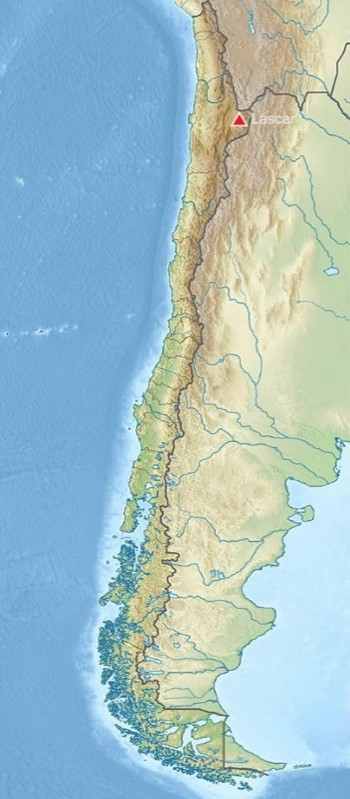
\includegraphics[width=\linewidth]{img/lascar_ubicacion.jpg}
    \caption{} \label{fig:lascar_location}
  \end{subfigure}%
  \hspace*{\fill}   % maximize separation between the subfigures
  \begin{subfigure}{0.71\textwidth}
    \footnotesize
    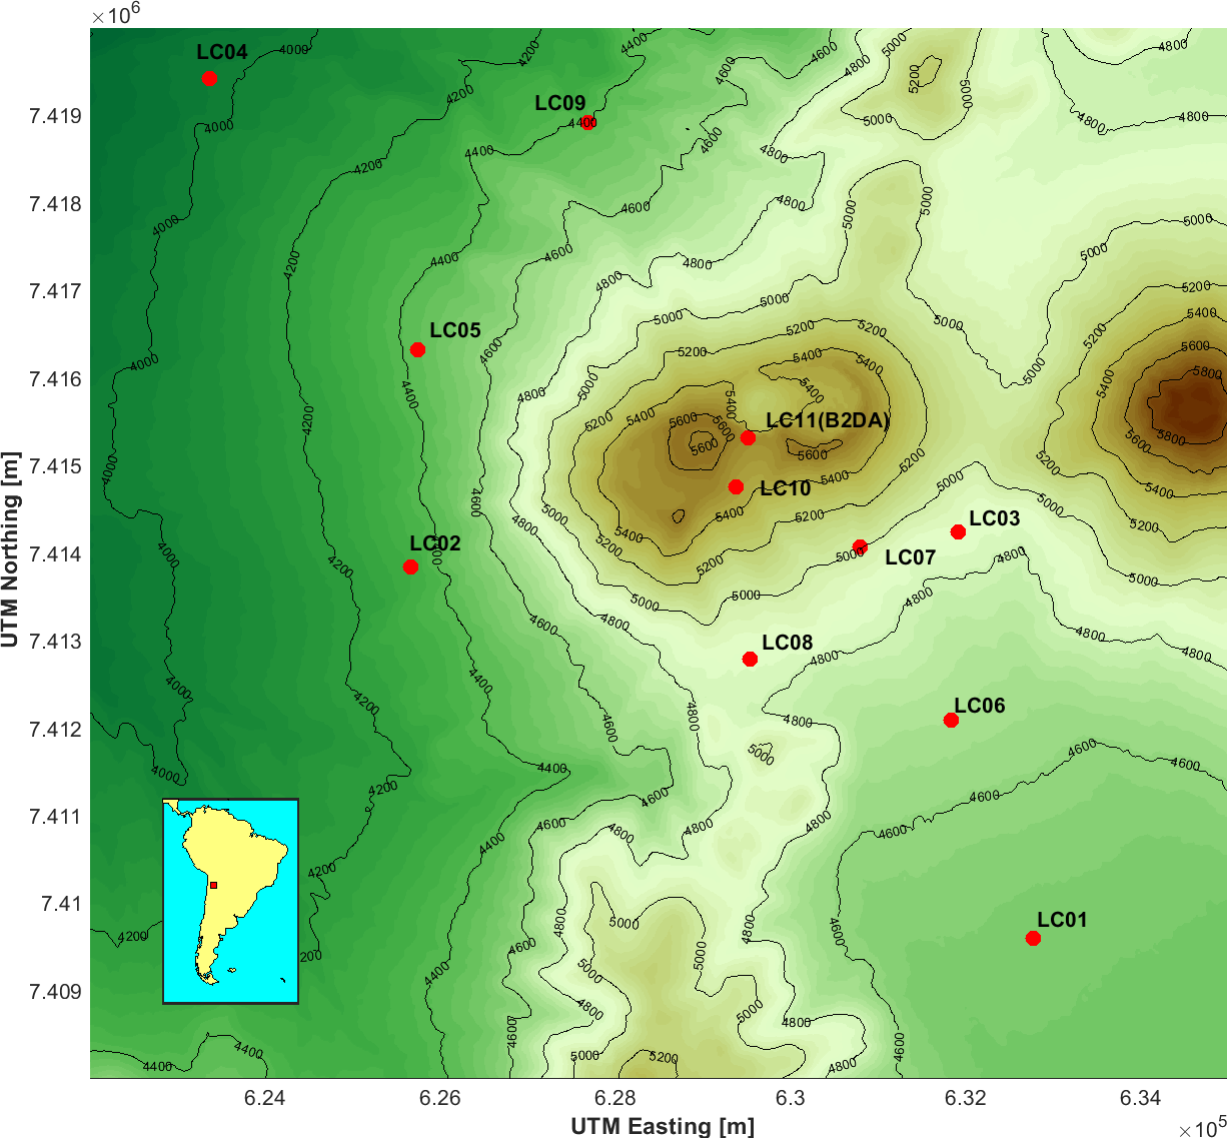
\includegraphics[width=\linewidth]{img/lascar_estaciones.png}
    \caption{} \label{fig:lascar:estations}
  \end{subfigure}%
\caption{a) Location map of Láscar volcano. b) Red dots indicate the positions of the seismic stations.}
\label{fig:lascar_map}
\end{figure*}


\subsection{Lascar's database}
The Láscar database contains 6,145 seismic events classified by geophysicist experts belonging to CKELAR-VOLCANES. The data correspond to the period between March and October 2018. The next table shows the data distribution.
\begin{table*}
\caption{Contribution of events from each station to the Lascar database.} % title of Table
\centering
\begin{adjustbox}{width=\textwidth}
\begin{tabular}{lrrrrrrrrrrrr}
\hline\hline %inserts double horizontal lines
Event\textbackslash{}Station & LC01 & LC02 & LC03 & LC04 & LC05 & LC06 & LC07 & LC08 & LC09 & LC10 & B2DA & Total \\
\hline % inserts single horizontal line
HY & 0 & 0 & 0 & 7 & 45 & 4 & 0 & 3 & 12 & 136 & 6 & 213 \\
LP & 11 & 0 & 4 & 2 & 142 & 28 & 5 & 60 & 23 & 195 & 107 & 577 \\
TC & 9 & 0 & 11 & 97 & 284 & 36 & 157 & 127 & 144 & 1,171 & 162 & 2,198 \\
TR & 1 & 0 & 5 & 29 & 21 & 4 & 61 & 13 & 35 & 292 & 10 & 471 \\
VT & 2 & 0 & 18 & 52 & 84 & 6 & 206 & 14 & 41 & 2,249 & 14 & 2,686 \\
\hline %inserts single line
TOTAL & 23 & 0 & 38 & 187 & 576 & 78 & 429 & 217 & 255 & 4,043 & 299 & 6,145 \\
\hline %inserts single line
\end{tabular}
\end{adjustbox}
\label{table:lascar_database}
\end{table*}

\begin{table*}
\caption{Statistics of the events belonging to the Láscar volcano.} % title of Table
\centering
\begin{tabular}{lrrrrrrrrrrr}
\hline\hline %inserts double horizontal lines
  Events & Quantity (\%) & Quantity & Maximum (s) & Minimum (s) & Mean (s) & Median (s) & Mode (s) & Standard Deviation (s)  \\
\hline % inserts single horizontal line
HY & 3\% & 213 & 265 & 10 & 57.2 & 59 & 40 & 35.3 \\
LP & 9\% & 577 & 600 & 9 & 82.3 & 67 & 25 & 63.5 \\
TC & 36\% & 2,198 & 670 & 9 & 78.5 & 65 & 20 & 56.2 \\
TR & 8\% & 471 & 216 & 9 & 46.2 & 31 & 20 & 33.8 \\
VT & 44\% & 2,686 & 189 & 5 & 19.6 & 17 & 10 & 12.3 \\
\hline %inserts single line
TOTAL & 100\% & 6,145 & 670 & 5 & 49.9 & 28.0 & 20 & 50.0 \\
\hline %inserts single line
\end{tabular}
\label{table:lascar_statistics}
\end{table*}


\section{Methods}\label{methods}
We proposed a solution based on transfer learning because this helps to speed up training and improve the performance of deep learning models \cite{titos2019classification,bueno2019volcano}, in addition to having few examples to generate the model again. For TL, the pre-trained AlexNet\cite{krizhevsky2012imagenet} model was considered.
The input data were spectrograms of the data labeled (waveforms) for each seismic event class. The processing sequence consists of five steps.
\begin{enumerate}
 \item describe the pre-process that applies to the time series (earthquake);
 \item detail the generation of spectrograms from the earthquakes labeled;
 \item use the data augmentation technique to increase the amount of data in training and test data sets;
 \item the construction of the prediction model; and, finally,
 \item estimate the performance of the model.
\end{enumerate}
In the following paragraphs, each step is explained.
\begin{enumerate}
  \item Pre-processing: The seismometers register data at 200Hz, 500Hz or 100Hz. We resampled at 100 Hz each event. The data were centered at the mean. A Butterworth Highpass filter was applied at 1 Hz. Then, we applied a Butterworth Bandpass filter at frequencies between 1 Hz and 10 Hz. The next step was to normalize the data. This pre-processing task was performed using the ObsPy Python toolbox \cite{beyreuther2010obspy}.
  \item The spectrograms were calculated applying a short-time Fourier transform with formula
  \begin{equation}
    S[x(t)](n,k)=\left|\sum_{m=0}^{N-1}x(m)\cdot w(m-n)\cdot e^{i2\pi mk}\right|^2
  \end{equation}
where x(t) and y(t) represent the seismic signal and short-time Fourier transform sliding window, respectively. The sliding window size was set to 1 with a 95\% overlap. The generated spectrograms are RGB images of $224\times224$ pixels.
  \item Data augmentation techniques are considered to avoid unbalanced dataset, and for that reason to avoid biased models. Many data augmentation techniques were implemented, which are presented in the next section.
  \item The pre-trained model AlexNet\cite{krizhevsky2012imagenet} was considered for the being retrained over spectrograms, using the scheme of transfer learning.
  \item The model performance is evaluated for metrics described in the next sections. The metrics is implemented on the TorchMetrics Python toolbox\footnote{\href{https://lightning.ai/docs/torchmetrics/stable}{\color{blue}https://lightning.ai/docs/torchmetrics/stable}}.
\end{enumerate}
Codes for reproducing our method are available at.\footnote{\href{https://github.com/franznet/daseismicsignals}{\color{blue}https://github.com/franznet/daseismicsignals}}



\subsection{Data Similarity}
Kullback–Leibler divergence (KL divergence) has been used to measure similarities between synthetic and real datasets, and is defined as
\begin{equation}
D_{KL}(P||Q)=\sum_{i}P(x_i )\cdot log\left(\frac{P(x_i)}{Q(x_i)}\right)
\end{equation}
where $P$ and $Q$ are the probability distributions whose distance is calculated over the samples $x_i$  of the distribution\cite{iglesias2023data}. Kullback–Leibler divergence (KL divergence) is not a symmetric distance, so it can be symmetrized to give rise to the so-called Jensen–Shannon divergence (JS divergense), defined as
\begin{equation}
JS(P||Q)=D_{KL} (P||(P+Q)/2) +D_{KL}(Q||(P+Q)/2)
\end{equation}
A measurement to quantify the distance between time series distributions. It is based on the calculation of the Wasserstein distance between time-series data. This metric is defined by measuring the Wasserstein distance of the energy between frequencies. The probability distributions have a Wasserstein–Fourier distance, which is calculated as follows\cite{iglesias2023data}:
\begin{equation}
WF([x],[y])=W_2 (s_x,s_y)
\end{equation}
where $s_x$ and $s_y$ are the normalized power spectral densities of the distributions.


\subsection{Data Augmentation}
\subsubsection{Rotation}
This transformation considers the rotation of the spectrogram around the time axis within a given percentage range of the signal length and at a given axis position. The axis position can be at the beginning, middle, or end of a spectrogram.
When applying this technique, the combination of the percentage rotation value, location of the rotation axis, and spectrogram of the event to which it will be applied is obtained. When generating new instances, care was taken to ensure that these three values were not repeated, thus ensuring unique instances in the dataset.
\begin{figure*}
\centering
{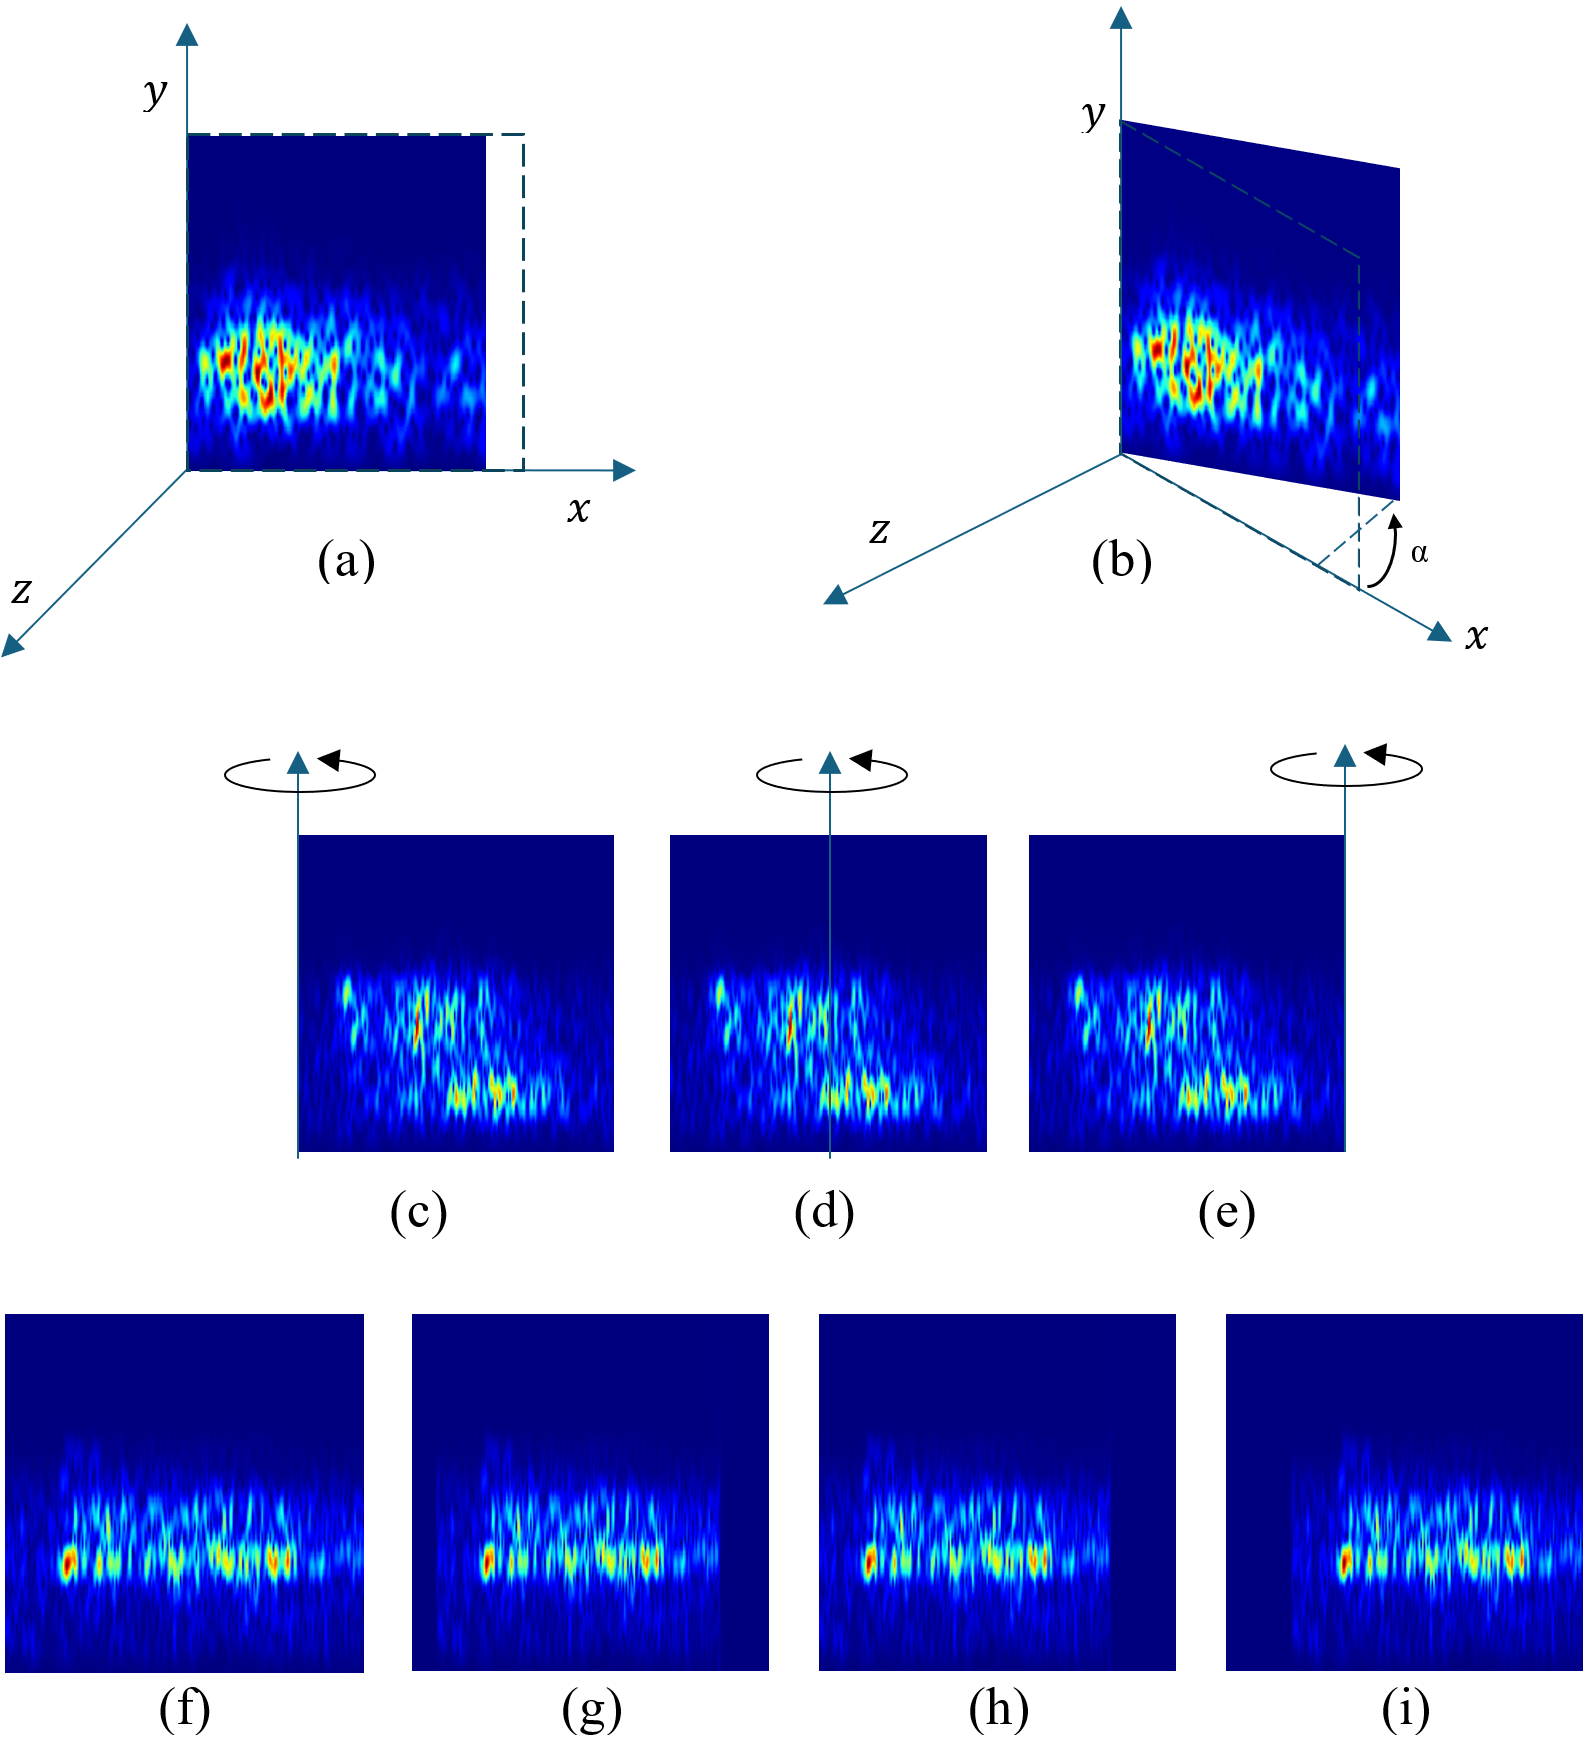
\includegraphics[width=0.6\textwidth,keepaspectratio]{img/da_rotacion.png}}
\caption{Transformation by rotations, the time stretching (a) is produced when we apply the angle of rotation (b); The possible rotation axes are located at the beginning (c), center (d), and end (e) of the spectrogram, respectively. Application examples include: (f) original spectrogram, (g) 19\% rotation around the central axis, (h) 23\% rotation around the initial axis, and (i) 24\% rotation around the final axis.}
\label{fig:da_rotation}
\end{figure*}


\subsubsection{Jittering}
Jittering is a data augmentation technique commonly employed in time series analysis\cite{iwana2021empirical,iglesias2023data}. It is considered one of the simplest yet most effective transformation-based methods, as it involves adding noise to a time series.
Formally, an original time series $x={x_1,...,x_t,...,x_T}$ is transformed into $x'={x_1+\epsilon_1,...,x_t+\epsilon_t,...,x_T+\epsilon_T}$ by introducing noise at each time step $t$, where $\epsilon$ typically represents Gaussian noise distributed as $N(\theta,\sigma^2)$. The standard deviation $\sigma$ of the added noise is a hyperparameter that must be defined in advance\cite{iwana2021empirical}.
This approach assumes that the time series patterns of a dataset are inherently noisy. Such cases may include data derived from sensors, audio signals, or electroencephalograms (EEG). For instance, jittering has been applied to wearable sensor data for Parkinson’s disease monitoring.
\begin{figure*}
\centering
{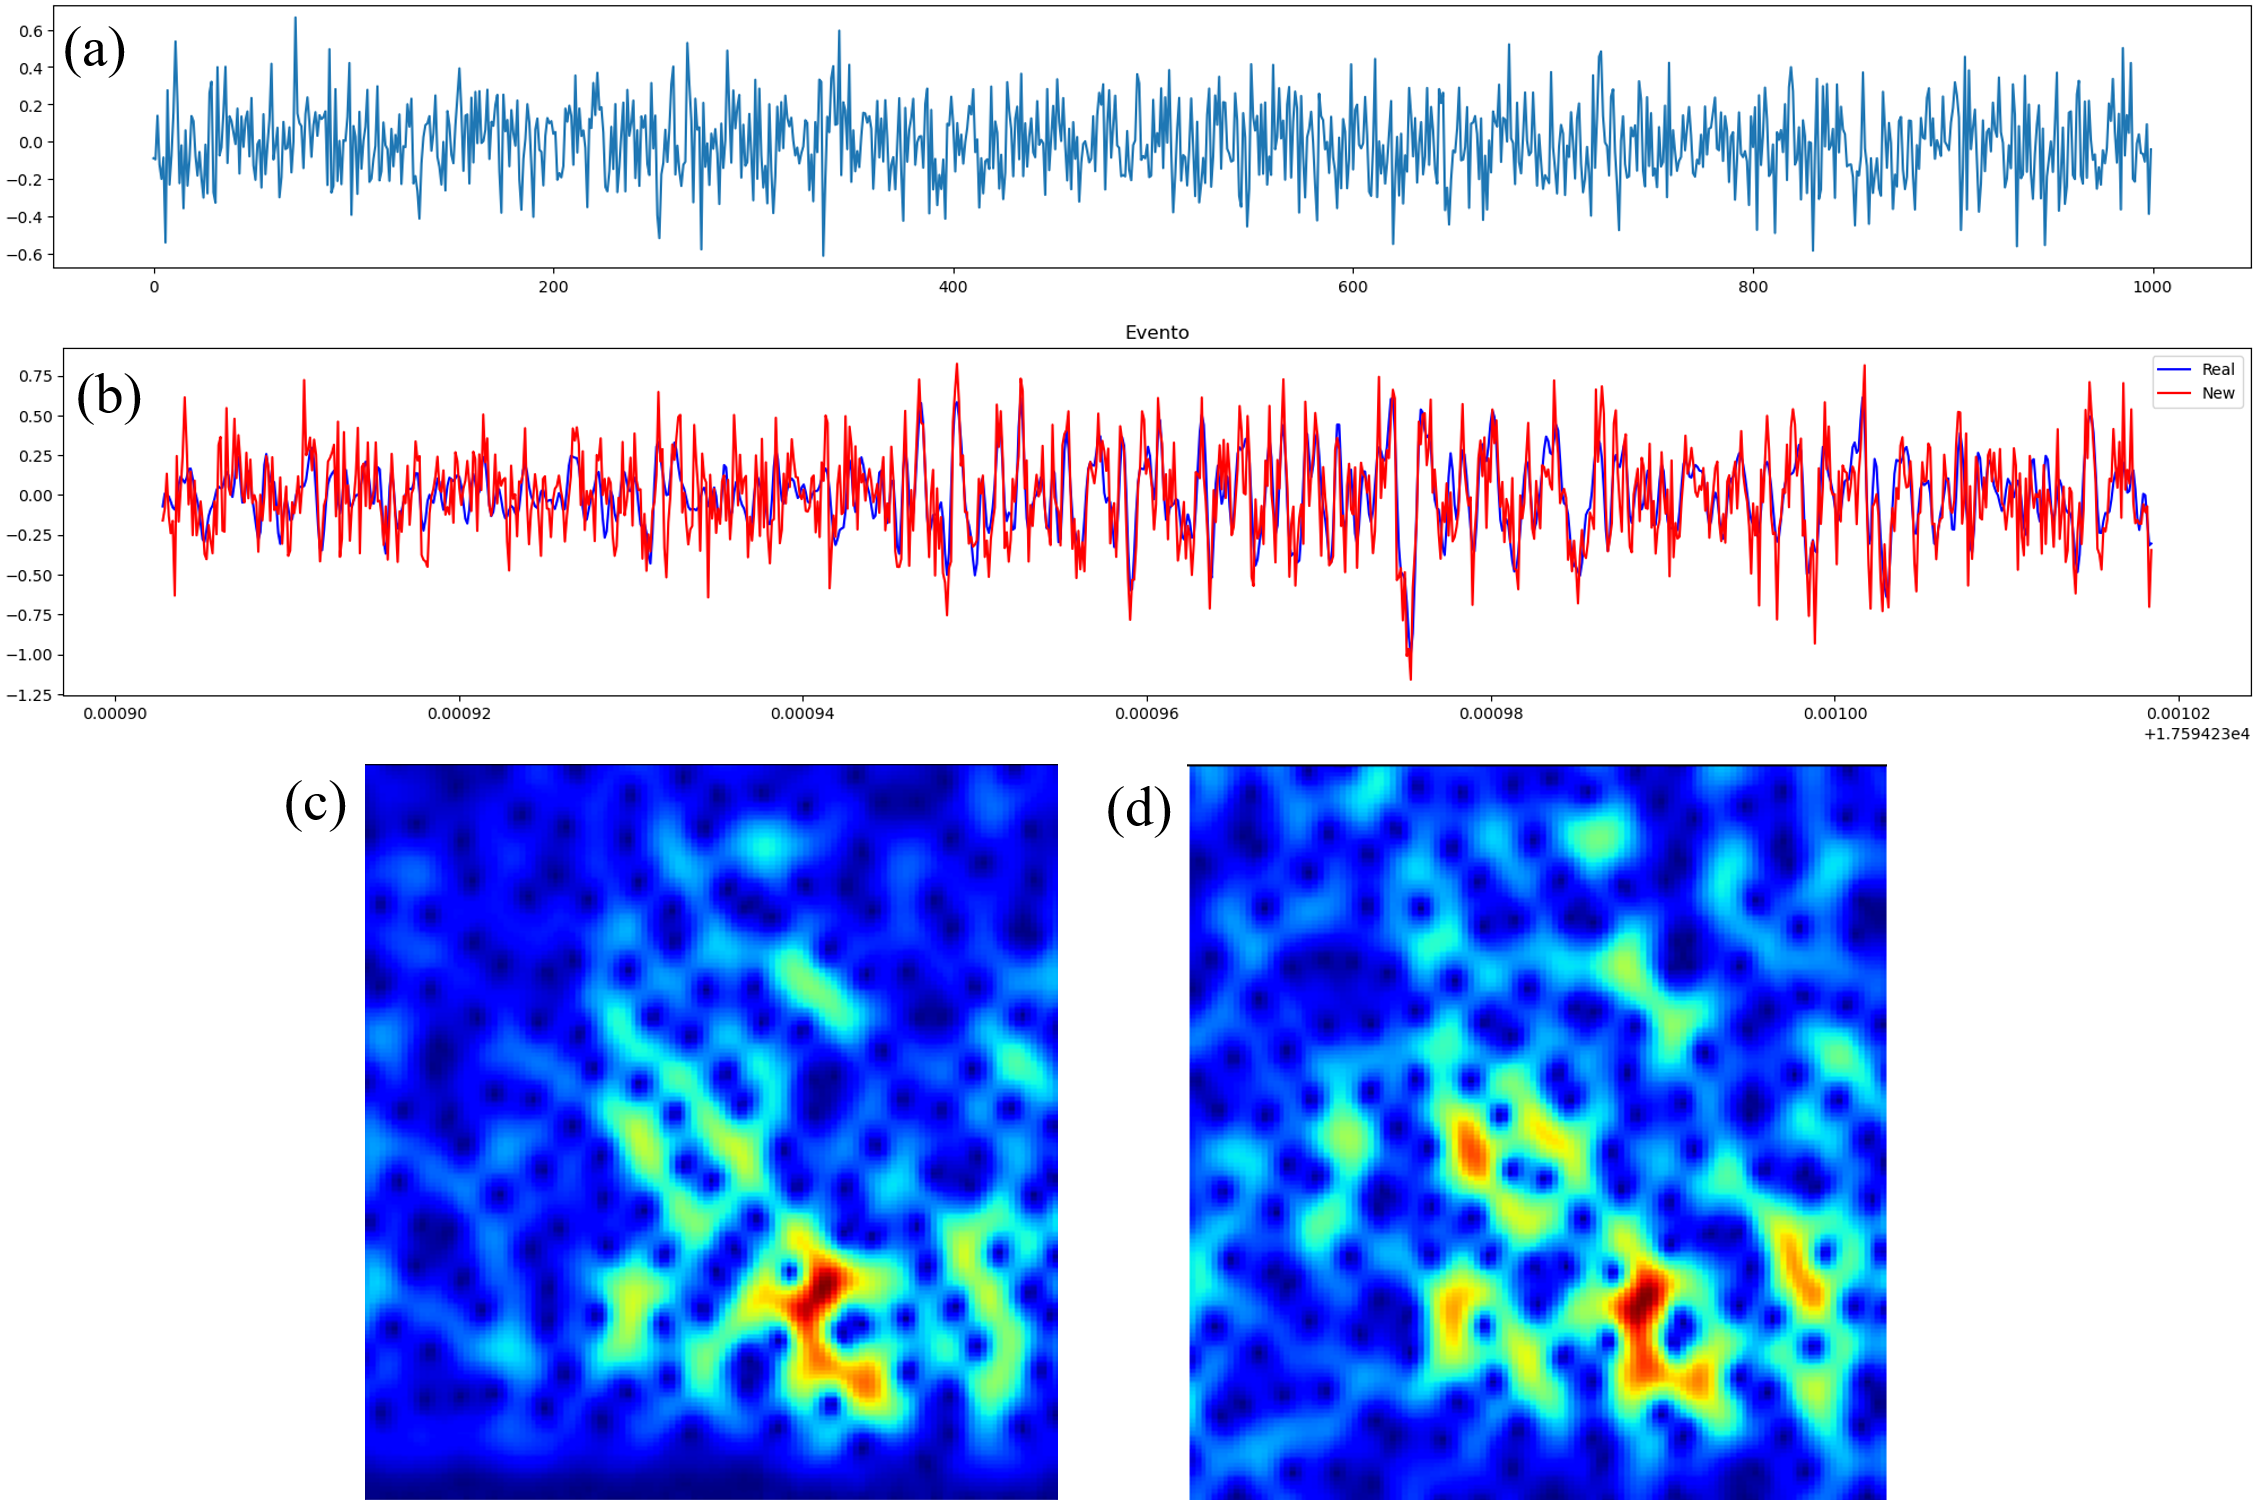
\includegraphics[width=0.8\textwidth,keepaspectratio]{img/da_jittering.png}}
\caption{Generation of a new signal using jittering. (a) Gaussian noise with distribution $N(\mu=0,\sigma=0.2)$. (b) Original (blue) and generated (red) signals. (c) Spectrogram of the original signal, and (d) spectrogram of the jittered signal.}
\label{fig:da_jittering}
\end{figure*}


\subsubsection{Drifting}
One challenge in both online and offline settings is data drift, defined as a change in the data distribution over time. A random walk is often used to simulate such drift. In mathematics, a random walk is classified as a stochastic process that represents a path composed of successive random steps in a mathematical space, such as the integers or the reals. A simple example is the integer number line $\mathrm{Z}$, where the walk begins at $\theta$ and moves either $+1$ or $-1$ with equal probability at each step. More generally, a random move of $+a$ or $-a$ with equal probability can occur in any vector space, such as the real space, where $a \in \mathrm{R}$ denotes the step magnitude\cite{fields2019mitigating}.
Let $d$ define a path starting at position $d_1=\phi(\tau)$. A random walk can then be modeled as:
\begin{equation}
d_t=d_{t-1}+\phi(\tau)
\end{equation}
where $\phi$ is the random variable describing the probability distribution for the next step, and $\tau$ is the time interval between consecutive steps. Consequently, an original time series $x={x_1,...,x_t,...,x_T}$ can be transformed into $x'={x_1+d_1,...,x_t+d_t,...,x_T+d_T}$.
Data drift simulation can be used to generate more robust training datasets, thereby enhancing model resilience and reducing sensitivity to drift when it arises in real-world data.
\begin{figure*}
\centering
{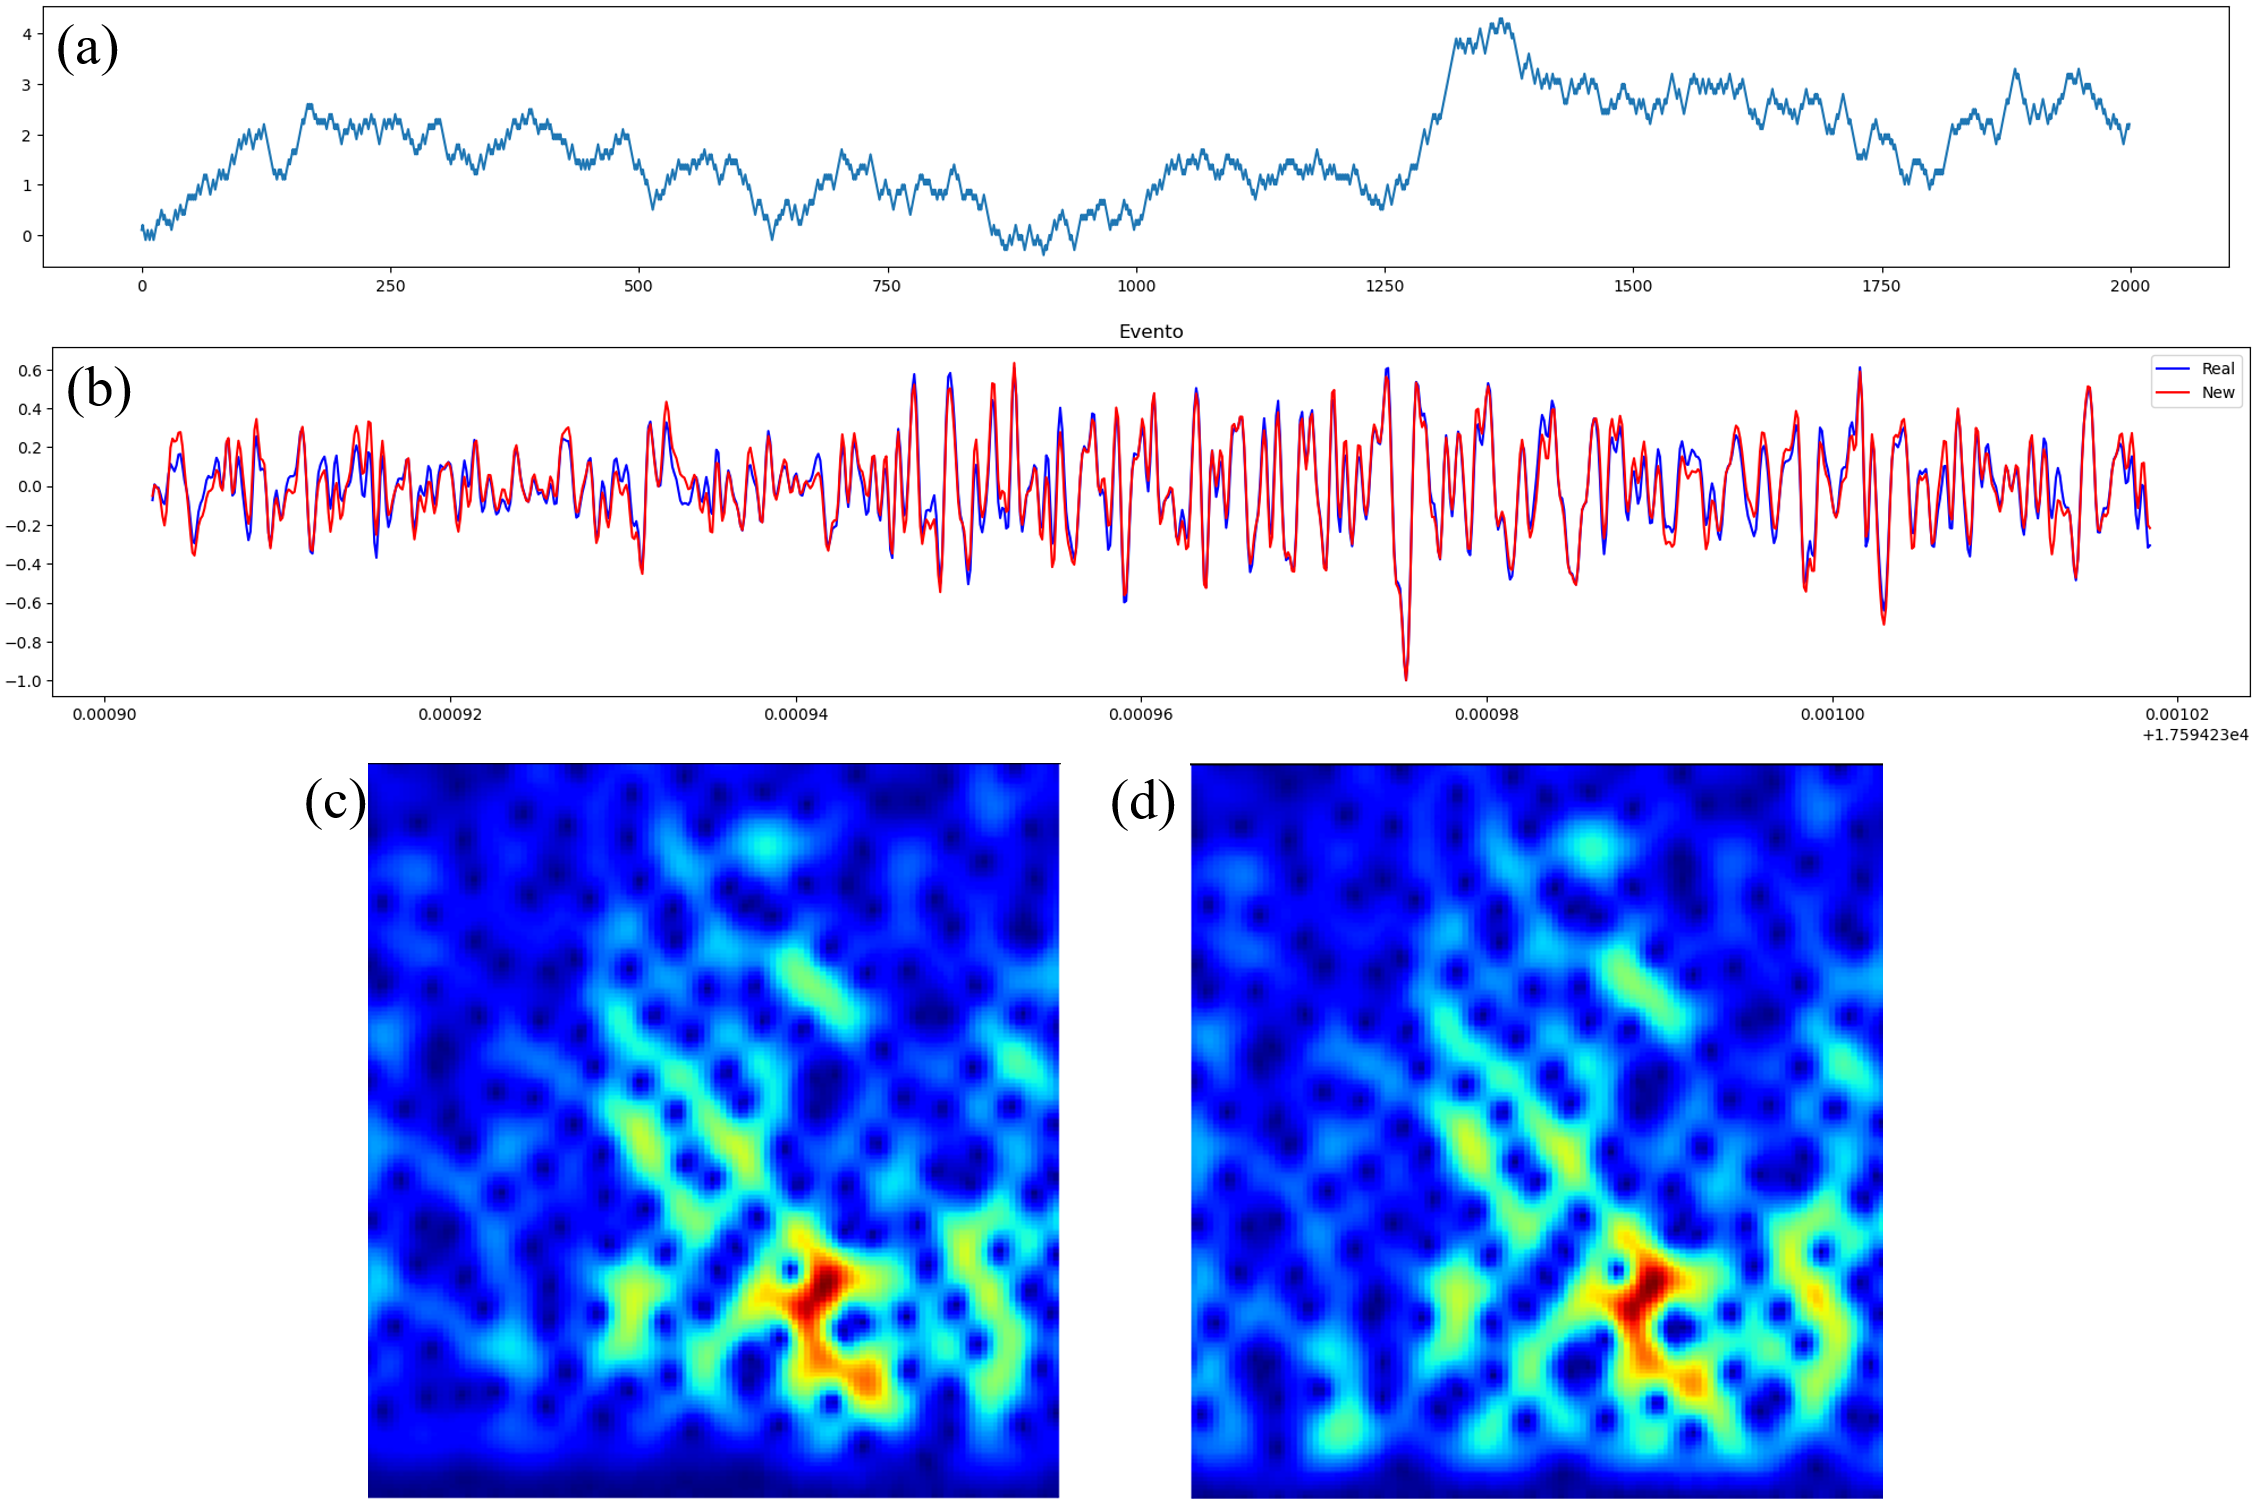
\includegraphics[width=0.8\textwidth,keepaspectratio]{img/da_drifting.png}}
\caption{Generation of a new signal using drifting. (a) Drifting signal with $\tau=0.2$. (b) Original signal (blue) and generated signal (red). (c) Spectrogram of the original signal, and (d) spectrogram of the drifted signal.}
\label{fig:da_drifting}
\end{figure*}

\subsubsection{Genetic Algorithms}
Genetic Algorithms (GA) belong to the broader class of Evolutionary Algorithms (EA) and are inspired by the principle of natural selection. Their primary objective is to generate high-quality solutions to complex problems using bio-inspired operators such as selection, crossover, and mutation\cite{nethravathi2017augmentation}. In \cite{villegas2024data}, GA have been applied to data augmentation of time series derived from centers of pressure for the detection of neuropathies.
Building on GA operators, a seismogram data augmentation technique was developed with the following procedure:
\begin{itemize}
\item \textit{Selection:} Real seismograms of the same class are selected, without repetition, to serve as parents.
\item \textit{Crossover:} Genetic information from two or more parent seismograms is combined to generate a new instance. This is achieved by exchanging time series segments between the parents’ chromosomes.
\item \textit{Mutation:} Small modifications are introduced in a limited portion of the population. In this case, a smoothing operation is applied to the scales of the exchanged segments.
\item \textit{Validation:} KL and JS divergences are used to measure similarity between datasets. Values closer to zero for both KL and JS divergences indicate greater similarity in the frequency-domain power distribution between the original and augmented seismic signals.
\end{itemize}
Two strategies were considered for the crossover operation:
\begin{itemize}
\item \textit{Without time adjustment:} The segments exchanged between parents may differ in length, resulting in a child seismogram with a duration that can vary significantly from that of the original seismograms.
\item \textit{With time adjustment:} The exchanged segments are rescaled to equal length by applying a time-scaling transformation, ensuring that the generated seismogram maintains a duration comparable to the original signals.
\end{itemize}
\begin{figure*}
\centering
{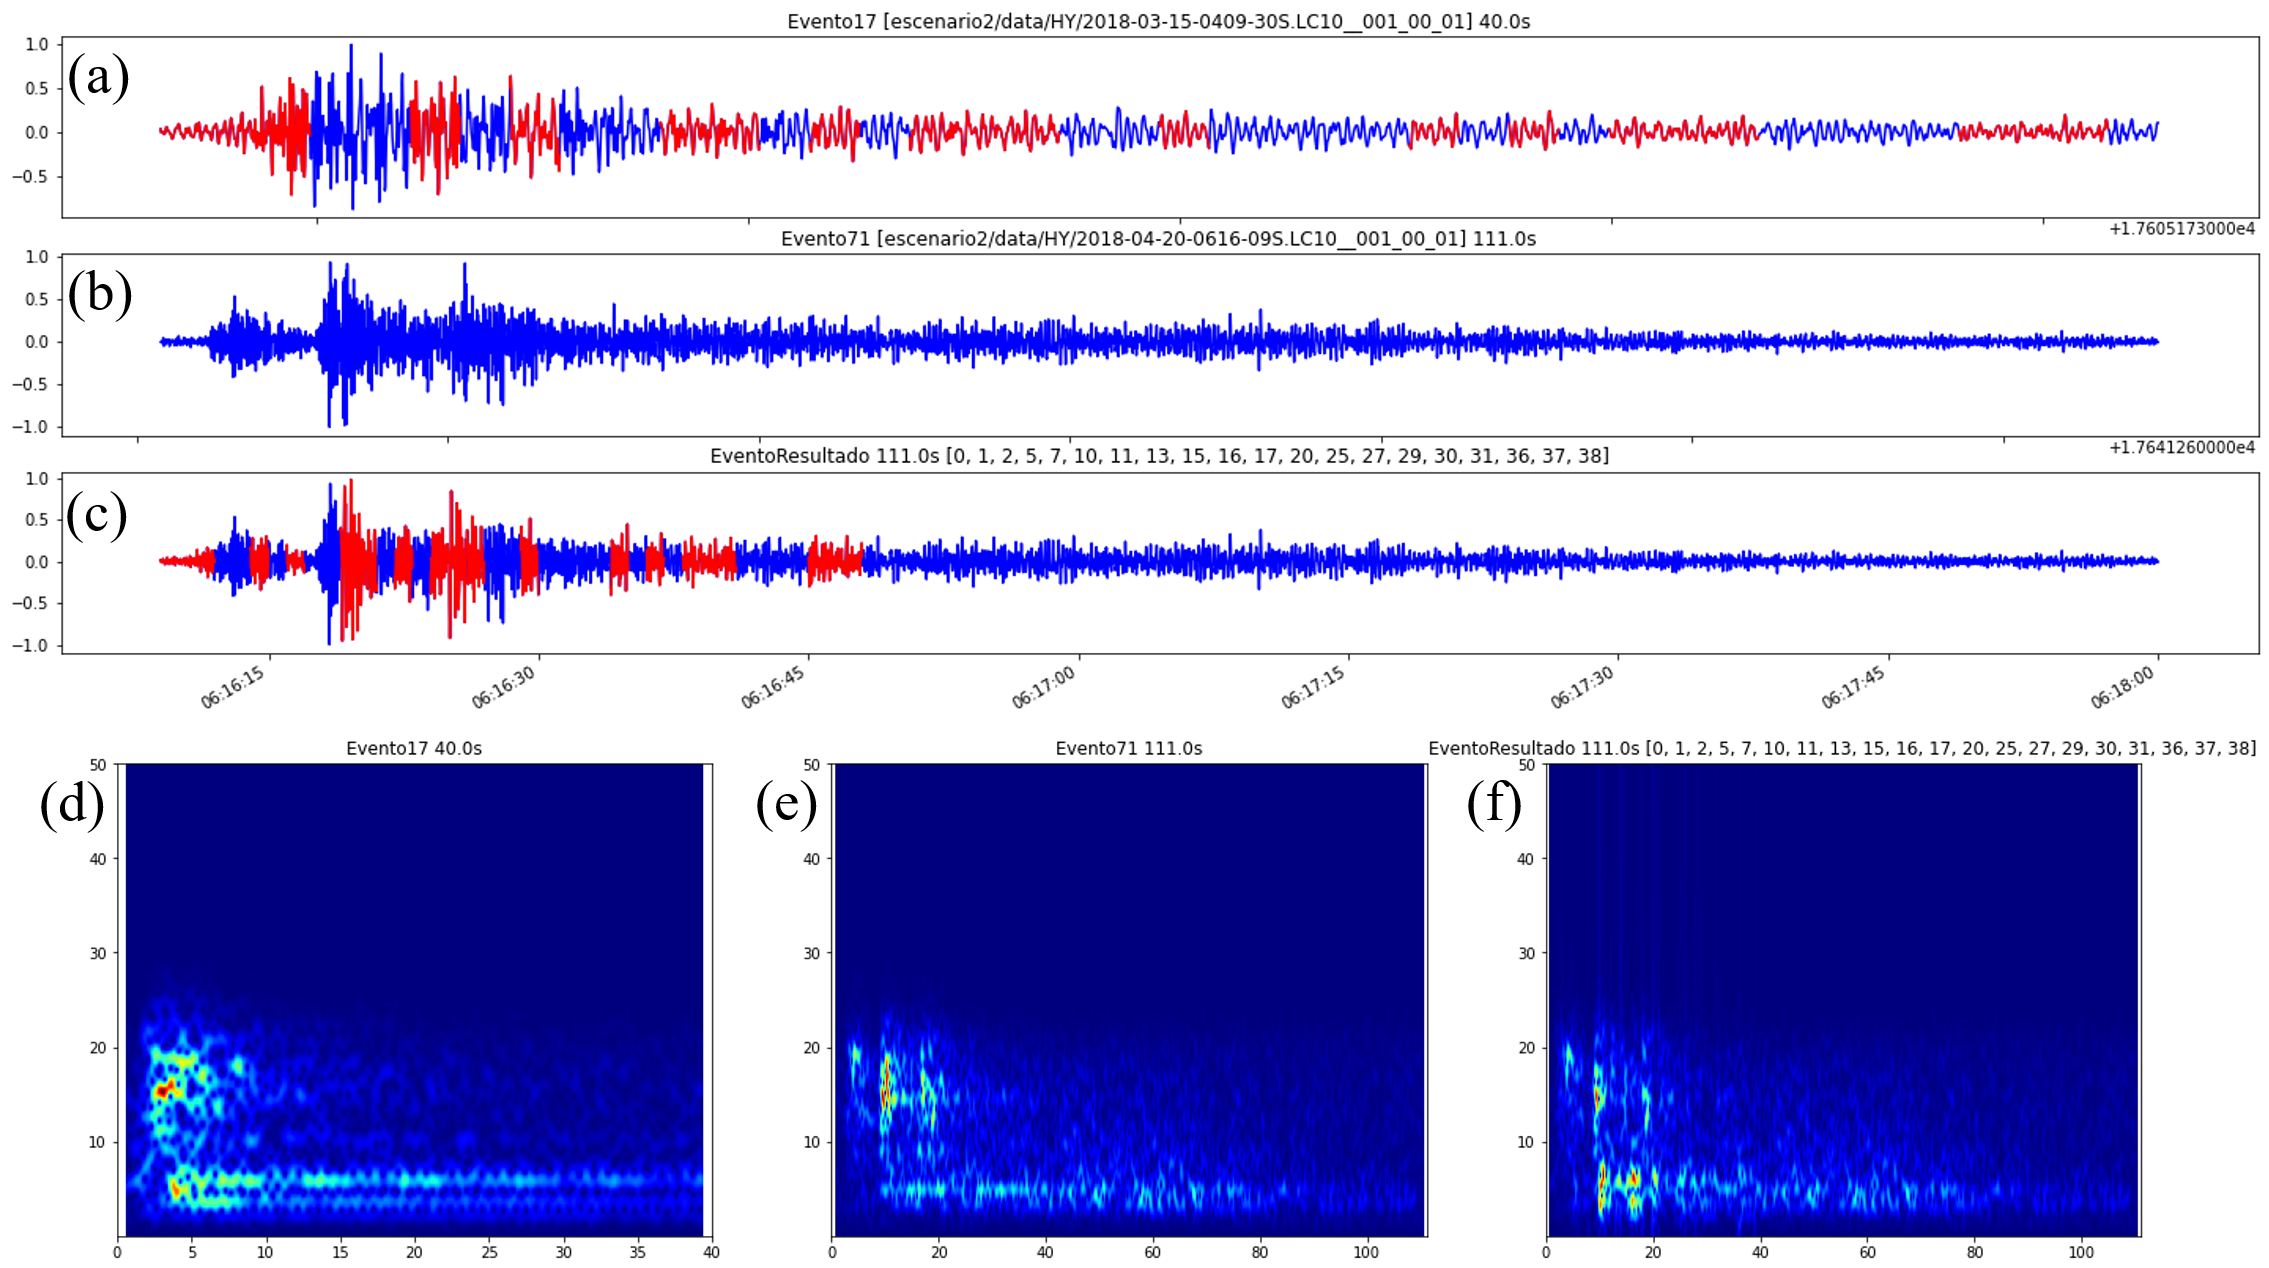
\includegraphics[width=0.8\textwidth,keepaspectratio]{img/da_ag1.png}}
\caption{Generation of a new signal using a Genetic Algorithm without time adjustment. (a) and (b) show the parent signals; the red color highlights the exchanged segments. (c) The resulting signal generated by the Genetic Algorithm. (d) and (e) show the spectrograms of the parent signals. (f) Spectrogram of the generated signal.}
\label{fig:da_ga1}
\end{figure*}
\begin{figure*}
\centering
{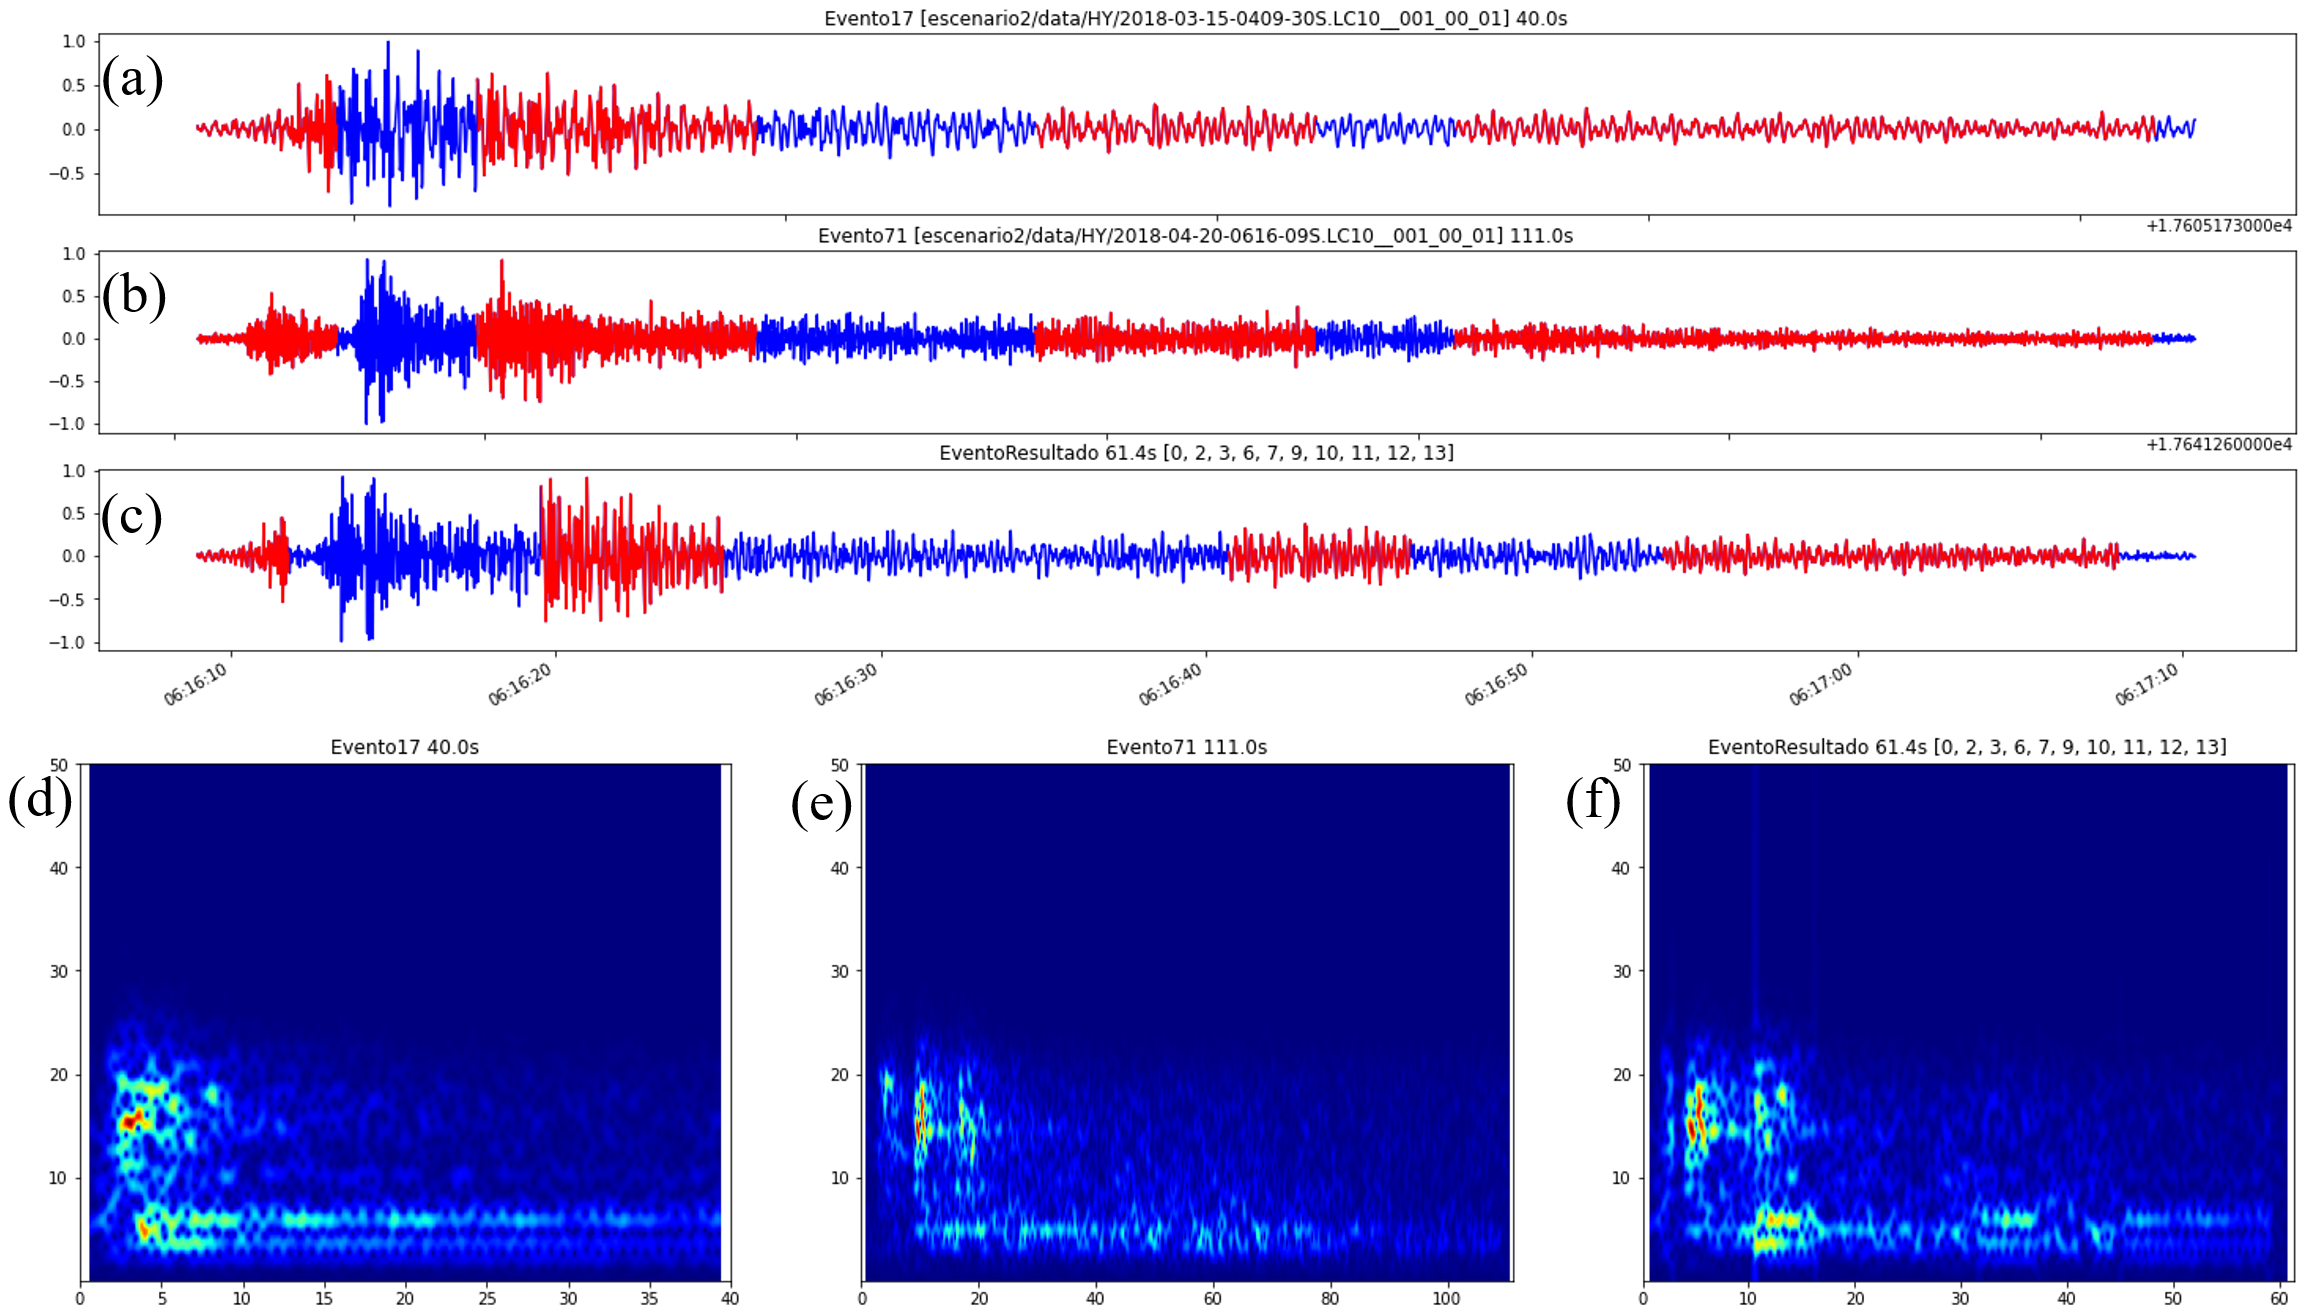
\includegraphics[width=0.8\textwidth,keepaspectratio]{img/da_ag2.png}}
\caption{Generation of a new signal using a Genetic Algorithm with time adjustment. (a) and (b) show the parent signals; the red color highlights the exchanged segments. (c) The resulting signal generated by the Genetic Algorithm. (d) and (e) display the spectrograms of the parent signals. (f) Spectrogram of the generated signal.}
\label{fig:da_ga2}
\end{figure*}

\subsubsection{SpecAugment}
SpecAugment is a data augmentation technique designed for Automatic Speech Recognition (ASR). Its primary purpose is to help the network learn useful features that are robust to time warping, to the partial loss of frequency information, and to the partial loss of small signal segments. It is a simple and computationally inexpensive method, as it acts directly on the log-mel spectrogram as if it were an image, allowing for online application during training\cite{park2019specaugment}.
SpecAugment policies consist of three main components: frequency masking, time masking, and time warping\cite{park2020specaugment,soni2024generalized}.
In this work, we apply SpecAugment on the spectrograms using frequency masking, time masking, and time warping policies.
\begin{figure*}
\centering
{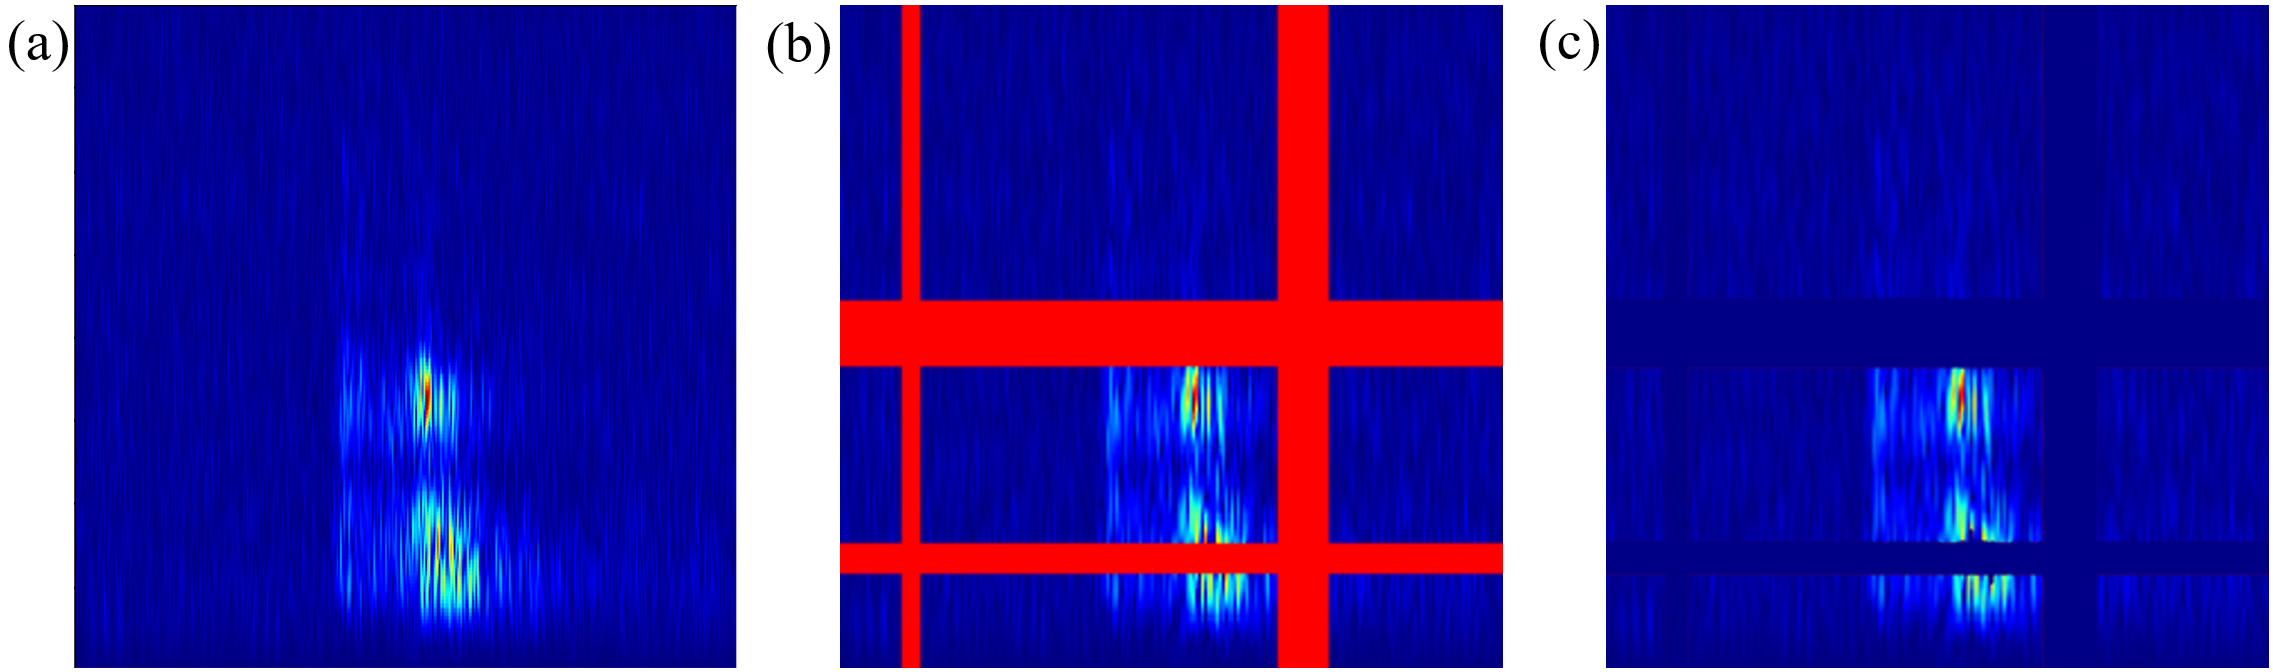
\includegraphics[width=0.8\textwidth,keepaspectratio]{img/da_specaugment.png}}
\caption{Generating new signal with SpecAugment. (a) Original spectrogram. Spectrogram with two time-frequency distortions. The distortions are shown in red (b), and with white noise in (c).
Generation of a new signal using SpecAugment. (a) The original spectrogram. (b) Spectrogram displaying two time-frequency distortions (highlighted in red). (c) Spectrogram displaying the same distortions with white noise.}
\label{fig:da_specaugment}
\end{figure*}


\subsubsection{Interpolation AEs}
Autoencoders can interpolate in certain situations by decoding the convex combination of the latent codes of two data points, thereby producing an output that semantically blends the features of the data points\cite{berthelot2018understanding}.
First, an input $x \in \mathrm{R}^{d_x}$ is passed through an encoder $z=f_\theta(x)$, parameterized by $\theta$, to obtain a latent code $z \in \mathrm{R}^{d_z}$. The latent code is then passed through a decoder $\hat{x}=g_\phi(z)$, parameterized by $\phi$, to produce an approximate reconstruction $\hat{x} \in \mathrm{R}^{d_x}$ of the input $x$. We consider the case in which both $f_\theta$ and $g_\phi$ are implemented as multi-layer neural networks. The encoder and decoder are trained jointly with respect to $\theta$ and $\phi$ to minimize a distance measure between the input $x$ and the output $\hat{x}$, such as the squared $L_2$ distance $\left|x-\hat{x}\right|^2$.
Interpolation with an autoencoder refers to the process of using the decoder $g_\phi$ to reconstruct a mixture of two latent codes. Typically, the latent codes are combined via a convex combination, so that interpolation amounts to computing $x_\alpha=g_\phi(\alpha z_1+(1-\alpha) z_2)$ for some $\alpha \in [0,1]$, where $z_1=f_\theta(x_1)$ and $z_2=f_\theta(x_2)$ are the latent codes corresponding to the data points $x_1$ and $x_2$.
\begin{figure*}
\centering
{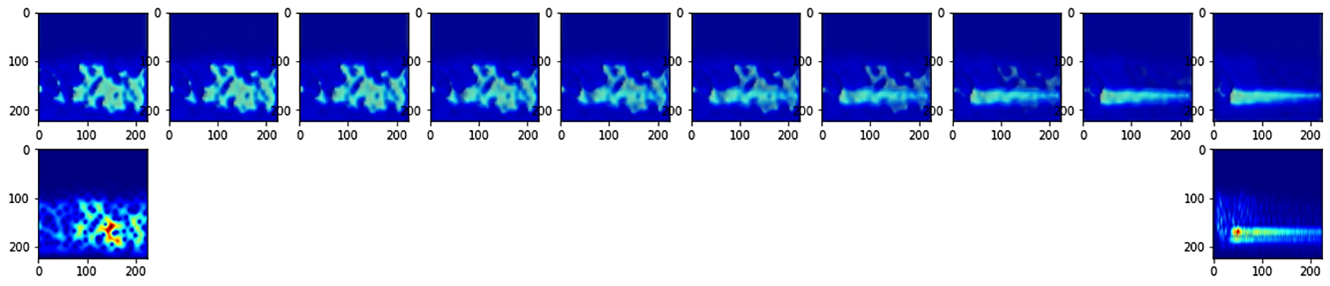
\includegraphics[width=0.9\textwidth,keepaspectratio]{img/da_interpolacion.png}}
\caption{Interpolating events (HY) at different intensity levels yields greater diversity.}
\label{fig:da_interpolation}
\end{figure*}


\subsection{Model performance - Metrics}
Machine learning metrics make it possible to quantify the performance of a trained model and to compare it with other generated models or with the current baseline. Evaluating the learning algorithm is a crucial part of any project. While classification accuracy is most commonly used to assess model performance, it is insufficient on its own to provide a complete evaluation. Therefore, various complementary evaluation metrics are considered.
Among the different classification metrics, we can mention:
\begin{itemize}
\item \textit{Confusion Matrix:} A tabular representation of true labels versus model predictions. Although not a performance metric in itself, it serves as the foundation for deriving many other evaluation measures.
\begin{table}
\caption{Confusion matrix.}
\centering
\begin{tblr}{
  cell{1}{3} = {c=2}{c},
  cell{2}{3} = {c},
  cell{2}{4} = {c},
  cell{3}{1} = {r=2}{},
  hline{2} = {3-4}{},
  hline{3,5} = {-}{},
}
% \hline
 &  & Predicted & \\
 &  & Positive (P) & Negative (N)\\
Actual & Positive (P) & True positive (TP) & False negative (FN)\\
 & Negative (N) & False positive (FP) & True negative (TN)\\
\end{tblr}
\label{table:confusion_matrix}
\end{table}

Where $TP$ denotes true positives, $TN$ true negatives, $FP$ false positives, and $FN$ false negatives.
\item \textit{Recall (Sensitivity):} Measures the proportion of actual positive cases that the model correctly identifies.
\begin{equation}
Recall=\frac{TP}{TP+FN}
\end{equation}
\item \textit{Precision:} Measures the proportion of positive predictions that are correct, indicating the model’s reliability in classification tasks.
\begin{equation}
Precision=\frac{TP}{TP+FP}
\end{equation}
\item $F_\beta$: Combines precision and recall into a single value, facilitating comparison across models. The parameter $\beta > 0$ adjusts the relative importance of recall versus precision: values $\beta>1$ favor recall, while $\beta<1$ favor precision. This metric is particularly useful for imbalanced datasets.
\begin{equation}
F_\beta=(1+\beta^2)\cdot \frac{precision\cdot recall}{\beta^2 \cdot precision+recall}
\end{equation}
\item \textit{Acurracy:} Measures the overall proportion of correctly classified cases. However, it can be misleading when dealing with imbalanced datasets.
\begin{equation}
Accuracy=\frac{TP+TN}{TP+TN+FP+FN}
\end{equation}
\item \textit{Specificity:} Measures the proportion of actual negative cases that the model correctly identifies.
\begin{equation}
Specificity=\frac{TN}{TN+FP}
\end{equation}
\end{itemize}


\subsection{Evaluation metrics for data augmentation}
Data augmentation techniques have become a widely adopted strategy for improving the generalization capacity of deep neural networks. An important consideration in this context is the balance between similarity and diversity in the data \cite{yang2024investigating}. Similarity reflects the degree of resemblance between the original and augmented data, whereas diversity captures the variation in complexity introduced through augmentation. 
These metrics were calculated using the framework Python TorchMetrics\footnote{\href{https://lightning.ai/docs/torchmetrics/stable}{\color{blue}https://lightning.ai/docs/torchmetrics/stable}} de Lightning AI, the creators of PyTorch Lightning.


\subsubsection{Fréchet Inception Distance (FID)}
The Fréchet Inception Distance (FID) is a widely used metric for evaluating the quality of images generated by Generative Adversarial Networks (GANs)\cite{guven2024image}. Its primary objective is to quantify the similarity between generated and real images\cite{heusel2017gans}. Compared to earlier metrics such as the Inception Score (IS), the FID offers an improvement because it leverages statistics from real-world samples for comparison, whereas the IS does not\cite{kynkäänniemi2023roleimagenetclassesfrechet}.
The core idea of the FID is to embed both real and generated images into a vision-relevant feature space and then compute the distance between the distributions of these embeddings. In practice, this feature space is typically the penultimate layer (pool3, with 2048 features) of an Inception-V3 classifier pre-trained on ImageNet\cite{kynkäänniemi2023roleimagenetclassesfrechet}.
\begin{equation}
FID(\mu_r,\Sigma_r,\mu_g,\Sigma_g )=\left\|\mu_r-\mu_g \right\|_2^2+Tr(\Sigma_r+\Sigma_g-2(\Sigma_r \Sigma_g)^{\frac{1}{2}})
\end{equation}
where $(\mu_r,\Sigma_r)$ and $(\mu_g,\Sigma_g)$ denote the sample main and covariance of the embeddings of the real and generated data, respectively, and $Tr(\cdot)$ indicates the matrix trace\cite{kynkäänniemi2023roleimagenetclassesfrechet}.
The theoretical range of the FID is $[0, \infty)$, as it is a distance measure. Lower values correspond to higher-quality images\cite{wang2019improvingmmdgantrainingrepulsive}. In theory, an FID of 0 indicates that the feature distributions of the generated and real images are identical in terms of mean and covariance under the Gaussian approximation\cite{heusel2017gans}.
Empirical studies have shown that FID correlates well with human judgments of image fidelity\cite{heusel2017gans}. 


\subsubsection{Kernel Inception Distance (KID)}
The squared Maximum Mean Discrepancy (MMD) is used by the Kernel Inception Distance (KID) to measure the difference between the feature representations of real and generated images. These features are extracted from the Inception network. Unlike the Fréchet Inception Distance (FID)\cite{heusel2017gans}, KID employs an unbiased estimator, which makes it more reliable, particularly when the number of test images is smaller than the dimensionality of the Inception features. A lower KID score indicates greater visual similarity between real and generated images\cite{kim2019ugatit}.
KID use a polynomial kernel $k(x,y)=(\frac{1}{d}x^T\cdot y+1)^3$ where $d$ is the dimension of the Inception representation vector, and $x$ and $y$ are two feature vectors. The kernel $K(x,y)=k(\phi(x),\phi(y))$ can then be applied as an MMD for input images, where images are mapped into Inception representations through $\phi$\cite{binkowski2018demystifying}.
Since KID is a distance metric, a value of 0 indicates a perfect match between the distributions of real and generated features. Theoretically, if the two distributions are identical, the distance equals zero. A key advantage of KID lies in its simple and unbiased estimator, which distinguishes it from FID\cite{binkowski2018demystifying}.

\subsubsection{Multi-Scale Structural Similarity (MS-SSIM)}
MS-SSIM is a multi-scale improvement of SSIM that aims to eliminate aspects of an image that are not crucial for human perception \cite{wang2003multiscale,ma2016group}. The calculation of SSIM, which serves as the basis for MS-SSIM, compares three principal components: luminance (intensity), contrast, and structure. It employs basic statistical moments, such as the mean and standard deviation, within local windows to derive a similarity score.
\begin{equation}
MS-SSIM(x,y)=\left[l_M (x,y)\right]^{\alpha_M}\cdot \prod_{j=1}^{M}\left[c_j(x,y)\right]^{\beta_j}\cdot \left[s_j (x,y)\right]^{\gamma_j}
\end{equation}
where $l_M (x,y)$ represents the luminance component between images $x$ and $y$, $c_j(x,y)$ denotes the contrast component at scale $j$, and $s_j(x,y)$ reflects the structural similarity in scale $j$. The parameters $\alpha_M$, $\beta_j$, and $\gamma_j$ define the relative importance of the luminance, contrast, and structure components, respectively. Lastly, $M$ signifies the number of scales employed in the MS-SSIM calculation\cite{arsenio2025recovering}.
The range of MS-SSIM values is between 0 and 1, and images with higher MS-SSIM values are perceived as more similar\cite{odena2017conditional}, with 1 indicating perfect similarity. Lower MS-SSIM scores indicate higher diversity\cite{guo2019autoembedding,wang2019improvingmmdgantrainingrepulsive}.
Unlike metrics such as FID (Fréchet Inception Distance) or KID (Kernel Inception Distance), MS-SSIM does not require a pre-trained Inception network\cite{fahim2020alightweight}. Therefore, the use of IS, KID, or FID is not recommended, as these metrics inherently utilize weights from the Inception network, which are validated for images similar to those in the ImageNet dataset. Consequently, these metrics cannot be applied to datasets outside ImageNet. MS-SSIM  was applied to a fingerprint dataset\cite{fahim2020alightweight}.
Lower FID values indicate superior image quality, and lower MS-SSIM scores reflect increased diversity \cite{guo2019autoembedding}. Smaller FID and KID values correlate with more realistic images in image translation \cite{torbunov2023rethinking}.
Considering that our spectrogram dataset is not part of the ImageNet dataset, we utilized the MS-SSIM score.


\begin{table*}
\caption{Statistics related to the transfer learning over AlexNet pre-trained model.}
\centering
\begin{adjustbox}{width=\textwidth}
\begin{tabular}{lllcrrrrr}
\hline\hline %inserts double horizontal lines
Dataset & Data type & Data Augmentation & Balanced dataset & Epochs & Total data & Train data & Test data & Training time (min.) \\
\hline % inserts single horizontal line
(i) & Real & No & NO & 10 & 6,145 & 4,916 & 1,229 & 4.2 \\
(ii) & Real + Augmented & Rotation(5\%-25\%) & YES & 20 & 13,430 & 10,744 & 2,686 & 18.7 \\
(iii) & Augmented & Rotation(5\%-25\%) & YES & 20 & 13,430 & 10,744 & 2,686 & 20.9 \\
(iv) & Real + Augmented & Jittering(0.2) & YES & 20 & 13,430 & 10,744 & 2,686 & 16.8 \\
(v) & Augmented & Jittering(0.2) & YES & 20 & 13,430 & 10,744 & 2,686 & 17.2 \\
(vi) & Real + Augmented & Drifting Drift(0.01-0.1) & YES & 20 & 13,430 & 10,744 & 2,686 & 17.9 \\
(vii) & Augmented & Drifting
  Drift(0.01-0.1) & YES & 20 & 13,430 & 10,744 & 2,686 & 20.3 \\
(viii) & Real + Augmented & Drifting Drift(0.001-0.01) & YES & 20 & 13,430 & 10,744 & 2,686 & 21.7 \\
(ix) & Augmented & Drifting
  Drift(0.001-0.01) & YES & 20 & 13,430 & 10,744 & 2,686 & 21.0 \\
(x) & Real + Augmented & Drifting Drift(0.0001-0.001) & YES & 20 & 13,430 & 10,744 & 2,686 & 18.1 \\
(xi) & Augmented & Drifting Drift(0.0001-0.001) & YES & 20 & 13,430 & 10,744 & 2,686 & 20.9 \\
(xii) & Real + Augmented & Genetic Algorithm
  Segment Size(5s) Crossover Segments(3) & YES & 20 & 13,430 & 10,744 & 2,686 & 16.7 \\
(xiii) & Augmented & Genetic Algorithm Segment Size(5s) Crossover
  Segments(3) & YES & 20 & 13,430 & 10,744 & 2,686 & 17.0 \\
(xiv) & Real + Augmented & Genetic Algorithm
  Segment Size(5s) Crossover Segments(5) & YES & 20 & 13,430 & 10,744 & 2,686 & 16.6 \\
(xv) & Augmented & Genetic Algorithm Segment Size(5s) Crossover
  Segments(5) & YES & 20 & 13,430 & 10,744 & 2,686 & 16.9 \\
(xvi) & Real + Augmented & Genetic Algorithm
  Signal Percent(40\%) Crossover Segments(10) & YES & 20 & 13,430 & 10,744 & 2,686 & 16.6 \\
(xvii) & Augmented & Genetic Algorithm Signal Percent(40\%) Crossover
  Segments(10) & YES & 20 & 13,430 & 10,744 & 2,686 & 17.3 \\
(xviii) & Real + Augmented & Genetic Algorithm
  Signal Percent(45\%) Crossover Segments(10) & YES & 20 & 13,430 & 10,744 & 2,686 & 16.5 \\
(xix) & Augmented & Genetic Algorithm Signal Percent(45\%) Crossover
  Segments(10) & YES & 20 & 13,430 & 10,744 & 2,686 & 17.1 \\
(xx) & Real + Augmented & SpecAugment
  Frequency Percent(0\%-10\%) Frequency Masks(2) Time Percent(0\%-10\%) Time
  Marks(2) & YES & 20 & 13,430 & 10,744 & 2,686 & 16.5 \\
(xxi) & Augmented & SpecAugment Frequency Percent(0\%-10\%) Frequency
  Masks(2) Time Percent(0\%-10\%) Time Marks(2) & YES & 20 & 13,430 & 10,744 & 2,686 & 17.0 \\
(xxii) & Real + Augmented & SpecAugment
  Frequency Percent(0\%-15\%) Frequency Masks(2) Time Percent(0\%-15\%) Time Marks(2) & YES & 20 & 13,430 & 10,744 & 2,686 & 16.6 \\
(xxiii) & Augmented & SpecAugment Frequency Percent(0\%-15\%) Frequency
  Masks(2) Time Percent(0\%-15\%) Time Marks(2) & YES & 20 & 13,430 & 10,744 & 2,686 & 16.9 \\
(xxiv) & Real + Augmented & Interpolation AE Signal percent(40\%-60\%) & YES & 20 & 13,430 & 10,744 & 2,686 & 16.6 \\
(xxv) & Augmented & Interpolation
  AE Signal percent(40\%-60\%) & YES & 20 & 13,430 & 10,744 & 2,686 & 17.9 \\
\hline %inserts single line
\end{tabular}
\end{adjustbox}
\label{table:training_statistic}
\end{table*}


\begin{table*}
\caption{Performance of transfer learning models trained to 1-20 [Hz].}
\centering
\begin{adjustbox}{width=\textwidth}
\begin{tblr}{
  row{2} = {c},  column{3} = {c},  column{4} = {c},  column{5} = {c},
  column{6} = {c},  column{7} = {c},  cell{1}{1} = {r=2}{},  cell{1}{2} = {r=2}{},
  cell{1}{3} = {r=2}{},  cell{1}{4} = {r=2}{},  cell{1}{5} = {r=2}{},  cell{1}{6} = {r=2}{},
  cell{1}{7} = {r=2}{},  cell{1}{8} = {c=5}{c},  cell{3}{8} = {c},  cell{3}{9} = {c},
  cell{3}{10} = {c},  cell{3}{11} = {c},  cell{3}{12} = {c},  cell{4}{8} = {c},
  cell{4}{9} = {c},  cell{4}{10} = {c},  cell{4}{11} = {c},  cell{4}{12} = {c},
  cell{5}{8} = {c},  cell{5}{9} = {c},  cell{5}{10} = {c},  cell{5}{11} = {c},
  cell{5}{12} = {c},  cell{6}{8} = {c},  cell{6}{9} = {c},  cell{6}{10} = {c},
  cell{6}{11} = {c},  cell{6}{12} = {c},  cell{7}{8} = {c},  cell{7}{9} = {c},
  cell{7}{10} = {c},  cell{7}{11} = {c},  cell{7}{12} = {c},  cell{8}{8} = {c},
  cell{8}{9} = {c},  cell{8}{10} = {c},  cell{8}{11} = {c},  cell{8}{12} = {c},
  cell{9}{8} = {c},  cell{9}{9} = {c},  cell{9}{10} = {c},  cell{9}{11} = {c},
  cell{9}{12} = {c},  cell{10}{8} = {c},  cell{10}{9} = {c},  cell{10}{10} = {c},
  cell{10}{11} = {c},  cell{10}{12} = {c},  cell{11}{8} = {c},  cell{11}{9} = {c},
  cell{11}{10} = {c},  cell{11}{11} = {c},  cell{11}{12} = {c},  cell{12}{8} = {c},
  cell{12}{9} = {c},  cell{12}{10} = {c},  cell{12}{11} = {c},  cell{12}{12} = {c},
  cell{13}{8} = {c},  cell{13}{9} = {c},  cell{13}{10} = {c},  cell{13}{11} = {c},
  cell{13}{12} = {c},  cell{14}{8} = {c},  cell{14}{9} = {c},  cell{14}{10} = {c},
  cell{14}{11} = {c},  cell{14}{12} = {c},  cell{15}{8} = {c},  cell{15}{9} = {c},
  cell{15}{10} = {c},  cell{15}{11} = {c},  cell{15}{12} = {c},  cell{16}{8} = {c},
  cell{16}{9} = {c},  cell{16}{10} = {c},  cell{16}{11} = {c},  cell{16}{12} = {c},
  cell{17}{8} = {c},  cell{17}{9} = {c},  cell{17}{10} = {c},  cell{17}{11} = {c},
  cell{17}{12} = {c},  cell{18}{8} = {c},  cell{18}{9} = {c},  cell{18}{10} = {c},
  cell{18}{11} = {c},  cell{18}{12} = {c},  cell{19}{8} = {c},  cell{19}{9} = {c},
  cell{19}{10} = {c},  cell{19}{11} = {c},  cell{19}{12} = {c},  cell{20}{8} = {c},
  cell{20}{9} = {c},  cell{20}{10} = {c},  cell{20}{11} = {c},  cell{20}{12} = {c},
  cell{21}{8} = {c},  cell{21}{9} = {c},  cell{21}{10} = {c},  cell{21}{11} = {c},
  cell{21}{12} = {c},  cell{22}{8} = {c},  cell{22}{9} = {c},  cell{22}{10} = {c},
  cell{22}{11} = {c},  cell{22}{12} = {c},  cell{23}{8} = {c},  cell{23}{9} = {c},
  cell{23}{10} = {c},  cell{23}{11} = {c},  cell{23}{12} = {c},  cell{24}{8} = {c},
  cell{24}{9} = {c},  cell{24}{10} = {c},  cell{24}{11} = {c},  cell{24}{12} = {c},
  cell{25}{8} = {c},  cell{25}{9} = {c},  cell{25}{10} = {c},  cell{25}{11} = {c},
  cell{25}{12} = {c},  cell{26}{8} = {c},  cell{26}{9} = {c},  cell{26}{10} = {c},
  cell{26}{11} = {c},  cell{26}{12} = {c},  cell{27}{8} = {c},  cell{27}{9} = {c},
  cell{27}{10} = {c},  cell{27}{11} = {c},  cell{27}{12} = {c},  hline{2} = {8-12}{},
  hline{3} = {-}{},
}
\hline\hline %inserts double horizontal lines
Dataset & Data
  augmentation & Accuracy & F1 & Recall & Precision & Cohen Kappa & Class
  Accuracy &  &  &  & \\
 &  &  &  &  &  &  & HY & LP & TC & TR & VT\\
(i) & No & 62.8 & 63.9 & 62.8 & 66.7 & 67.6 & 38.9 & 74.8 & 73.5 & 33.3 & 93.4\\
(ii) & Rotation(5\%-25\%) & 91.5 & 91.4 & 91.5 & 91.4 & 89.2 & 98.4 & 92.4 & 83.5 & 93.3 & 89.6\\
(iii) & Rotation(5\%-25\%) & 94.2 & 94.0 & 94.2 & 94.0 & 92.6 & 99.8 & 96.3 & 83.1 & 96.1 & 95.8\\
(iv) & Jittering(0.2) & 90.2 & 90.0 & 90.2 & 90.2 & 87.5 & 94.0 & 93.6 & 77.9 & 95.9 & 89.4\\
(v) & Jittering(0.2) & 91.1 & 91.1 & 91.1 & 91.2 & 88.8 & 97.1 & 95.3 & 85.2 & 93.3 & 84.3\\
(vi) & Drifting Drift(0.01-0.1) & 84.1 & 83.5 & 84.1 & 83.7 & 79.6 & 94.4 & 90.7 & 62.1 & 82.4 & 90.8\\
(vii) & Drifting Drift(0.01-0.1) & 87.7 & 87.6 & 87.7 & 87.9 & 84.6 & 98.7 & 88.5 & 78.1 & 91.3 & 81.7\\
(viii) & Drifting Drift(0.001-0.01) & 90.8 & 90.6 & 90.8 & 90.6 & 88.3 & 96.9 & 95.7 & 77.7 & 90.2 & 93.6\\
(ix) & Drifting
  Drift(0.001-0.01) & 93.5 & 93.4 & 93.5 & 93.5 & 91.8 & 98.9 & 95.9 & 83.0 & 97.0 & 92.8\\
(x) & Drifting Drift(0.0001-0.001) & 93.8 & 93.5 & 93.8 & 93.7 & 92.0 & 99.8 & 100.0 & 81.0 & 98.0 & 90.0\\
(xi) & Drifting
  Drift(0.0001-0.001) & 97.6 & 97.6 & 97.6 & 97.6 & 97.0 & 100.0 & 99.0 & 93.4 & 100.0 & 95.6\\
(xii) & Genetic Algorithm Segment
  Size(5s) Crossover Segments(3) & 87.8 & 87.6 & 87.8 & 87.7 & 84.6 & 95.8 & 91.5 & 73.6 & 91.7 & 86.7\\
(xiii) & Genetic
  Algorithm Segment Size(5s) Crossover Segments(3) & 86.4 & 86.2 & 86.4 & 86.3 & 82.8 & 92.6 & 90.7 & 74.6 & 85.6 & 88.6\\
(xiv) & Genetic Algorithm Segment
  Size(5s) Crossover Segments(5) & 86.4 & 86.1 & 86.4 & 86.2 & 82.7 & 94.6 & 88.5 & 72.0 & 86.0 & 91.0\\
(xv) & Genetic
  Algorithm Segment Size(5s) Crossover Segments(5) & 85.8 & 85.5 & 85.8 & 85.9 & 81.9 & 90.4 & 94.4 & 75.1 & 77.3 & 91.8\\
(xvi) & Genetic Algorithm Signal
  Percent(40\%) Crossover Segments(10) & 84.9 & 84.7 & 84.9 & 84.7 & 80.8 & 88.1 & 91.5 & 74.1 & 80.0 & 90.8\\
(xvii) & Genetic
  Algorithm Signal Percent(40\%) Crossover Segments(10) & 83.0 & 82.9 & 83.0 & 83.0 & 78.6 & 89.2 & 83.1 & 77.2 & 73.9 & 91.8\\
(xviii) & Genetic Algorithm Signal
  Percent(45\%) Crossover Segments(10) & 83.7 & 83.4 & 83.7 & 83.8 & 79.3 & 94.0 & 84.3 & 75.0 & 73.2 & 91.8\\
(xix) & Genetic
  Algorithm Signal Percent(45\%) Crossover Segments(10) & 83.2 & 83.2 & 83.2 & 83.3 & 78.8 & 89.5 & 86.0 & 75.3 & 76.9 & 88.2\\
(xx) & SpecAugment Frequency
  Percent(0\%-10\%) Frequency Masks(2) Time Percent(0\%-10\%) Time Marks(2) & 90.5 & 90.2 & 90.5 & 90.2 & 87.9 & 98.2 & 95.5 & 77.9 & 90.2 & 90.4\\
(xxi) & SpecAugment
  Frequency Percent(0\%-10\%) Frequency Masks(2) Time Percent(0\%-10\%) Time
  Marks(2) & 91.7 & 91.5 & 91.7 & 91.5 & 89.4 & 97.5 & 94.8 & 83.5 & 89.5 & 93.2\\
(xxii) & SpecAugment Frequency
  Percent(0\%-15\%) Frequency Masks(2) Time Percent(0\%-15\%) Time Marks(2) & 88.6 & 88.6 & 88.6 & 88.5 & 85.7 & 94.9 & 86.8 & 80.5 & 89.5 & 91.4\\
(xxiii) & SpecAugment
  Frequency Percent(0\%-15\%) Frequency Masks(2) Time Percent(0\%-15\%) Time
  Marks(2) & 86.6 & 86.4 & 86.6 & 86.4 & 83.1 & 96.0 & 85.6 & 75.8 & 87.2 & 88.2\\
(xxiv) & Interpolation AE Signal percent(40\%-60\%) & 87.5 & 87.4 & 87.5 & 87.6 & 84.1 & 89.3 & 90.9 & 76.9 & 89.3 & 91.0\\
(xxv) & Interpolation AE Signal
  percent(40\%-60\%) & 93.1 & 93.1 & 93.1 & 93.3 & 91.3 & 97.6 & 96.5 & 83.7 & 96.5 & 91.4\\
\hline %inserts single line
\end{tblr}
\end{adjustbox}
\label{table:training_performance}
\end{table*}


\begin{table*}
\caption{Test of trained models over the real dataset of 6,145 events.}
\centering
\begin{adjustbox}{width=\textwidth}
\begin{tblr}{
  row{2} = {c},  column{3} = {c},  column{4} = {c},  column{5} = {c},
  column{6} = {c},  column{7} = {c},  cell{1}{1} = {r=2}{},  cell{1}{2} = {r=2}{},
  cell{1}{3} = {r=2}{},  cell{1}{4} = {r=2}{},  cell{1}{5} = {r=2}{},  cell{1}{6} = {r=2}{},
  cell{1}{7} = {r=2}{},  cell{1}{8} = {c=5}{c},  cell{3}{8} = {c},  cell{3}{9} = {c},
  cell{3}{10} = {c},  cell{3}{11} = {c},  cell{3}{12} = {c},  cell{4}{8} = {c},
  cell{4}{9} = {c},  cell{4}{10} = {c},  cell{4}{11} = {c},  cell{4}{12} = {c},
  cell{5}{8} = {c},  cell{5}{9} = {c},  cell{5}{10} = {c},  cell{5}{11} = {c},
  cell{5}{12} = {c},  cell{6}{8} = {c},  cell{6}{9} = {c},  cell{6}{10} = {c},
  cell{6}{11} = {c},  cell{6}{12} = {c},  cell{7}{8} = {c},  cell{7}{9} = {c},
  cell{7}{10} = {c},  cell{7}{11} = {c},  cell{7}{12} = {c},  cell{8}{8} = {c},
  cell{8}{9} = {c},  cell{8}{10} = {c},  cell{8}{11} = {c},  cell{8}{12} = {c},
  cell{9}{8} = {c},  cell{9}{9} = {c},  cell{9}{10} = {c},  cell{9}{11} = {c},
  cell{9}{12} = {c},  cell{10}{8} = {c},  cell{10}{9} = {c},  cell{10}{10} = {c},
  cell{10}{11} = {c},  cell{10}{12} = {c},  cell{11}{8} = {c},  cell{11}{9} = {c},
  cell{11}{10} = {c},  cell{11}{11} = {c},  cell{11}{12} = {c},  cell{12}{8} = {c},
  cell{12}{9} = {c},  cell{12}{10} = {c},  cell{12}{11} = {c},  cell{12}{12} = {c},
  cell{13}{8} = {c},  cell{13}{9} = {c},  cell{13}{10} = {c},  cell{13}{11} = {c},
  cell{13}{12} = {c},  cell{14}{8} = {c},  cell{14}{9} = {c},  cell{14}{10} = {c},
  cell{14}{11} = {c},  cell{14}{12} = {c},  cell{15}{8} = {c},  cell{15}{9} = {c},
  cell{15}{10} = {c},  cell{15}{11} = {c},  cell{15}{12} = {c},  cell{16}{8} = {c},
  cell{16}{9} = {c},  cell{16}{10} = {c},  cell{16}{11} = {c},  cell{16}{12} = {c},
  cell{17}{8} = {c},  cell{17}{9} = {c},  cell{17}{10} = {c},  cell{17}{11} = {c},
  cell{17}{12} = {c},  cell{18}{8} = {c},  cell{18}{9} = {c},  cell{18}{10} = {c},
  cell{18}{11} = {c},  cell{18}{12} = {c},  cell{19}{8} = {c},  cell{19}{9} = {c},
  cell{19}{10} = {c},  cell{19}{11} = {c},  cell{19}{12} = {c},  cell{20}{8} = {c},
  cell{20}{9} = {c},  cell{20}{10} = {c},  cell{20}{11} = {c},  cell{20}{12} = {c},
  cell{21}{8} = {c},  cell{21}{9} = {c},  cell{21}{10} = {c},  cell{21}{11} = {c},
  cell{21}{12} = {c},  cell{22}{8} = {c},  cell{22}{9} = {c},  cell{22}{10} = {c},
  cell{22}{11} = {c},  cell{22}{12} = {c},  cell{23}{8} = {c},  cell{23}{9} = {c},
  cell{23}{10} = {c},  cell{23}{11} = {c},  cell{23}{12} = {c},  cell{24}{8} = {c},
  cell{24}{9} = {c},  cell{24}{10} = {c},  cell{24}{11} = {c},  cell{24}{12} = {c},
  cell{25}{8} = {c},  cell{25}{9} = {c},  cell{25}{10} = {c},  cell{25}{11} = {c},
  cell{25}{12} = {c},  cell{26}{8} = {c},  cell{26}{9} = {c},  cell{26}{10} = {c},
  cell{26}{11} = {c},  cell{26}{12} = {c},  cell{27}{8} = {c},  cell{27}{9} = {c},
  cell{27}{10} = {c},  cell{27}{11} = {c},  cell{27}{12} = {c},  hline{2} = {8-12}{},
  hline{3} = {-}{},
}
\hline\hline %inserts double horizontal lines
Dataset & Data augmentation & Accuracy & F1 & Recall & Precision & Cohen Kappa & Class Accuracy &  &  &  & \\
 &  &  &  &  &  &  & HY & LP & TC & TR & VT\\
(i) & No & - & - & - & - & - & - & - & - & - & -\\
(ii) & Rotation(5\%-25\%) & 96.6 & 96.2 & 96.6 & 95.9 & 95.7 & 97.7 & 95.3 & 97.0 & 94.9 & 98.1\\
(iii) & Rotation(5\%-25\%) & 93.7 & 88.9 & 93.7 & 85.5 & 86.9 & 100.0 & 96.0 & 82.5 & 93.8 & 96.0\\
(iv) & Jittering(0.2) & 96.2 & 96.0 & 96.2 & 95.8 & 95.0 & 94.8 & 96.7 & 95.8 & 96.2 & 97.5\\
(v) & Jittering(0.2) & 93.9 & 87.3 & 93.9 & 82.9 & 86.2 & 99.5 & 97.1 & 86.0 & 95.8 & 91.3\\
(vi) & Drifting Drift(0.01-0.1) & 91.5 & 89.4 & 91.5 & 88.1 & 90.0 & 93.0 & 95.5 & 90.0 & 81.5 & 97.6\\
(vii) & Drifting Drift(0.01-0.1) & 66.6 & 53.5 & 66.6 & 55.2 & 48.3 & 69.5 & 96.5 & 42.0 & 56.5 & 68.4\\
(viii) & Drifting Drift(0.001-0.01) & 95.0 & 95.4 & 95.0 & 95.8 & 94.7 & 93.0 & 97.1 & 94.9 & 91.3 & 98.8\\
(ix) & Drifting
  Drift(0.001-0.01) & 93.7 & 86.7 & 93.7 & 82.4 & 85.5 & 98.1 & 97.4 & 83.4 & 97.7 & 91.8\\
(x) & Drifting Drift(0.0001-0.001) & 98.3 & 96.7 & 98.3 & 95.3 & 96.0 & 99.5 & 100.0 & 95.5 & 98.5 & 97.8\\
(xi) & Drifting
  Drift(0.0001-0.001) & 97.2 & 93.8 & 97.2 & 91.0 & 92.9 & 100.0 & 98.3 & 93.3 & 99.6 & 94.9\\
(xii) & Genetic Algorithm Segment
  Size(5s) Crossover Segments(3) & 95.9 & 93.7 & 95.9 & 91.8 & 93.8 & 96.7 & 97.6 & 94.1 & 94.3 & 97.0\\
(xiii) & Genetic
  Algorithm Segment Size(5s) Crossover Segments(3) & 82.7 & 73.6 & 82.7 & 70.0 & 71.8 & 86.9 & 93.4 & 65.2 & 78.3 & 89.8\\
(xiv) & Genetic Algorithm Segment
  Size(5s) Crossover Segments(5) & 95.2 & 93.6 & 95.2 & 92.2 & 93.6 & 95.3 & 96.7 & 93.2 & 92.4 & 98.3\\
(xv) & Genetic Algorithm
  Segment Size(5s) Crossover Segments(5) & 75.2 & 67.3 & 75.2 & 64.9 & 64.3 & 77.5 & 91.2 & 57.3 & 61.4 & 88.8\\
(xvi) & Genetic Algorithm Signal Percent(40\%) Crossover
  Segments(10) & 93.3 & 94.0 & 93.3 & 94.9 & 93.8 & 90.6 & 98.1 & 95.5 & 84.1 & 98.3\\
(xvii) & Genetic Algorithm
  Signal Percent(40\%) Crossover Segments(10) & 81.4 & 74.2 & 81.4 & 70.7 & 72.4 & 85.4 & 83.9 & 67.9 & 78.6 & 91.1\\
(xviii) & Genetic Algorithm Signal Percent(45\%) Crossover
  Segments(10) & 94.0 & 94.0 & 94.0 & 94.2 & 93.8 & 95.3 & 94.8 & 95.1 & 86.4 & 98.5\\
(xix) & Genetic Algorithm
  Signal Percent(45\%) Crossover Segments(10) & 80.1 & 68.1 & 80.1 & 64.9 & 65.8 & 88.7 & 92.5 & 56.9 & 76.6 & 85.9\\
(xx) & SpecAugment Frequency Percent(0\%-10\%) Frequency
  Masks(2) Time Percent(0\%-10\%) Time Marks(2) & 96.7 & 96.4 & 96.7 & 96.1 & 95.4 & 98.6 & 98.6 & 95.8 & 92.4 & 98.2\\
(xxi) & SpecAugment
  Frequency Percent(0\%-10\%) Frequency Masks(2) Time Percent(0\%-10\%) Time
  Marks(2) & 95.4 & 91.1 & 95.4 & 87.8 & 89.8 & 100.0 & 97.2 & 88.1 & 96.6 & 95.1\\
(xxii) & SpecAugment Frequency Percent(0\%-15\%) Frequency
  Masks(2) Time Percent(0\%-15\%) Time Marks(2) & 95.5 & 95.7 & 95.5 & 95.9 & 94.9 & 97.7 & 90.5 & 96.3 & 94.9 & 98.4\\
(xxiii) & SpecAugment
  Frequency Percent(0\%-15\%) Frequency Masks(2) Time Percent(0\%-15\%) Time
  Marks(2) & 93.6 & 87.5 & 93.6 & 83.7 & 85.2 & 100.0 & 95.1 & 82.8 & 97.5 & 92.4\\
(xxiv) & Interpolation
  AE Signal percent(40\%-60\%) & 90.4 & 91.8 & 90.4 & 93.4 & 92.0 & 82.2 & 90.5 & 94.7 & 86.4 & 98.1\\
(xxv) & Interpolation AE Signal percent(40\%-60\%) & 80.7 & 71.0 & 80.7 & 67.5 & 67.8 & 88.7 & 85.8 & 60.4 & 80.7 & 88.1\\
\hline %inserts single line
\end{tblr}
\end{adjustbox}
\label{table:testing_real_dataset}
\end{table*}


\section{Results}\label{results}
We identified an unbalanced data distribution, comprising 3\% (HY), 9\% (LP), 36\% (TC), 8\% (TR), and 44\% (VT), as shown in Table \ref{table:lascar_statistics}. To address this imbalance, we generated new data through various data augmentation techniques, including rotation, jittering, drifting, scaling, flipping, genetic algorithms, SpecAugment, and interpolation. Each data augmentation (DA) technique was applied to balance the existing dataset, resulting in datasets containing 13,430 events (2,686 examples per class). Furthermore, we created balanced datasets consisting solely of augmented data, ensuring an equal number of events, as detailed in Table \ref{table:training_statistic}.
Multiple experiments were designed based on each dataset generated by the respective DA methods (refer to Table \ref{table:training_performance}). For each newly balanced dataset, a deep learning model was trained utilizing a transfer learning strategy with the pre-trained AlexNet model. For each balanced dataset generated using the aforementioned data augmentation techniques, a deep learning model was trained using a transfer learning strategy with the pre-trained AlexNet model. The training process involved 20 epochs, a mini-batch size of 8, and an initial learning rate of 0.00005 with optimization algorithm Adam. The training and validation performance scores for selected experiments are illustrated in Figure \ref{fig:da_training}. The trained models were subsequently evaluated using the original unbalanced dataset of 6,145 events, with the results presented in Table \ref{table:testing_real_dataset}. Additionally, confusion matrices for selected experiments are depicted in Figure \ref{fig:da_confusion_matrix}.

\subsection{Real}
The original unbalanced dataset, comprising 6,145 events, was utilized, divided into proportions of 80\% for training and 20\% for testing the model. This experiment aims to highlight the influence of an unbalanced dataset on the accuracy of the probabilistic model.
\subsection{Rotation}
The original unbalanced dataset of 6,145 events has been considered and subsequently balanced using rotation as a data augmentation technique. This approach increases the number of examples from underrepresented classes, resulting in a balanced dataset of 13,430 events. This dataset will demonstrate the effectiveness of this data augmentation technique in constructing a classification model.
Additionally, a balanced dataset consisting solely of 13,430 augmented events was generated, with 2,686 examples for each class, for comparative purposes.
The rotation parameters employed ranged from 5\% to 25\%, utilizing random rotation axes (start, center, and end) without repetition.
\subsection{Jittering}
The original unbalanced dataset, comprising 6,145 events, was utilized, and data augmentation techniques were applied to achieve balance by increasing the number of examples from underrepresented classes. This process resulted in a balanced dataset of 13,430 events.
The parameters employed include Gaussian noise, following a distribution of \(N(\mu=0, \sigma=0.2)\). Additionally, a balanced dataset of 13,430 events was generated entirely from augmented data.
\subsection{Drifting}
The original unbalanced dataset of 6,145 events was considered, and the data augmentation technique was applied in a manner that balanced the dataset by increasing examples from underrepresented classes, yielding a total of 13,430 events.
The parameters utilized include random values sampled from defined real intervals \([a,b]\). Similarly, a balanced dataset consisting exclusively of 13,430 augmented events was generated.
\subsection{Genetic Algorithm}
Utilizing the data augmentation technique of Genetic Algorithms, a balanced dataset of 13,430 augmented events was generated, comprising 2,686 examples for each class. Various values for the signal proportion parameters of the parent events, as well as the number of crossover segments, were considered for generating the new dataset. This dataset aims to demonstrate the effectiveness of this data augmentation technique in developing the model.
This data augmentation technique includes two variants:
\begin{itemize}
  \item \textit{Without Time Adjustment:} In this variant, the parents are segmented into the specified number of crossover segments, with crossover occurring at defined times. The parameters used include three crossover segments, each lasting 5 seconds.
  \item \textit{With Time Adjustment:} In this variant, both the number of crossover segments and the signal proportion for the crossover are defined. The segment times are calculated proportionally for both parents.
\end{itemize}
\subsection{SpecAugment}
Using the SpecAugment data augmentation technique, a balanced dataset of 13,430 augmented events was generated, comprising 2,686 examples for each class. This dataset aims to demonstrate the effectiveness of this data augmentation technique in developing the model. To generate the new dataset, different values for the maximum percentage parameters of each time and frequency mask were considered, along with the number of masks applied.
The parameters employed include two time and frequency masks, each covering 10\% of the signal.
\subsection{Interpolation AEs}
This technique was utilized to generate a balanced dataset of 13,430 purely augmented events.
For this technique, a randomly selected parameter \(\alpha \in \left[0.4, 0.6\right]\) was used in conjunction with a specifically designed convolutional autoencoder to reconstruct the interpolated signal, as illustrated in Figure \ref{fig:cae_interpolation}.

\begin{figure}[h]
\centering
\footnotesize
{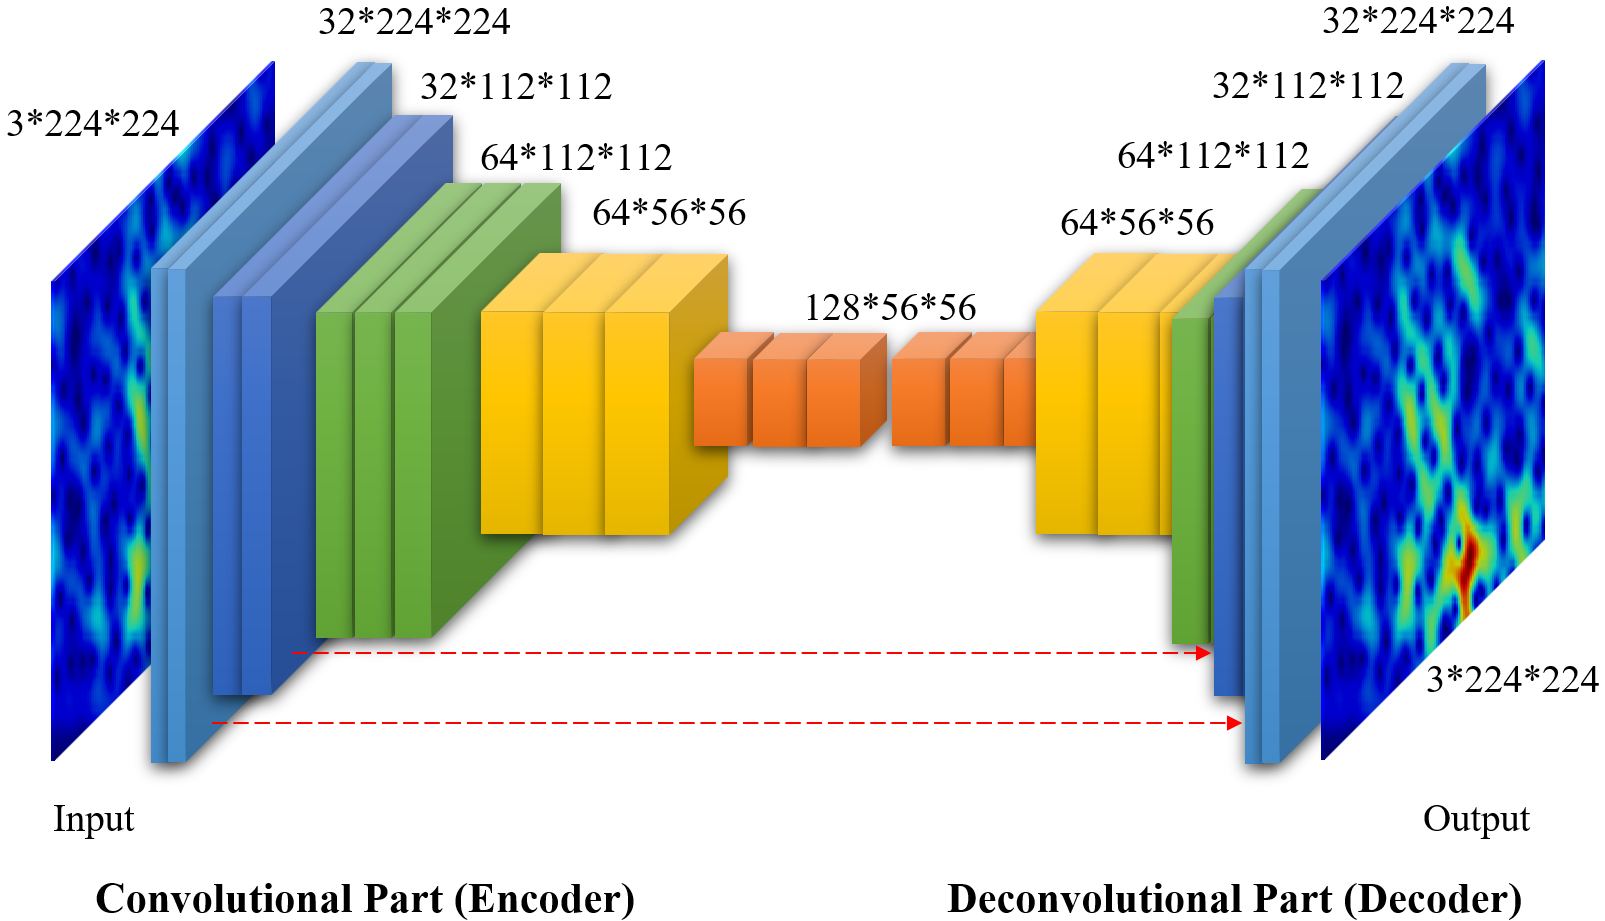
\includegraphics[width=0.48\textwidth,keepaspectratio]{img/cae.png}}
\caption{Convolutional AutoEncoder of spectrograms.}
\label{fig:cae_interpolation}
\end{figure}


\begin{figure*}
\centering
{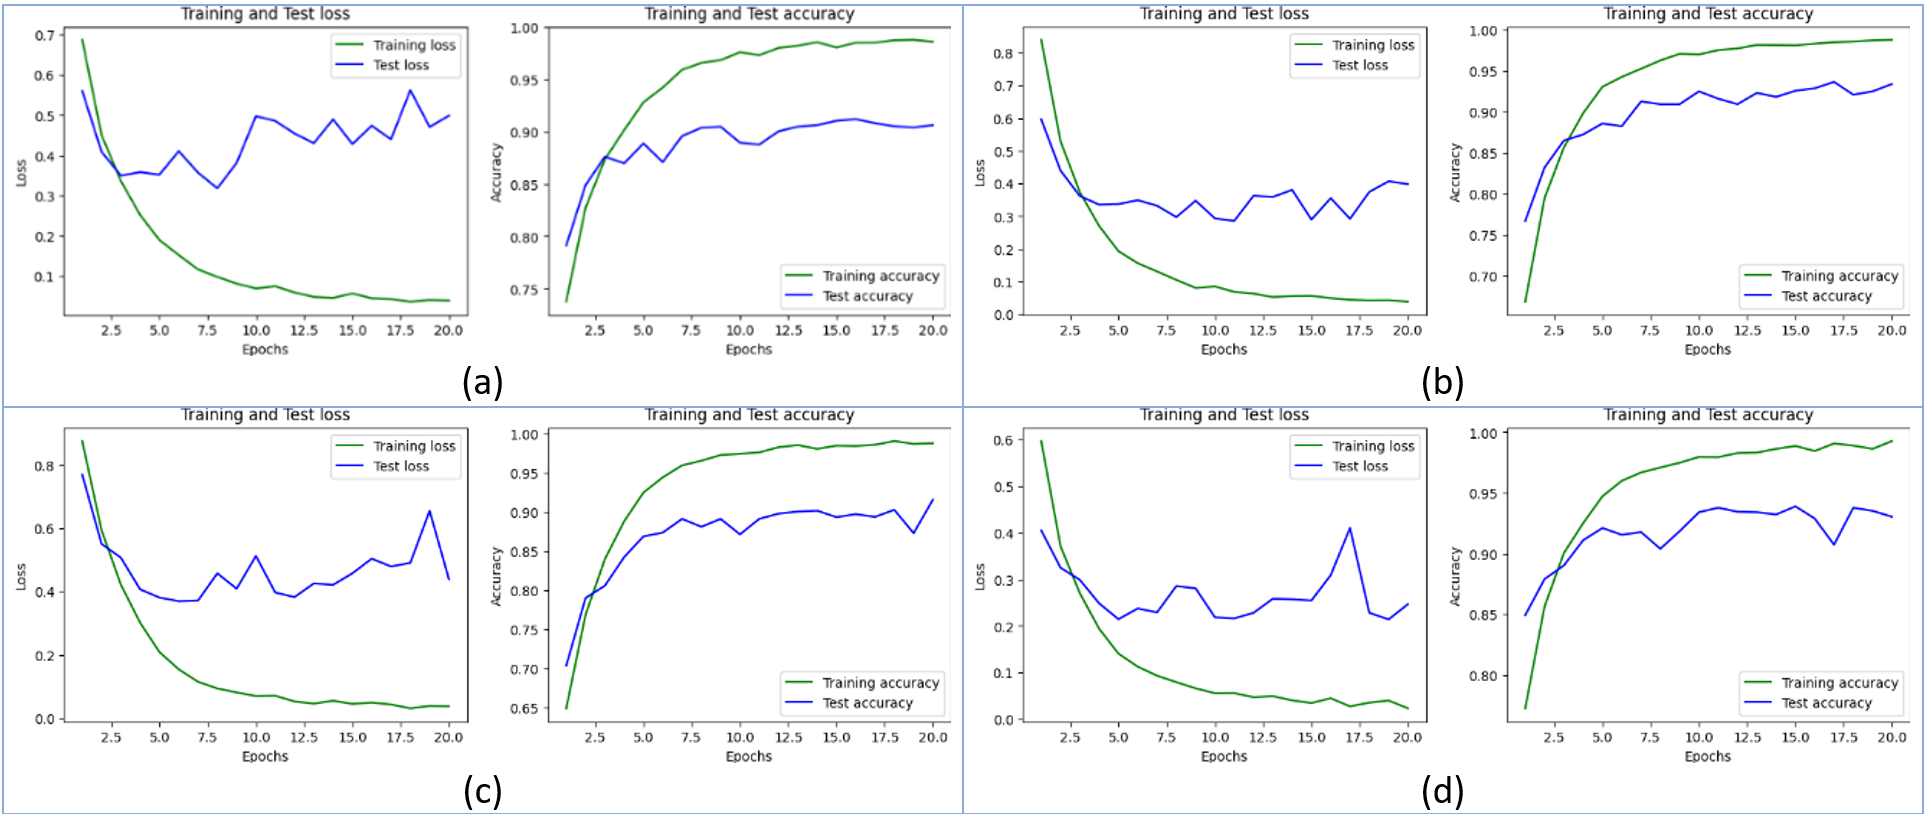
\includegraphics[width=0.8\textwidth,keepaspectratio]{img/curvas_entrenamiento.png}}
\caption{The training, and validation performance scores of the transfer learning using the AlexNet for the experiment: a) training and test loss for the experiment (viii), b) (ix), c) (xxi), and d) (xxv).}
\label{fig:da_training}
\end{figure*}
\begin{figure*}
\centering
{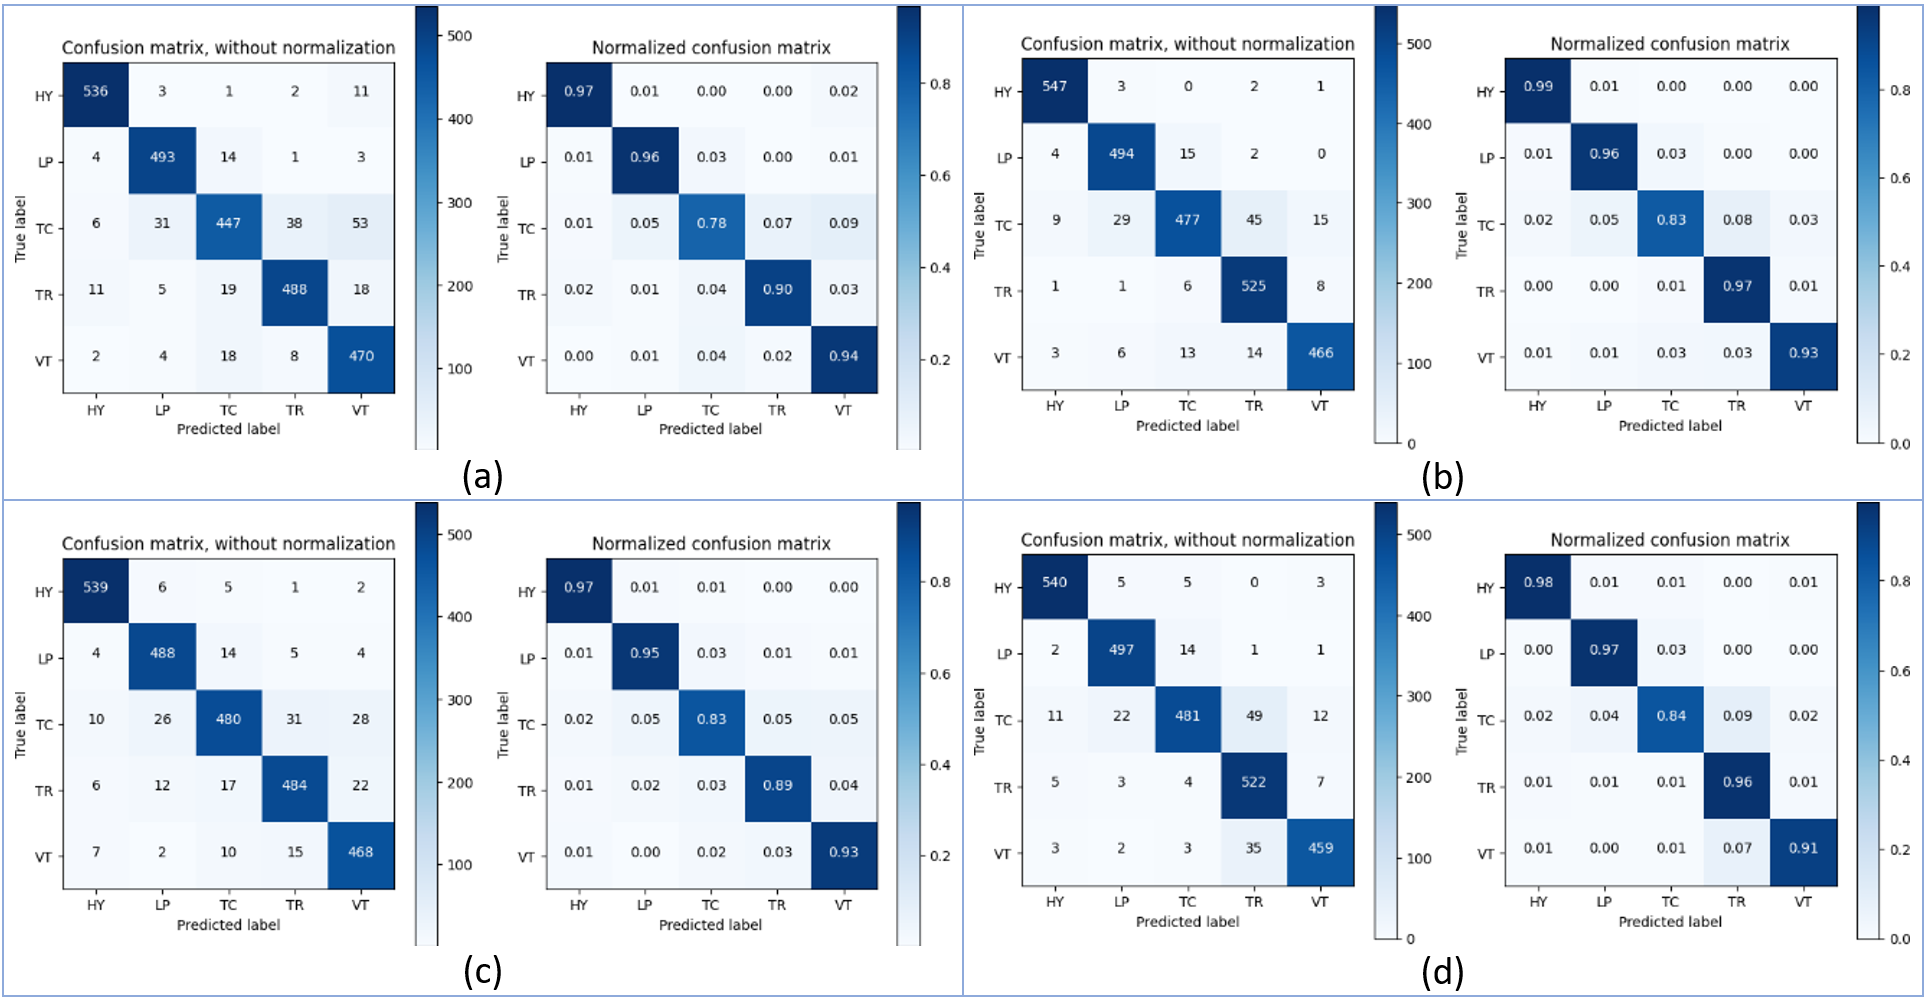
\includegraphics[width=0.8\textwidth,keepaspectratio]{img/matriz_confusion.png}}
\caption{Confusion matrix without normalization and normalized for experiments a) (viii), b) (ix), c) (xxi) and d) (xxv).}
\label{fig:da_confusion_matrix}
\end{figure*}

The experimental evidence underscores the importance of data augmentation techniques in enhancing the precision of deep learning models. Models trained without these data augmentation techniques exhibited low precision, as illustrated in Table \ref{table:training_statistic}.
To compare our models with the state-of-the-art, we considered performance metrics, including accuracy, precision, recall, specificity, and F1 score.
In the Table \ref{table:similarity_diversity_metrics}, the similarity metrics are calculated by comparing two datasets. Thus, there are two types of datasets:
\begin{itemize}
\item \textit{Real + augmented:} Since the VT event has enough examples and does not require augmented data to balance the dataset, these metrics were not calculated for this event due to a lack of comparison data.
\item \textit{Augmented:} Since all data is augmented, the comparison was made by dividing the dataset into two parts and comparing them.
\end{itemize}

\begin{table*}
\caption{Similarity and Diversity metrics for experimental datasets.}
\centering
\begin{adjustbox}{width=\textwidth}
\begin{tblr}{
  row{2} = {c},  cell{1}{1} = {r=2}{},  cell{1}{2} = {r=2}{},  cell{1}{3} = {c=6}{c},  cell{1}{9} = {c=6}{c},  cell{1}{15} = {c=6}{c},  cell{3}{3} = {r},  cell{3}{4} = {r},  cell{3}{5} = {r},  cell{3}{6} = {r},  cell{3}{7} = {r},  cell{3}{8} = {r},  cell{3}{9} = {r},  cell{3}{10} = {r},  cell{3}{11} = {r},  cell{3}{12} = {r},  cell{3}{13} = {r},  cell{3}{14} = {r},  cell{3}{15} = {r},  cell{3}{16} = {r},  cell{3}{17} = {r},  cell{3}{18} = {r},  cell{3}{19} = {r},  cell{3}{20} = {r},  cell{4}{3} = {r},  cell{4}{4} = {r},  cell{4}{5} = {r},  cell{4}{6} = {r},  cell{4}{7} = {r},  cell{4}{8} = {r},  cell{4}{9} = {r},  cell{4}{10} = {r},  cell{4}{11} = {r},  cell{4}{12} = {r},  
  cell{4}{13} = {r},  cell{4}{14} = {r},  cell{4}{15} = {r},  cell{4}{16} = {r},  cell{4}{17} = {r},  cell{4}{18} = {r},  cell{4}{19} = {r},  cell{4}{20} = {r},  cell{5}{3} = {r},  cell{5}{4} = {r},  cell{5}{5} = {r},  cell{5}{6} = {r},  cell{5}{7} = {r},  cell{5}{8} = {r},  cell{5}{9} = {r},  cell{5}{10} = {r},  cell{5}{11} = {r},  cell{5}{12} = {r},  cell{5}{13} = {r},  cell{5}{14} = {r},  cell{5}{15} = {r},  cell{5}{16} = {r},  cell{5}{17} = {r},  cell{5}{18} = {r},  cell{5}{19} = {r},  cell{5}{20} = {r},  cell{6}{3} = {r},  cell{6}{4} = {r},  
  cell{6}{5} = {r},  cell{6}{6} = {r},  cell{6}{7} = {r},  cell{6}{8} = {r},  cell{6}{9} = {r},  cell{6}{10} = {r},  cell{6}{11} = {r},  cell{6}{12} = {r},  cell{6}{13} = {r},  cell{6}{14} = {r},  cell{6}{15} = {r},  cell{6}{16} = {r},  cell{6}{17} = {r},  cell{6}{18} = {r},  cell{6}{19} = {r},  cell{6}{20} = {r},  cell{7}{3} = {r},  cell{7}{4} = {r},  cell{7}{5} = {r},  cell{7}{6} = {r},  cell{7}{7} = {r},  cell{7}{8} = {r},  cell{7}{9} = {r},  cell{7}{10} = {r},  cell{7}{11} = {r},  cell{7}{12} = {r},  cell{7}{13} = {r},  cell{7}{14} = {r},  cell{7}{15} = {r},  cell{7}{16} = {r},  cell{7}{17} = {r},  cell{7}{18} = {r},  cell{7}{19} = {r},  cell{7}{20} = {r},  cell{8}{3} = {r},  
  cell{8}{4} = {r},  cell{8}{5} = {r},  cell{8}{6} = {r},  cell{8}{7} = {r},  cell{8}{8} = {r},  cell{8}{9} = {r},  cell{8}{10} = {r},  cell{8}{11} = {r},  cell{8}{12} = {r},  cell{8}{13} = {r},  cell{8}{14} = {r},  cell{8}{15} = {r},  cell{8}{16} = {r},  cell{8}{17} = {r},  cell{8}{18} = {r},  cell{8}{19} = {r},  cell{8}{20} = {r},  cell{9}{3} = {r},  cell{9}{4} = {r},  cell{9}{5} = {r},  cell{9}{6} = {r},  cell{9}{7} = {r},  cell{9}{8} = {r},  cell{9}{9} = {r},  cell{9}{10} = {r},  cell{9}{11} = {r},  cell{9}{12} = {r},  cell{9}{13} = {r},  
  cell{9}{14} = {r},  cell{9}{15} = {r},  cell{9}{16} = {r},  cell{9}{17} = {r},  cell{9}{18} = {r},  cell{9}{19} = {r},  cell{9}{20} = {r},  cell{10}{3} = {r},  cell{10}{4} = {r},  cell{10}{5} = {r},  cell{10}{6} = {r},  cell{10}{7} = {r},  cell{10}{8} = {r},  cell{10}{9} = {r},  cell{10}{10} = {r},  cell{10}{11} = {r},  cell{10}{12} = {r},  cell{10}{13} = {r},  cell{10}{14} = {r},  cell{10}{15} = {r},  cell{10}{16} = {r},  cell{10}{17} = {r},  cell{10}{18} = {r},  cell{10}{19} = {r},  cell{10}{20} = {r},  cell{11}{3} = {r},  cell{11}{4} = {r},  cell{11}{5} = {r},  
  cell{11}{6} = {r},  cell{11}{7} = {r},  cell{11}{8} = {r},  cell{11}{9} = {r},  cell{11}{10} = {r},  cell{11}{11} = {r},  cell{11}{12} = {r},  cell{11}{13} = {r},  cell{11}{14} = {r},  cell{11}{15} = {r},  cell{11}{16} = {r},  cell{11}{17} = {r},  cell{11}{18} = {r},  cell{11}{19} = {r},  cell{11}{20} = {r},  cell{12}{3} = {r},  cell{12}{4} = {r},  cell{12}{5} = {r},  cell{12}{6} = {r},  cell{12}{7} = {r},  cell{12}{8} = {r},  cell{12}{9} = {r},  cell{12}{10} = {r},  cell{12}{11} = {r},  cell{12}{12} = {r},  cell{12}{13} = {r},  cell{12}{14} = {r},  cell{12}{15} = {r},  
  cell{12}{16} = {r},  cell{12}{17} = {r},  cell{12}{18} = {r},  cell{12}{19} = {r},  cell{12}{20} = {r},  cell{13}{3} = {r},  cell{13}{4} = {r},  cell{13}{5} = {r},  cell{13}{6} = {r},  cell{13}{7} = {r},  cell{13}{8} = {r},  cell{13}{9} = {r},  cell{13}{10} = {r},  cell{13}{11} = {r},  cell{13}{12} = {r},  cell{13}{13} = {r},  cell{13}{14} = {r},  cell{13}{15} = {r},  cell{13}{16} = {r},  cell{13}{17} = {r},  cell{13}{18} = {r},  cell{13}{19} = {r},  cell{13}{20} = {r},  cell{14}{3} = {r},  cell{14}{4} = {r},  cell{14}{5} = {r},  cell{14}{6} = {r},  cell{14}{7} = {r},  
  cell{14}{8} = {r},  cell{14}{9} = {r},  cell{14}{10} = {r},  cell{14}{11} = {r},  cell{14}{12} = {r},  cell{14}{13} = {r},  cell{14}{14} = {r},  cell{14}{15} = {r},  cell{14}{16} = {r},  cell{14}{17} = {r},  cell{14}{18} = {r},  cell{14}{19} = {r},  cell{14}{20} = {r},  cell{15}{3} = {r},  cell{15}{4} = {r},  cell{15}{5} = {r},  cell{15}{6} = {r},  cell{15}{7} = {r},  cell{15}{8} = {r},  cell{15}{9} = {r},  cell{15}{10} = {r},  cell{15}{11} = {r},  cell{15}{12} = {r},  cell{15}{13} = {r},  cell{15}{14} = {r},  cell{15}{15} = {r},  cell{15}{16} = {r},  cell{15}{17} = {r},  
  cell{15}{18} = {r},  cell{15}{19} = {r},  cell{15}{20} = {r},  cell{16}{3} = {r},  cell{16}{4} = {r},  cell{16}{5} = {r},  cell{16}{6} = {r},  cell{16}{7} = {r},  cell{16}{8} = {r},  cell{16}{9} = {r},  cell{16}{10} = {r},  cell{16}{11} = {r},  cell{16}{12} = {r},  cell{16}{13} = {r},  cell{16}{14} = {r},  cell{16}{15} = {r},  cell{16}{16} = {r},  cell{16}{17} = {r},  cell{16}{18} = {r},  cell{16}{19} = {r},  cell{16}{20} = {r},  
  cell{17}{3} = {r},  cell{17}{4} = {r},  cell{17}{5} = {r},  cell{17}{6} = {r},  cell{17}{7} = {r},  cell{17}{8} = {r},  cell{17}{9} = {r},  cell{17}{10} = {r},  cell{17}{11} = {r},  cell{17}{12} = {r},  cell{17}{13} = {r},  cell{17}{14} = {r},  cell{17}{15} = {r},  cell{17}{16} = {r},  cell{17}{17} = {r},  cell{17}{18} = {r},  cell{17}{19} = {r},  cell{17}{20} = {r},  cell{18}{3} = {r},  cell{18}{4} = {r},  cell{18}{5} = {r},  cell{18}{6} = {r},  cell{18}{7} = {r},  cell{18}{8} = {r},  cell{18}{9} = {r},  cell{18}{10} = {r},  cell{18}{11} = {r},  cell{18}{12} = {r},  
  cell{18}{13} = {r},  cell{18}{14} = {r},  cell{18}{15} = {r},  cell{18}{16} = {r},  cell{18}{17} = {r},  cell{18}{18} = {r},  cell{18}{19} = {r},  cell{18}{20} = {r},  cell{19}{3} = {r},  cell{19}{4} = {r},  cell{19}{5} = {r},  cell{19}{6} = {r},  cell{19}{7} = {r},  cell{19}{8} = {r},  cell{19}{9} = {r},  cell{19}{10} = {r},  cell{19}{11} = {r},  cell{19}{12} = {r},  cell{19}{13} = {r},  cell{19}{14} = {r},  cell{19}{15} = {r},  
  cell{19}{16} = {r},  cell{19}{17} = {r},  cell{19}{18} = {r},  cell{19}{19} = {r},  cell{19}{20} = {r},  cell{20}{3} = {r},  cell{20}{4} = {r},  cell{20}{5} = {r},  cell{20}{6} = {r},  cell{20}{7} = {r},  cell{20}{8} = {r},  cell{20}{9} = {r},  cell{20}{10} = {r},  cell{20}{11} = {r},  cell{20}{12} = {r},  cell{20}{13} = {r},  cell{20}{14} = {r},  cell{20}{15} = {r},  cell{20}{16} = {r},  cell{20}{17} = {r},  cell{20}{18} = {r},  
  cell{20}{19} = {r},  cell{20}{20} = {r},  cell{21}{3} = {r},  cell{21}{4} = {r},  cell{21}{5} = {r},  cell{21}{6} = {r},  cell{21}{7} = {r},  cell{21}{8} = {r},  cell{21}{9} = {r},  cell{21}{10} = {r},  cell{21}{11} = {r},  cell{21}{12} = {r},  cell{21}{13} = {r},  cell{21}{14} = {r},  cell{21}{15} = {r},  cell{21}{16} = {r},  cell{21}{17} = {r},  cell{21}{18} = {r},  cell{21}{19} = {r},  cell{21}{20} = {r},  cell{22}{3} = {r},  cell{22}{4} = {r},  cell{22}{5} = {r},  cell{22}{6} = {r},  cell{22}{7} = {r},  cell{22}{8} = {r},  cell{22}{9} = {r},  cell{22}{10} = {r},  
  cell{22}{11} = {r},  cell{22}{12} = {r},  cell{22}{13} = {r},  cell{22}{14} = {r},  cell{22}{15} = {r},  cell{22}{16} = {r},  cell{22}{17} = {r},  cell{22}{18} = {r},  cell{22}{19} = {r},  cell{22}{20} = {r},  cell{23}{3} = {r},  cell{23}{4} = {r},  cell{23}{5} = {r},  cell{23}{6} = {r},  cell{23}{7} = {r},  cell{23}{8} = {r},  cell{23}{9} = {r},  cell{23}{10} = {r},  cell{23}{11} = {r},  cell{23}{12} = {r},  cell{23}{13} = {r},  cell{23}{14} = {r},  cell{23}{15} = {r},  cell{23}{16} = {r},  cell{23}{17} = {r},  cell{23}{18} = {r},  cell{23}{19} = {r},  cell{23}{20} = {r},  
  cell{24}{3} = {r},  cell{24}{4} = {r},  cell{24}{5} = {r},  cell{24}{6} = {r},  cell{24}{7} = {r},  cell{24}{8} = {r},  cell{24}{9} = {r},  cell{24}{10} = {r},  cell{24}{11} = {r},  cell{24}{12} = {r},  cell{24}{13} = {r},  cell{24}{14} = {r},  cell{24}{15} = {r},  cell{24}{16} = {r},  cell{24}{17} = {r},  cell{24}{18} = {r},  cell{24}{19} = {r},  cell{24}{20} = {r},  cell{25}{3} = {r},  cell{25}{4} = {r},  cell{25}{5} = {r},  cell{25}{6} = {r},  cell{25}{7} = {r},  cell{25}{8} = {r},  cell{25}{9} = {r},  cell{25}{10} = {r},  cell{25}{11} = {r},  cell{25}{12} = {r},  
  cell{25}{13} = {r},  cell{25}{14} = {r},  cell{25}{15} = {r},  cell{25}{16} = {r},  cell{25}{17} = {r},  cell{25}{18} = {r},  cell{25}{19} = {r},  cell{25}{20} = {r},  cell{26}{3} = {r},  cell{26}{4} = {r},  cell{26}{5} = {r},  cell{26}{6} = {r},  cell{26}{7} = {r},  cell{26}{8} = {r},  cell{26}{9} = {r},  cell{26}{10} = {r},  cell{26}{11} = {r},  cell{26}{12} = {r},  cell{26}{13} = {r},  cell{26}{14} = {r},  cell{26}{15} = {r},  
  cell{26}{16} = {r},  cell{26}{17} = {r},  cell{26}{18} = {r},  cell{26}{19} = {r},  cell{26}{20} = {r},  cell{27}{3} = {r},  cell{27}{4} = {r},  cell{27}{5} = {r},  cell{27}{6} = {r},  cell{27}{7} = {r},  cell{27}{8} = {r},  cell{27}{9} = {r},  cell{27}{10} = {r},  cell{27}{11} = {r},  cell{27}{12} = {r},  cell{27}{13} = {r},  cell{27}{14} = {r},  cell{27}{15} = {r},  cell{27}{16} = {r},  cell{27}{17} = {r},  cell{27}{18} = {r},  cell{27}{19} = {r},  cell{27}{20} = {r},
}
\hline\hline %inserts double horizontal lines
Dataset & Data augmentation & {Fréchet Inception Distance\\(FID)
       } &  &  &  &  &  & {Kernel Inception Distance\\(KID)
       } &  &  &  &  &  & {Multiscale Structural Similarity Index\\(MS-SSIM)} &  &  &  &  & \\
\hline % inserts single horizontal line
 &  & HY & LP & TC & TR & VT & FID & HY & LP & TC & TR & VT & KID & HY & LP & TC & TR & VT & MS\\
\hline % inserts single horizontal line
(i) & No & 0.16 & 0.10 & 0.02 & 0.05 & 0.02 & 0.03 & 0.14 & -0.75 & 3.78 & 0.31 & -0.23 & 1.21 & 0.34 & 0.41 & 0.33 & 0.29 & 0.34 & 0.34\\
(ii) & Rotation(5\%-25\%) & 0.70 & 0.61 & 0.50 & 0.45 & ~ & 0.56 & 4.81 & -1.40 & 4.41 & 2.56 & ~ & 2.59 & 0.38 & 0.42 & 0.36 & 0.29 & ~ & 0.36\\
(iii) & Rotation(5\%-25\%) & 0.03 & 0.01 & 0.04 & 0.02 & 0.03 & 0.02 & 1.62 & 0.15 & 1.16 & -1.03 & 2.34 & 0.85 & 0.36 & 0.42 & 0.36 & 0.33 & 0.35 & 0.37\\
(iv) & Jittering(0.2) & 10.09 & 5.46 & 7.65 & 8.88 & ~ & 8.02 & 56.99 & 18.80 & 40.98 & 48.72 & ~ & 41.37 & 0.28 & 0.36 & 0.27 & 0.26 & ~ & 0.29\\
(v) & Jittering(0.2) & 0.01 & 0.01 & 0.02 & 0.02 & 0.03 & 0.02 & -2.50 & -2.35 & 3.38 & 0.24 & -2.77 & -0.80 & 0.26 & 0.33 & 0.26 & 0.21 & 0.23 & 0.26\\
(vi) & Drifting Drift(0.01-0.1) & 34.80 & 30.48 & 35.93 & 30.01 & ~ & 32.81 & 102.53 & 71.83 & 89.02 & 83.60 & ~ & 86.75 & 0.40 & 0.46 & 0.42 & 0.35 & ~ & 0.41\\
(vii) & Drifting Drift(0.01-0.1) & 0.01 & 0.02 & 0.01 & 0.01 & 0.01 & 0.01 & -0.06 & -0.10 & 0.29 & 0.51 & -0.11 & 0.11 & 0.80 & 0.81 & 0.81 & 0.76 & 0.71 & 0.78\\
(viii) & Drifting Drift(0.001-0.01) & 1.50 & 1.23 & 2.69 & 0.84 & ~ & 1.56 & 3.25 & 3.61 & 3.84 & 1.01 & ~ & 2.93 & 0.37 & 0.42 & 0.38 & 0.31 & ~ & 0.37\\
(ix) & Drifting Drift(0.001-0.01) & 0.03 & 0.01 & 0.02 & 0.03 & 0.01 & 0.02 & 1.53 & -1.02 & 0.30 & 1.14 & -0.80 & 0.23 & 0.42 & 0.48 & 0.43 & 0.37 & 0.36 & 0.41\\
(x) & Drifting Drift(0.0001-0.001) & 0.02 & 0.02 & 0.03 & 0.02 & ~ & 0.02 & -4.42 & 4.68 & -3.96 & 0.79 & ~ & -0.73 & 0.35 & 0.40 & 0.33 & 0.29 & ~ & 0.34\\
(xi) & Drifting Drift(0.0001-0.001) & 0.01 & 0.01 & 0.02 & 0.01 & 0.01 & 0.01 & -5.60 & -1.65 & 2.42 & 3.00 & 1.74 & -0.02 & 0.35 & 0.40 & 0.32 & 0.31 & 0.34 & 0.34\\
(xii) & Genetic Algorithm Segment
  Size(5s) Crossover Segments(3) & 0.89 & 0.41 & 0.39 & 0.28 & ~ & 0.49 & 2.36 & 2.98 & -1.94 & 2.55 & ~ & 1.49 & 0.38 & 0.40 & 0.35 & 0.30 & ~ & 0.36\\
(xiii) & Genetic
  Algorithm Segment Size(5s) Crossover Segments(3) & 0.02 & 0.01 & 0.00 & 0.01 & 0.01 & 0.01 & 0.45 & -2.49 & -0.40 & -2.06 & 2.54 & -0.39 & 0.35 & 0.40 & 0.37 & 0.30 & 0.36 & 0.36\\
(xiv) & Genetic Algorithm Segment
  Size(5s) Crossover Segments(5) & 1.65 & 0.83 & 0.76 & 1.03 & ~ & 1.07 & 1.51 & 4.59 & 2.90 & 1.29 & ~ & 2.57 & 0.35 & 0.41 & 0.35 & 0.30 & ~ & 0.35\\
(xv) & Genetic Algorithm
  Segment Size(5s) Crossover Segments(5) & 0.02 & 0.01 & 0.01 & 0.02 & 0.01 & 0.01 & 1.06 & -0.48 & -0.32 & -2.37 & -1.77 & -0.77 & 0.35 & 0.40 & 0.37 & 0.33 & 0.40 & 0.37\\
(xvi) & Genetic Algorithm Signal Percent(40\%) Crossover
  Segments(10) & 0.90 & 0.63 & 0.55 & 0.41 & ~ & 0.63 & 3.99 & 1.91 & 0.08 & 4.25 & ~ & 2.56 & 0.36 & 0.41 & 0.35 & 0.30 & ~ & 0.35\\
(xvii) & Genetic Algorithm
  Signal Percent(40\%) Crossover Segments(10) & 0.02 & 0.02 & 0.04 & 0.01 & 0.01 & 0.02 & -0.28 & -3.37 & -0.14 & 1.87 & -0.70 & -0.52 & 0.34 & 0.41 & 0.32 & 0.29 & 0.34 & 0.34\\
(xviii) & Genetic Algorithm Signal Percent(45\%) Crossover
  Segments(10) & 0.97 & 0.67 & 0.73 & 0.36 & ~ & 0.68 & 4.43 & -0.28 & 3.54 & 0.97 & ~ & 2.16 & 0.35 & 0.41 & 0.33 & 0.30 & ~ & 0.35\\
(xix) & Genetic Algorithm
  Signal Percent(45\%) Crossover Segments(10) & 0.01 & 0.00 & 0.00 & 0.01 & 0.01 & 0.01 & 0.91 & 0.75 & -0.73 & 2.75 & 0.86 & 0.91 & 0.31 & 0.41 & 0.35 & 0.30 & 0.34 & 0.34\\
(xx) & SpecAugment Frequency Percent(0\%-10\%) Frequency
  Masks(2) Time Percent(0\%-10\%) Time Marks(2) & 1.53 & 1.48 & 1.85 & 1.21 & ~ & 1.52 & 6.23 & 4.41 & 6.33 & 2.06 & ~ & 4.76 & 0.37 & 0.41 & 0.33 & 0.30 & ~ & 0.35\\
(xxi) & SpecAugment
  Frequency Percent(0\%-10\%) Frequency Masks(2) Time Percent(0\%-10\%) Time
  Marks(2) & 0.00 & 0.01 & 0.02 & 0.01 & 0.01 & 0.01 & -1.21 & 2.46 & -0.33 & -1.04 & 1.03 & 0.18 & 0.34 & 0.40 & 0.35 & 0.31 & 0.34 & 0.35\\
(xxii) & SpecAugment Frequency Percent(0\%-15\%) Frequency
  Masks(2) Time Percent(0\%-15\%) Time Marks(2) & 3.84 & 3.45 & 3.08 & 3.22 & ~ & 3.40 & 16.73 & 11.34 & 7.82 & 6.15 & ~ & 10.51 & 0.35 & 0.41 & 0.33 & 0.31 & ~ & 0.35\\
(xxiii) & SpecAugment
  Frequency Percent(0\%-15\%) Frequency Masks(2) Time Percent(0\%-15\%) Time
  Marks(2) & 0.01 & 0.01 & 0.01 & 0.00 & 0.01 & 0.01 & 0.31 & 1.29 & 0.47 & 0.72 & -0.61 & 0.44 & 0.35 & 0.40 & 0.36 & 0.32 & 0.39 & 0.37\\
(xxiv) & Interpolation
  AE Signal percent(40\%-60\%) & 2.31 & 2.46 & 2.18 & 1.88 & ~ & 2.21 & 9.48 & 3.04 & 4.03 & 7.12 & ~ & 5.92 & 0.38 & 0.44 & 0.36 & 0.33 & ~ & 0.38\\
(xxv) & Interpolation AE Signal percent(40\%-60\%) & 0.01 & 0.01 & 0.01 & 0.01 & 0.01 & 0.01 & -0.22 & 0.62 & -0.89 & -0.44 & 0.03 & -0.18 & 0.43 & 0.48 & 0.41 & 0.37 & 0.41 & 0.42\\
\hline %inserts single line
\end{tblr}
\end{adjustbox}
\label{table:similarity_diversity_metrics}
\end{table*}

\begin{table*}
\caption{Relationship between Data Augmentation and Dataset.}
\centering
\begin{tabular}{clcc}
\hline\hline %inserts double horizontal lines  
  \multirow{2}{*}{Code} & \multirow{2}{*}{Data augmentation} & \multicolumn{2}{c}{ Datasets } \\
  \cline{3-4} % inserts single horizontal line
 &  & 
  Real + Augmented
   & 
  Augmented
   \\
\hline % inserts single horizontal line
N & Real dataset & i & ~ \\
R & Rotation (5\%-25\%) & ii & iii \\
J & Jittering (0.2) & iv & v \\
D & Drifting (0.01-0.1) & vi & vii \\
DD & Drifting (0.001-0.01) & viii & ix \\
DDD & Drifting (0.0001-0.001) & x & xi \\
G & Genetic Algorithm Segment Size(5s) Crossover Segments(3) & xii & xiii \\
GG & Genetic Algorithm Segment Size(5s) Crossover Segments(5) & xiv & xv \\
H & Genetic Algorithm Signal Percent(40\%) Crossover Segments(10) & xvi & xvii \\
HH & Genetic Algorithm Signal Percent(45\%) Crossover Segments(10) & xviii & xix \\
S & SpecAugment Frequency Percent(0\%-10\%) Frequency Masks(2) Time Percent(0\%-10\%) Time Marks(2) & xx & xxi \\
SS & SpecAugment Frequency Percent(0\%-15\%) Frequency Masks(2) Time Percent(0\%-15\%) Time Marks(2) & xxii & xxiii \\
I & Interpolation AE Signal percent(40\%-60\%) & xxiv & xv \\
\hline %inserts single line
\end{tabular}
\label{table:code_dataset}
\end{table*}


\begin{figure*}
\centering
{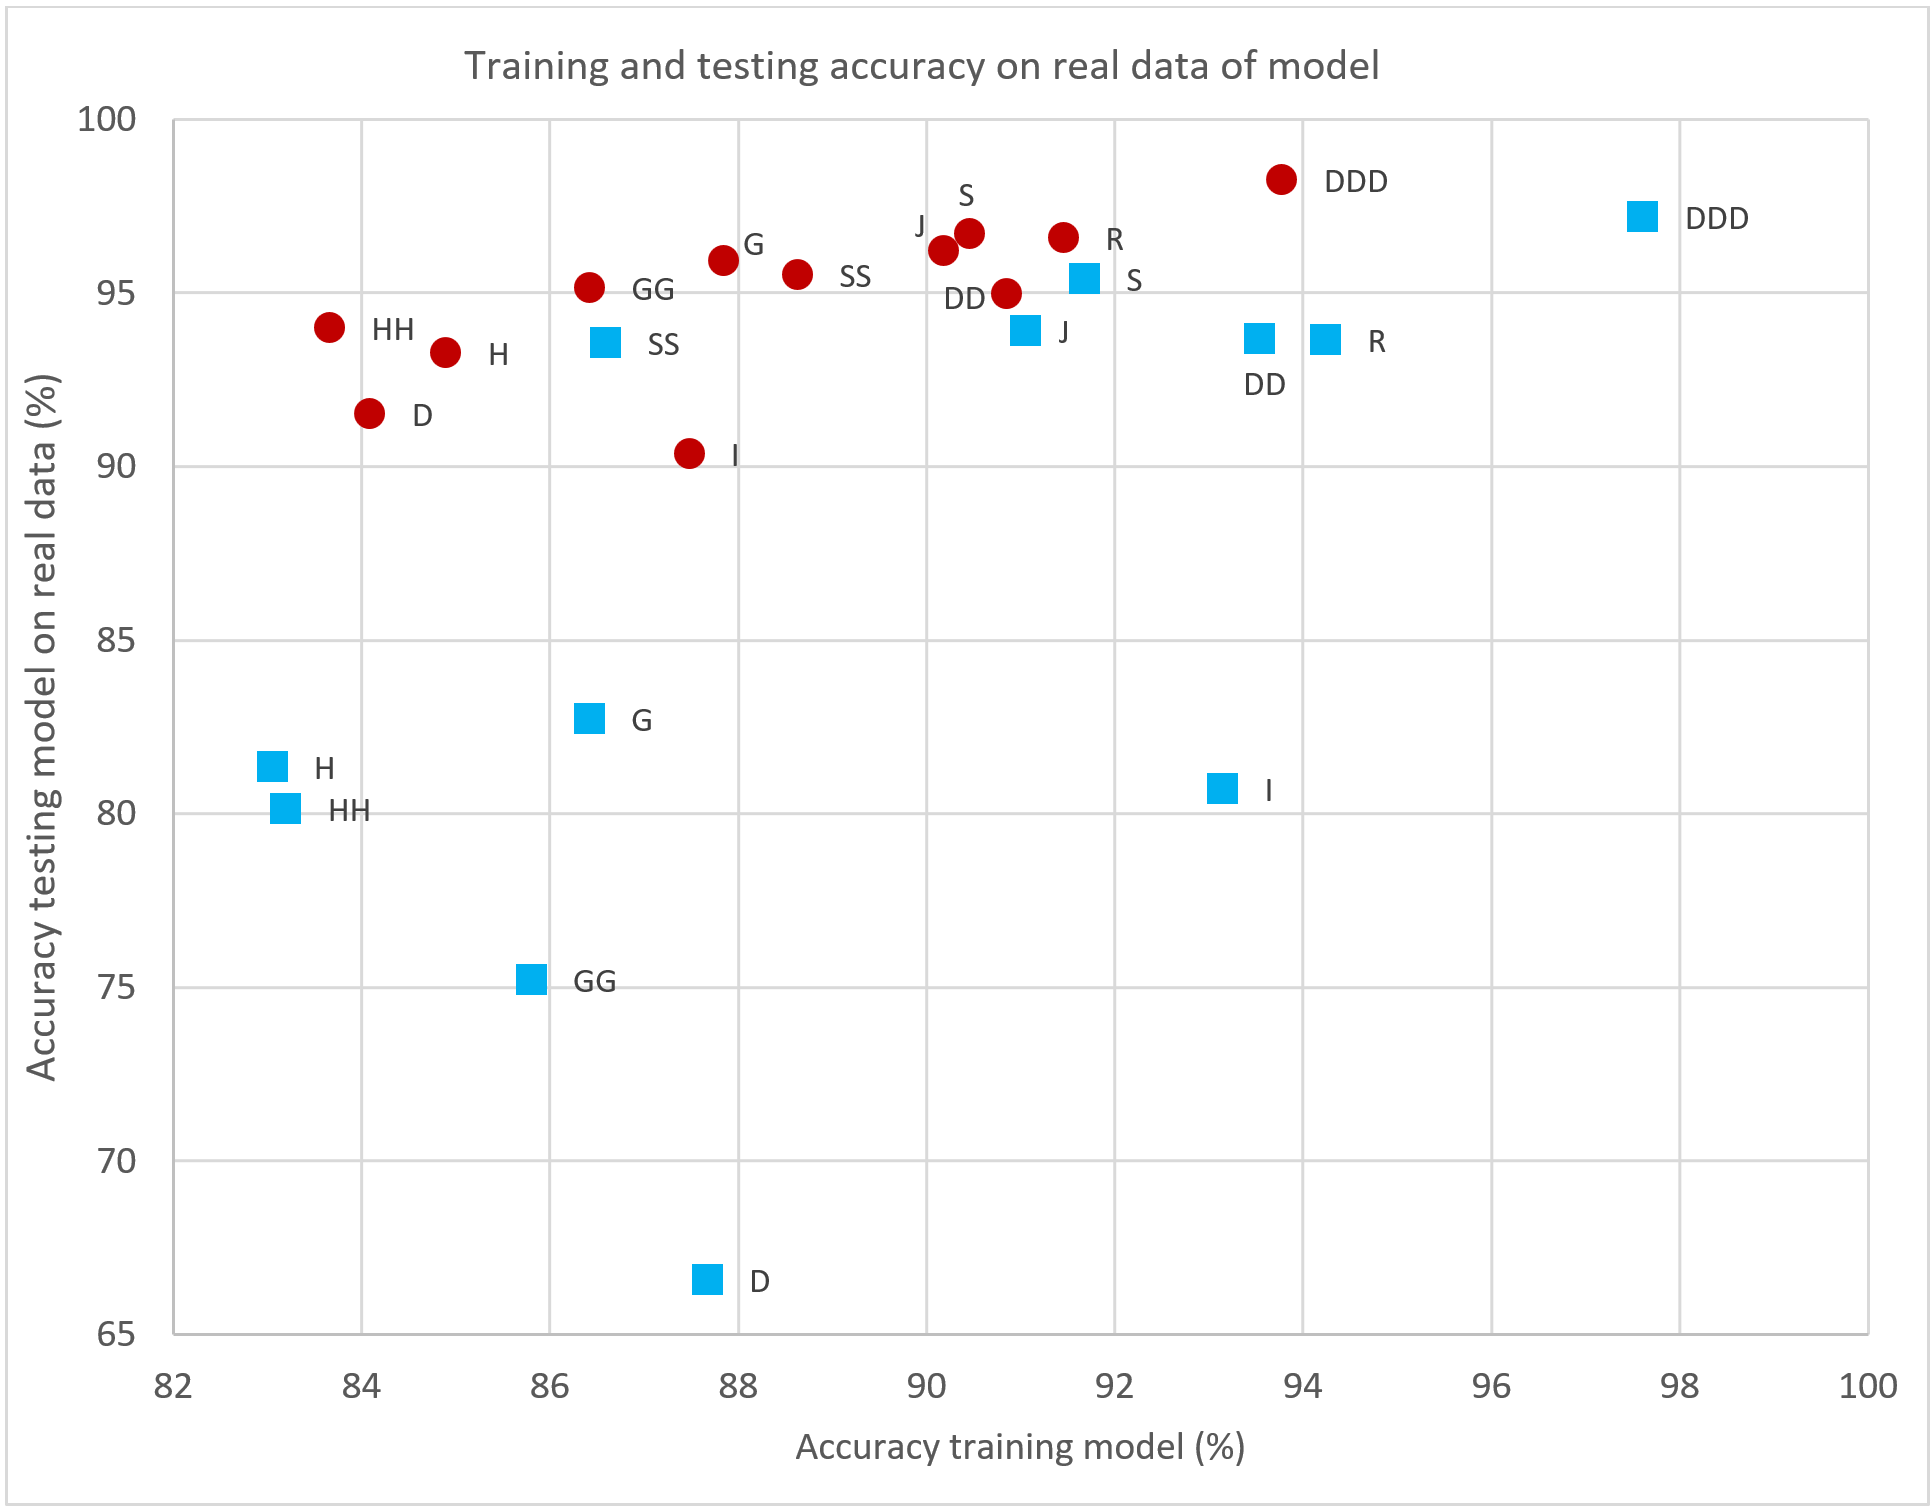
\includegraphics[width=0.7\textwidth,keepaspectratio]{img/entrenamiento_prueba.png}}
\caption{Accuracy of model training and testing on real data. \textcolor{dotgreen}{\textbf{Green}} shape indicates real dataset with 62.8\% of accuracy, \textcolor{dotred}{\textbf{red}} circles indicate datasets with real and augmented data, and \textcolor{dotsky}{\textbf{turquoise}} squares are entirely augmented datasets. The codes are described in Table \ref{table:code_dataset}.}
\label{fig:da_training_test}
\end{figure*}

\begin{figure*}
\centering
{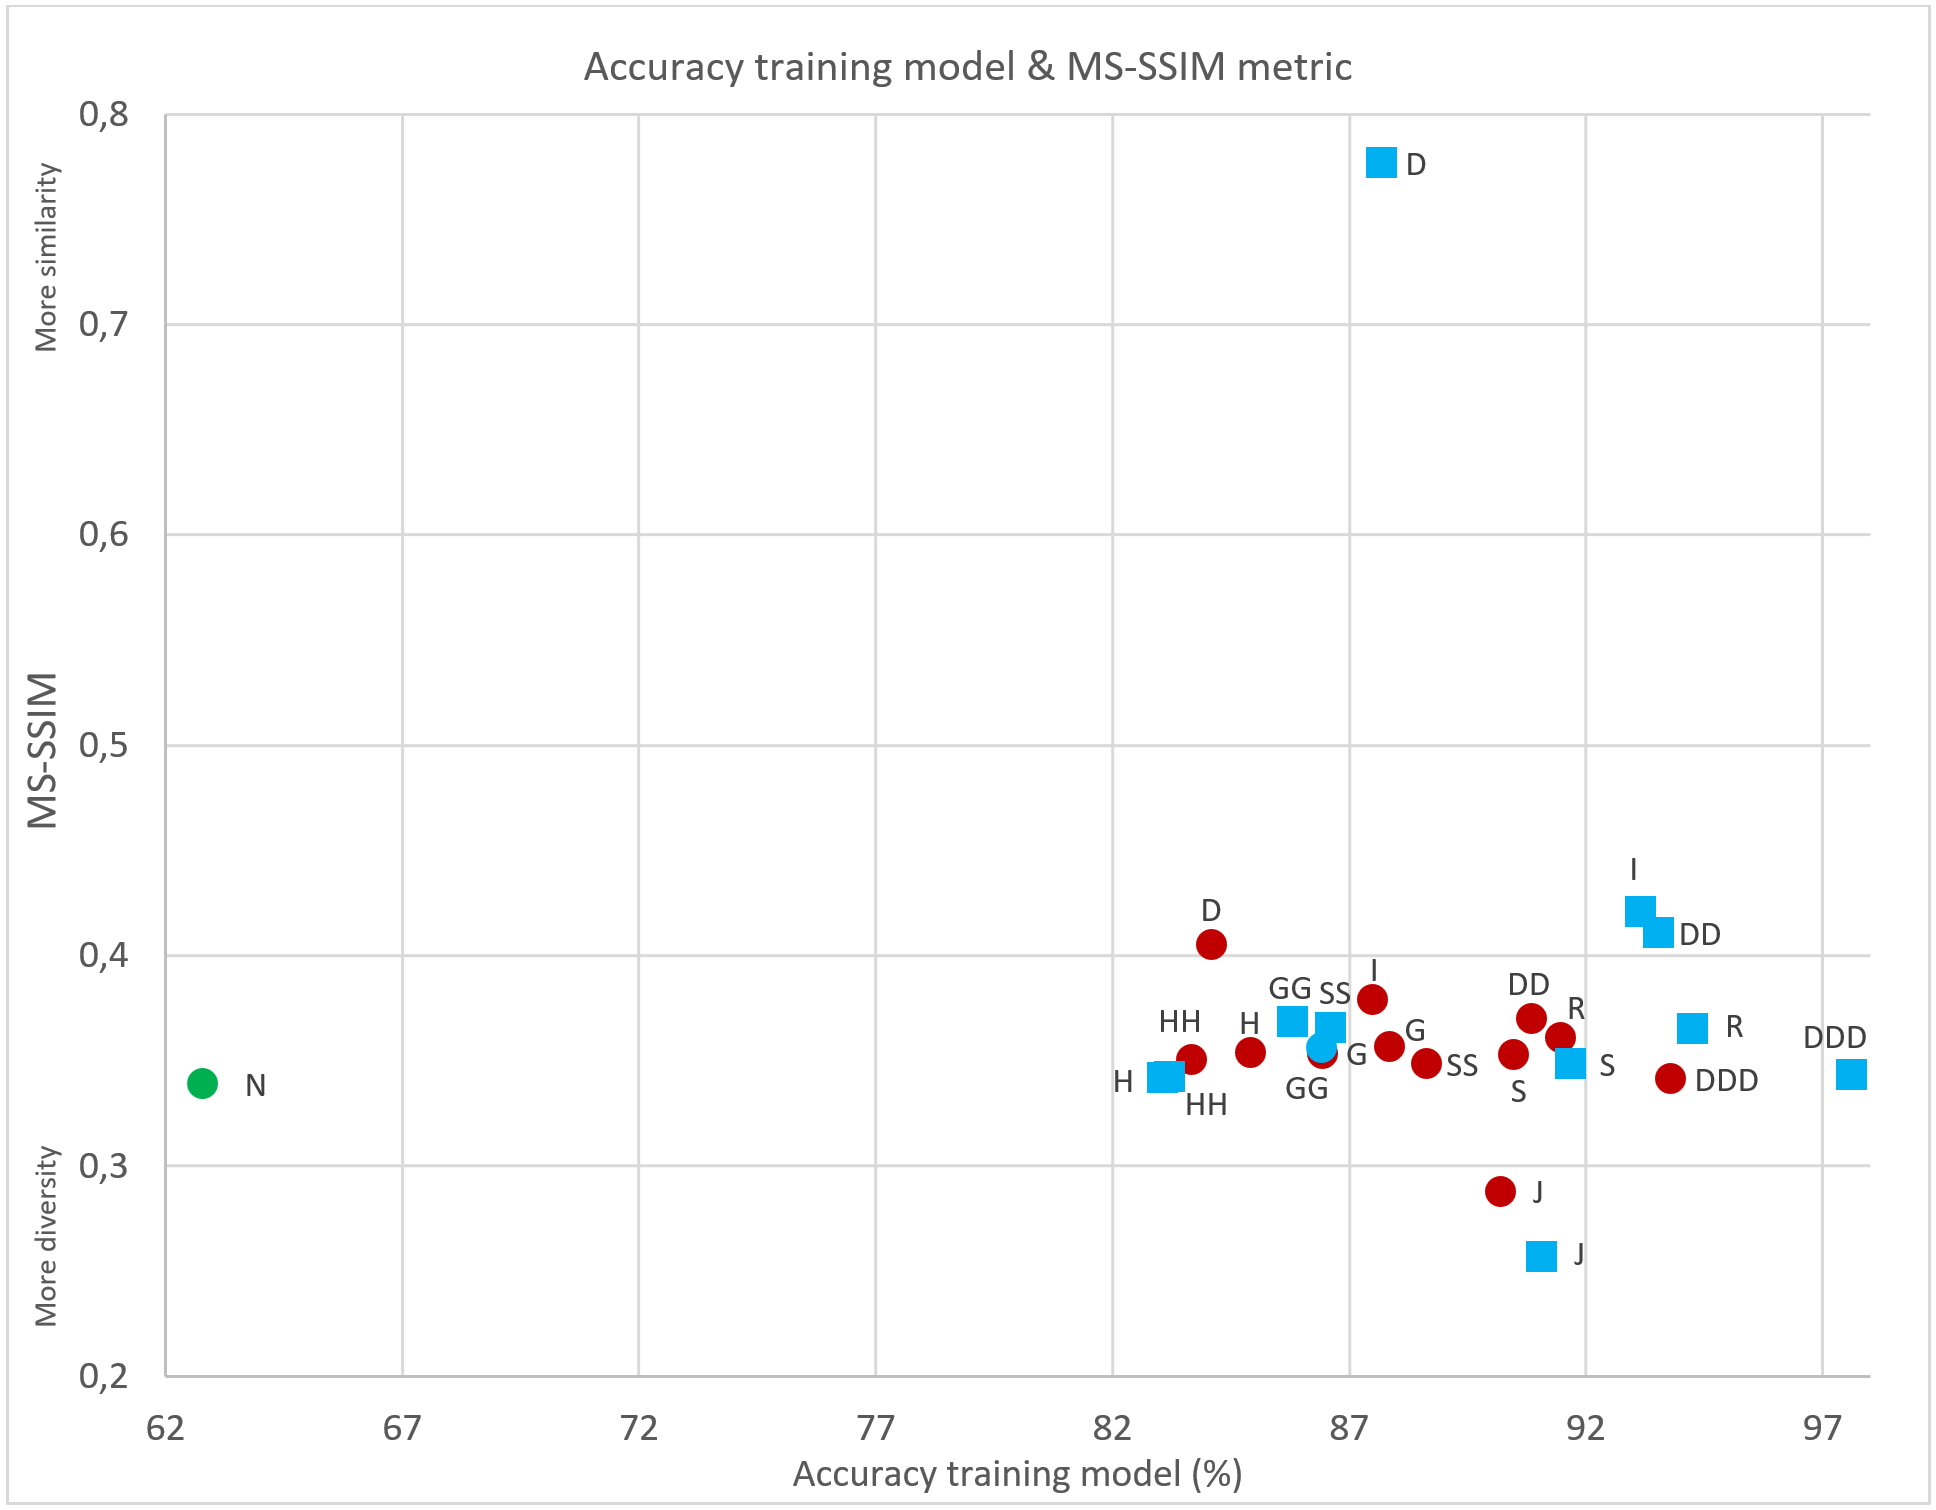
\includegraphics[width=0.7\textwidth,keepaspectratio]{img/entrenamiento_msssim.png}}
\caption{Accuracy of model training and MS-SSIM metric. \textcolor{dotgreen}{\textbf{Green}} shape indicates real dataset, \textcolor{dotred}{\textbf{red}} circles indicate datasets with real and augmented data, and \textcolor{dotsky}{\textbf{turquoise}} squares are entirely augmented datasets. The codes are described in Table \ref{table:code_dataset}.
}
\label{fig:da_training_msssim}
\end{figure*}

\begin{figure*}
\centering
{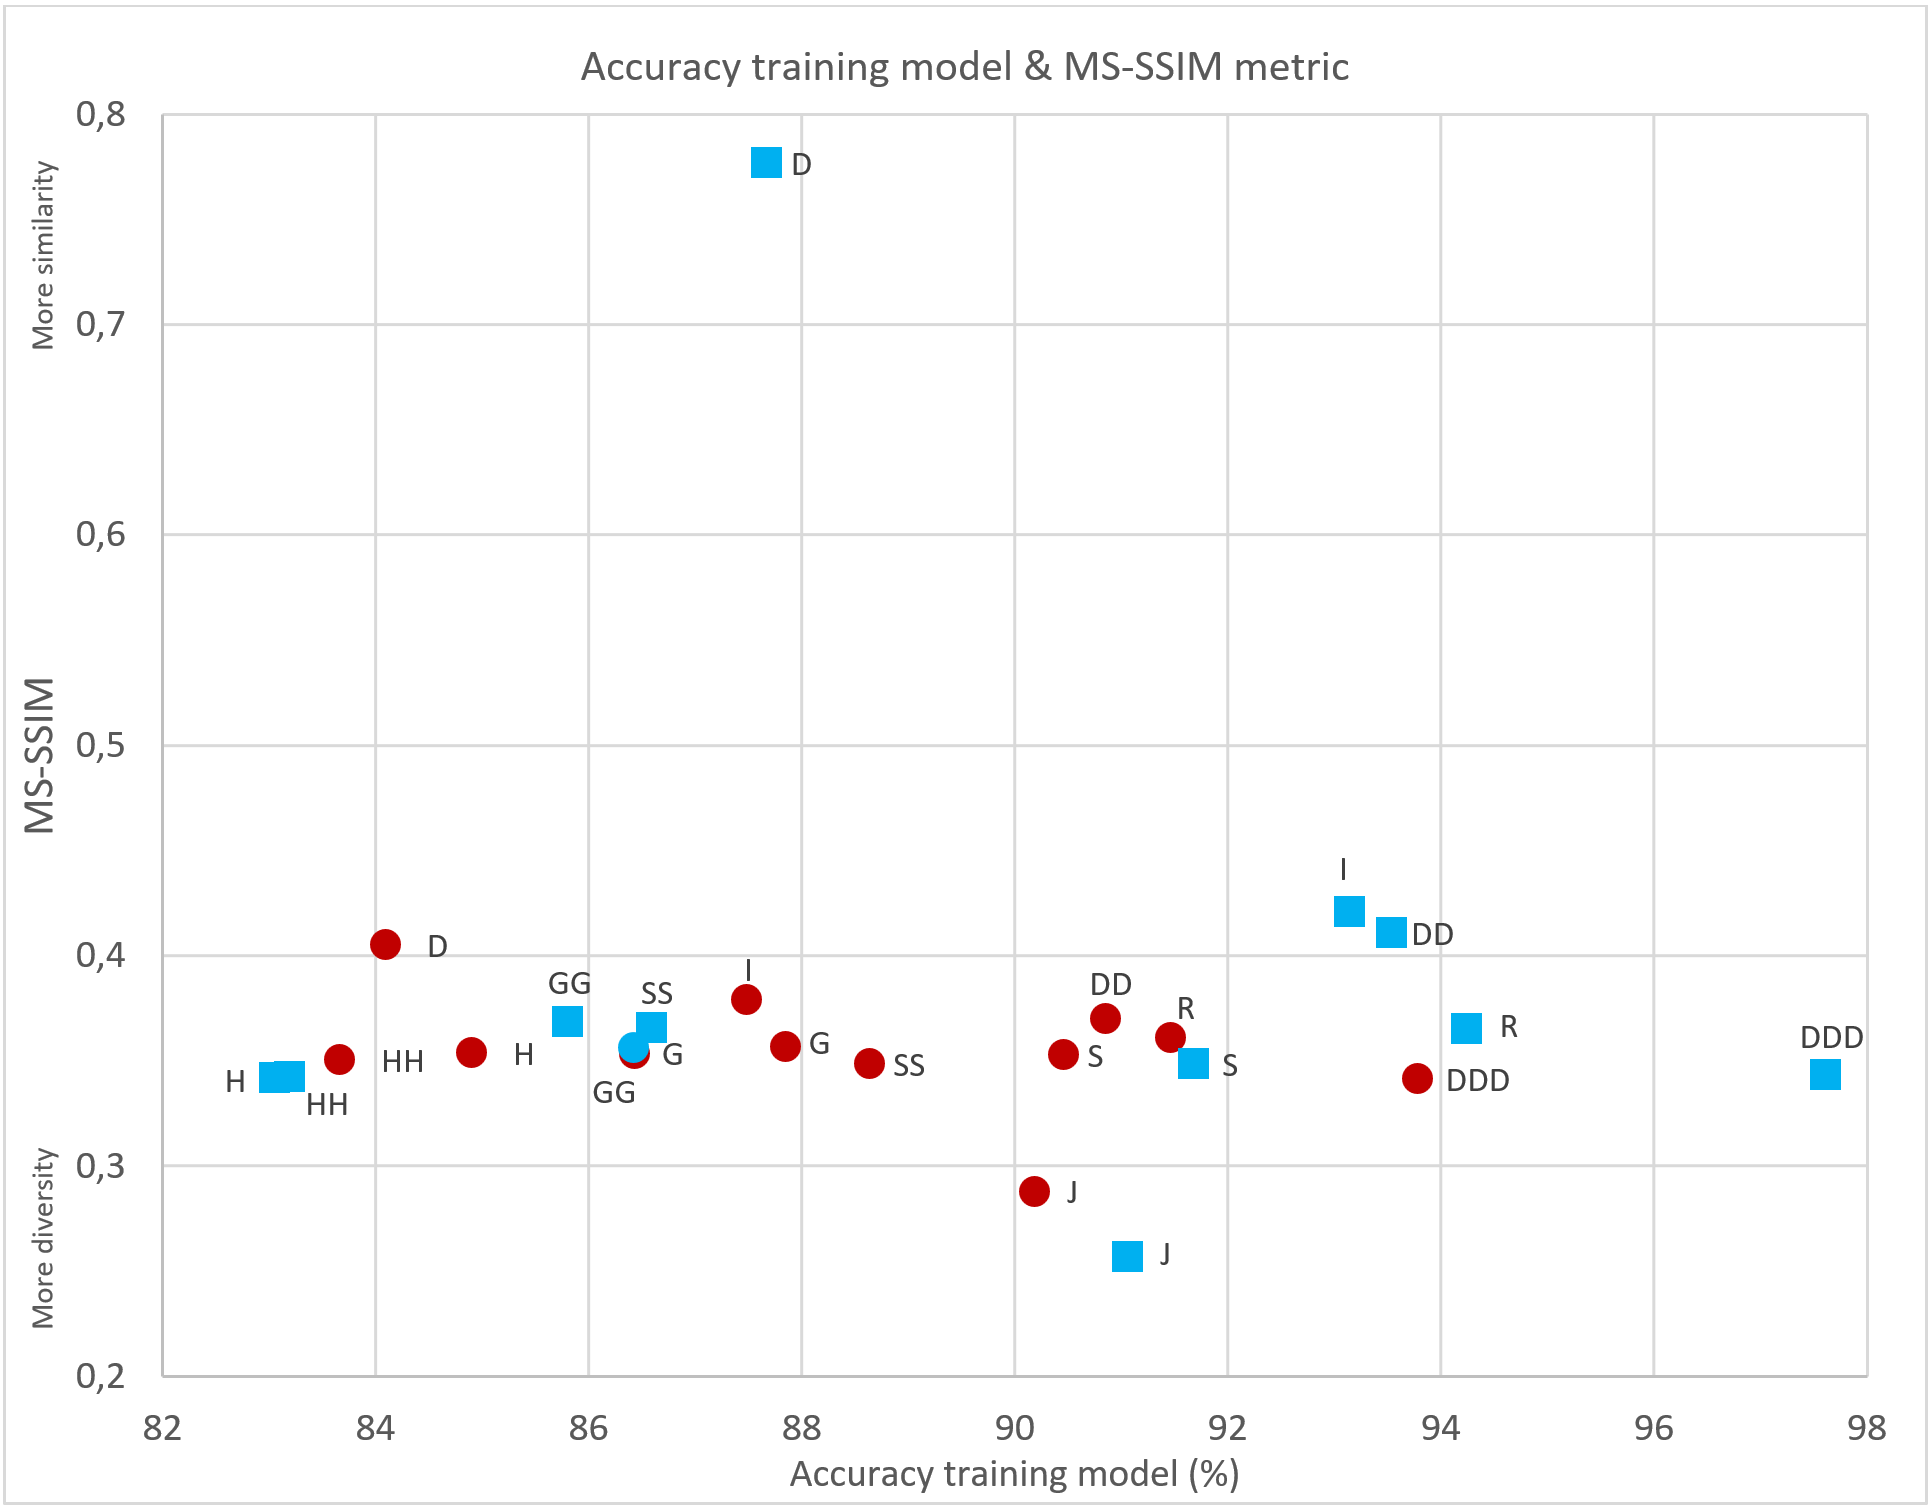
\includegraphics[width=0.7\textwidth,keepaspectratio]{img/entrenamiento_msssim_zoom.png}}
\caption{Zooming at figure of model training accuracy and MS-SSIM metric. \textcolor{dotgreen}{\textbf{Green}} shape indicates real dataset, \textcolor{dotred}{\textbf{red}} circles indicate datasets with real and augmented data, and \textcolor{dotsky}{\textbf{turquoise}} squares are entirely augmented datasets. The codes are described in Table \ref{table:code_dataset}.}
\label{fig:da_training_msssim_zoom}
\end{figure*}

\begin{figure*}
\centering
{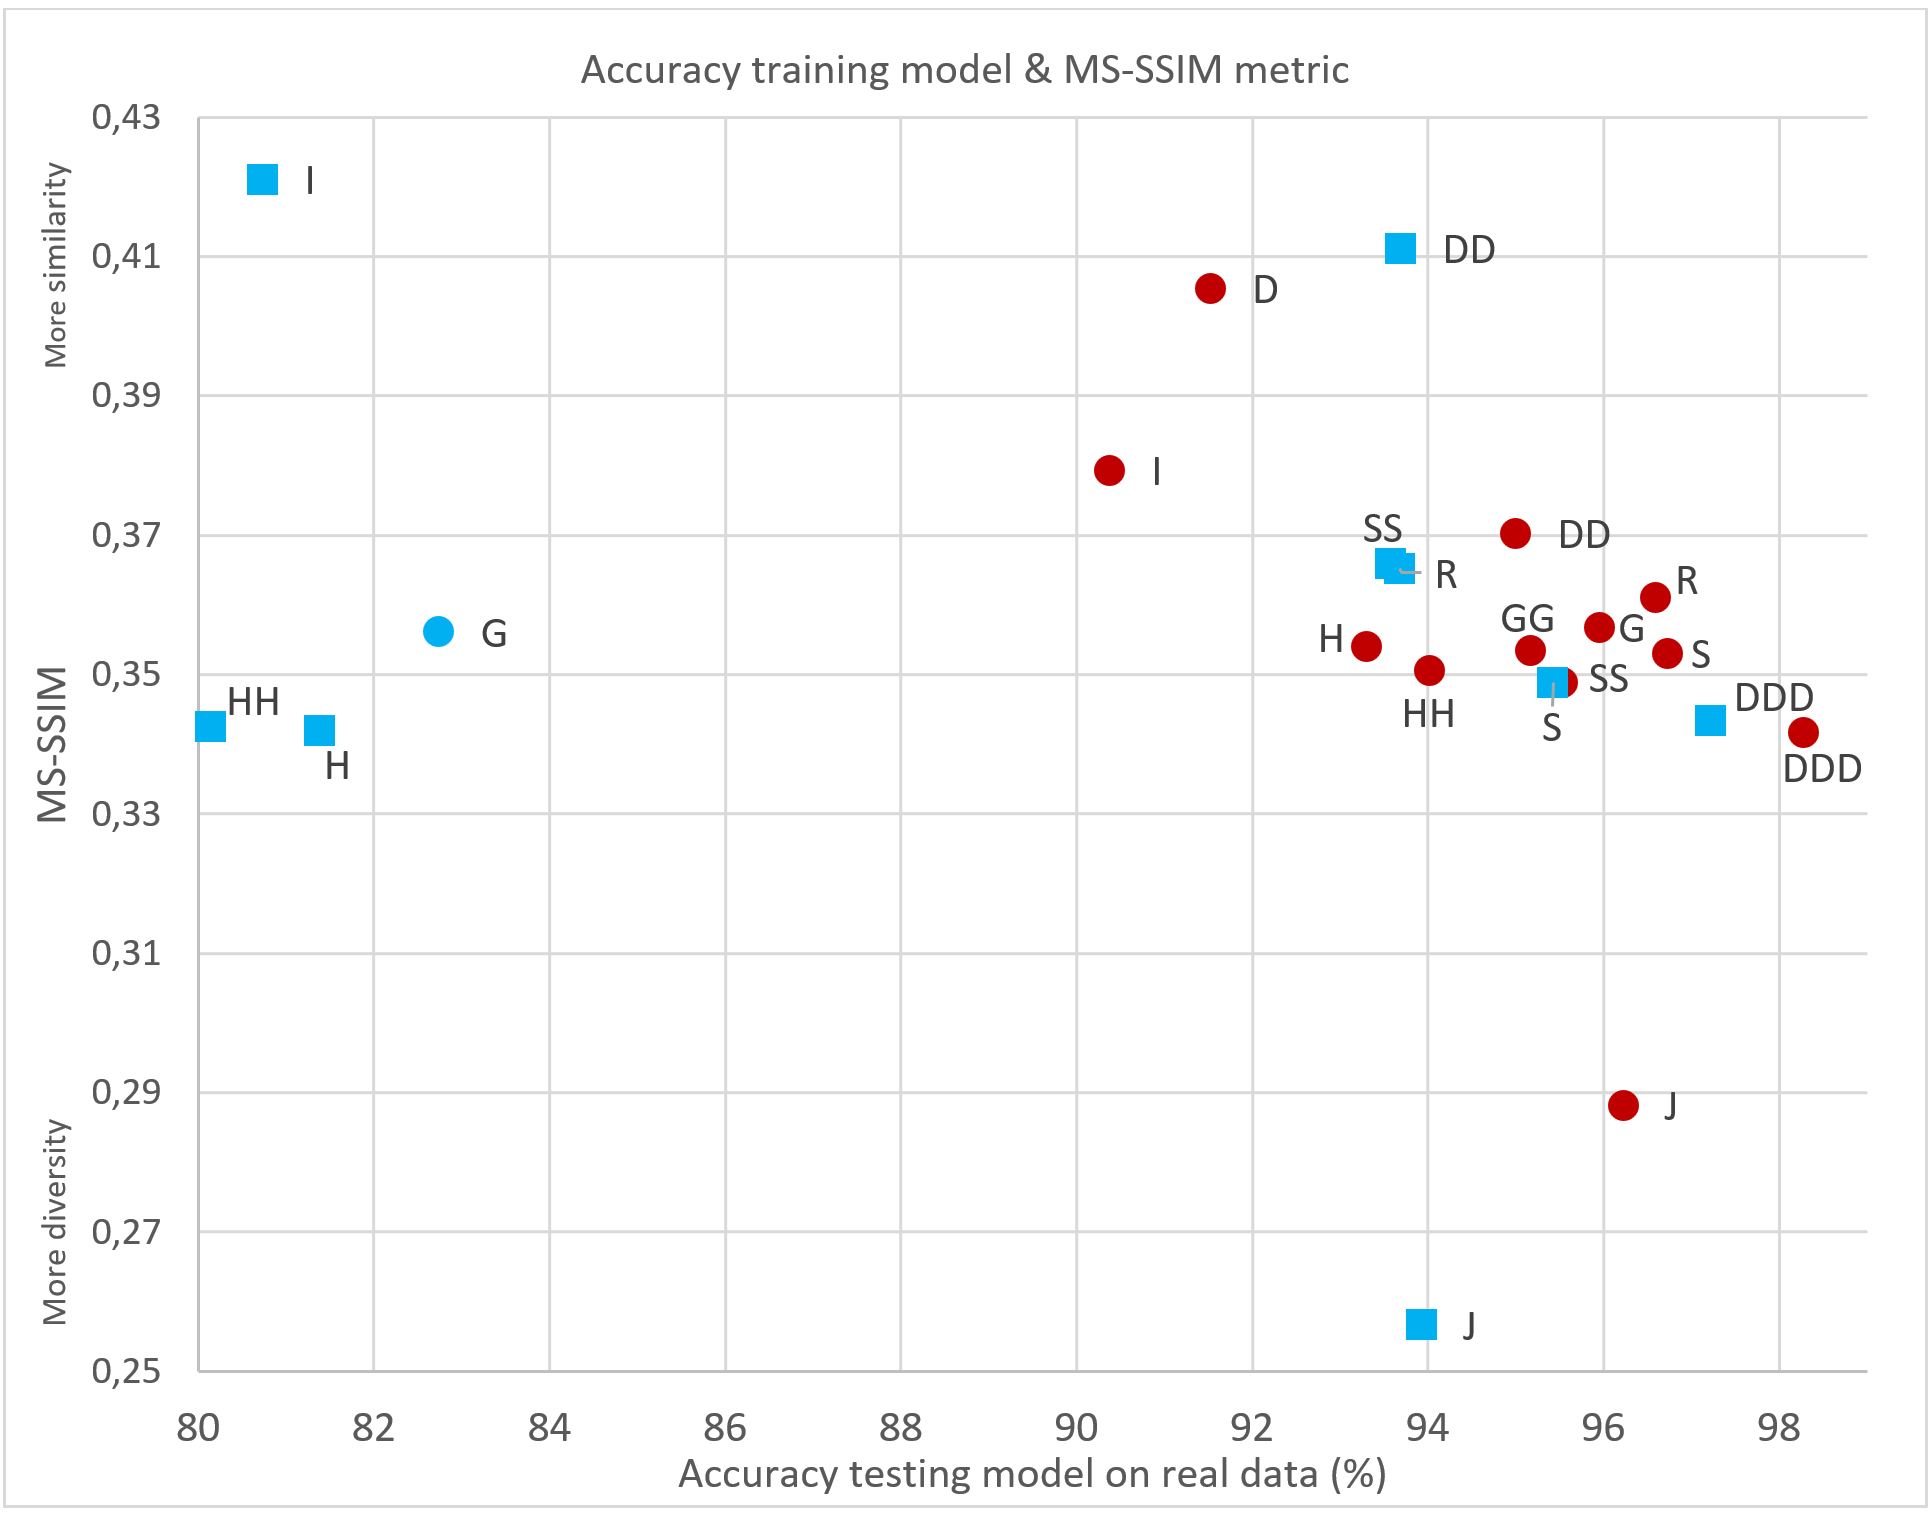
\includegraphics[width=0.7\textwidth,keepaspectratio]{img/prueba_msssim.png}}
\caption{Accuracy of model testing and MS-SSIM metric. \textcolor{dotgreen}{\textbf{Green}} shape indicates real dataset, \textcolor{dotred}{\textbf{red}} circles indicate datasets with real and augmented data, and \textcolor{dotsky}{\textbf{turquoise}} squares are entirely augmented datasets. The codes are described in Table \ref{table:code_dataset}.}
\label{fig:da_test_msssim}
\end{figure*}

\begin{figure*}
\centering
{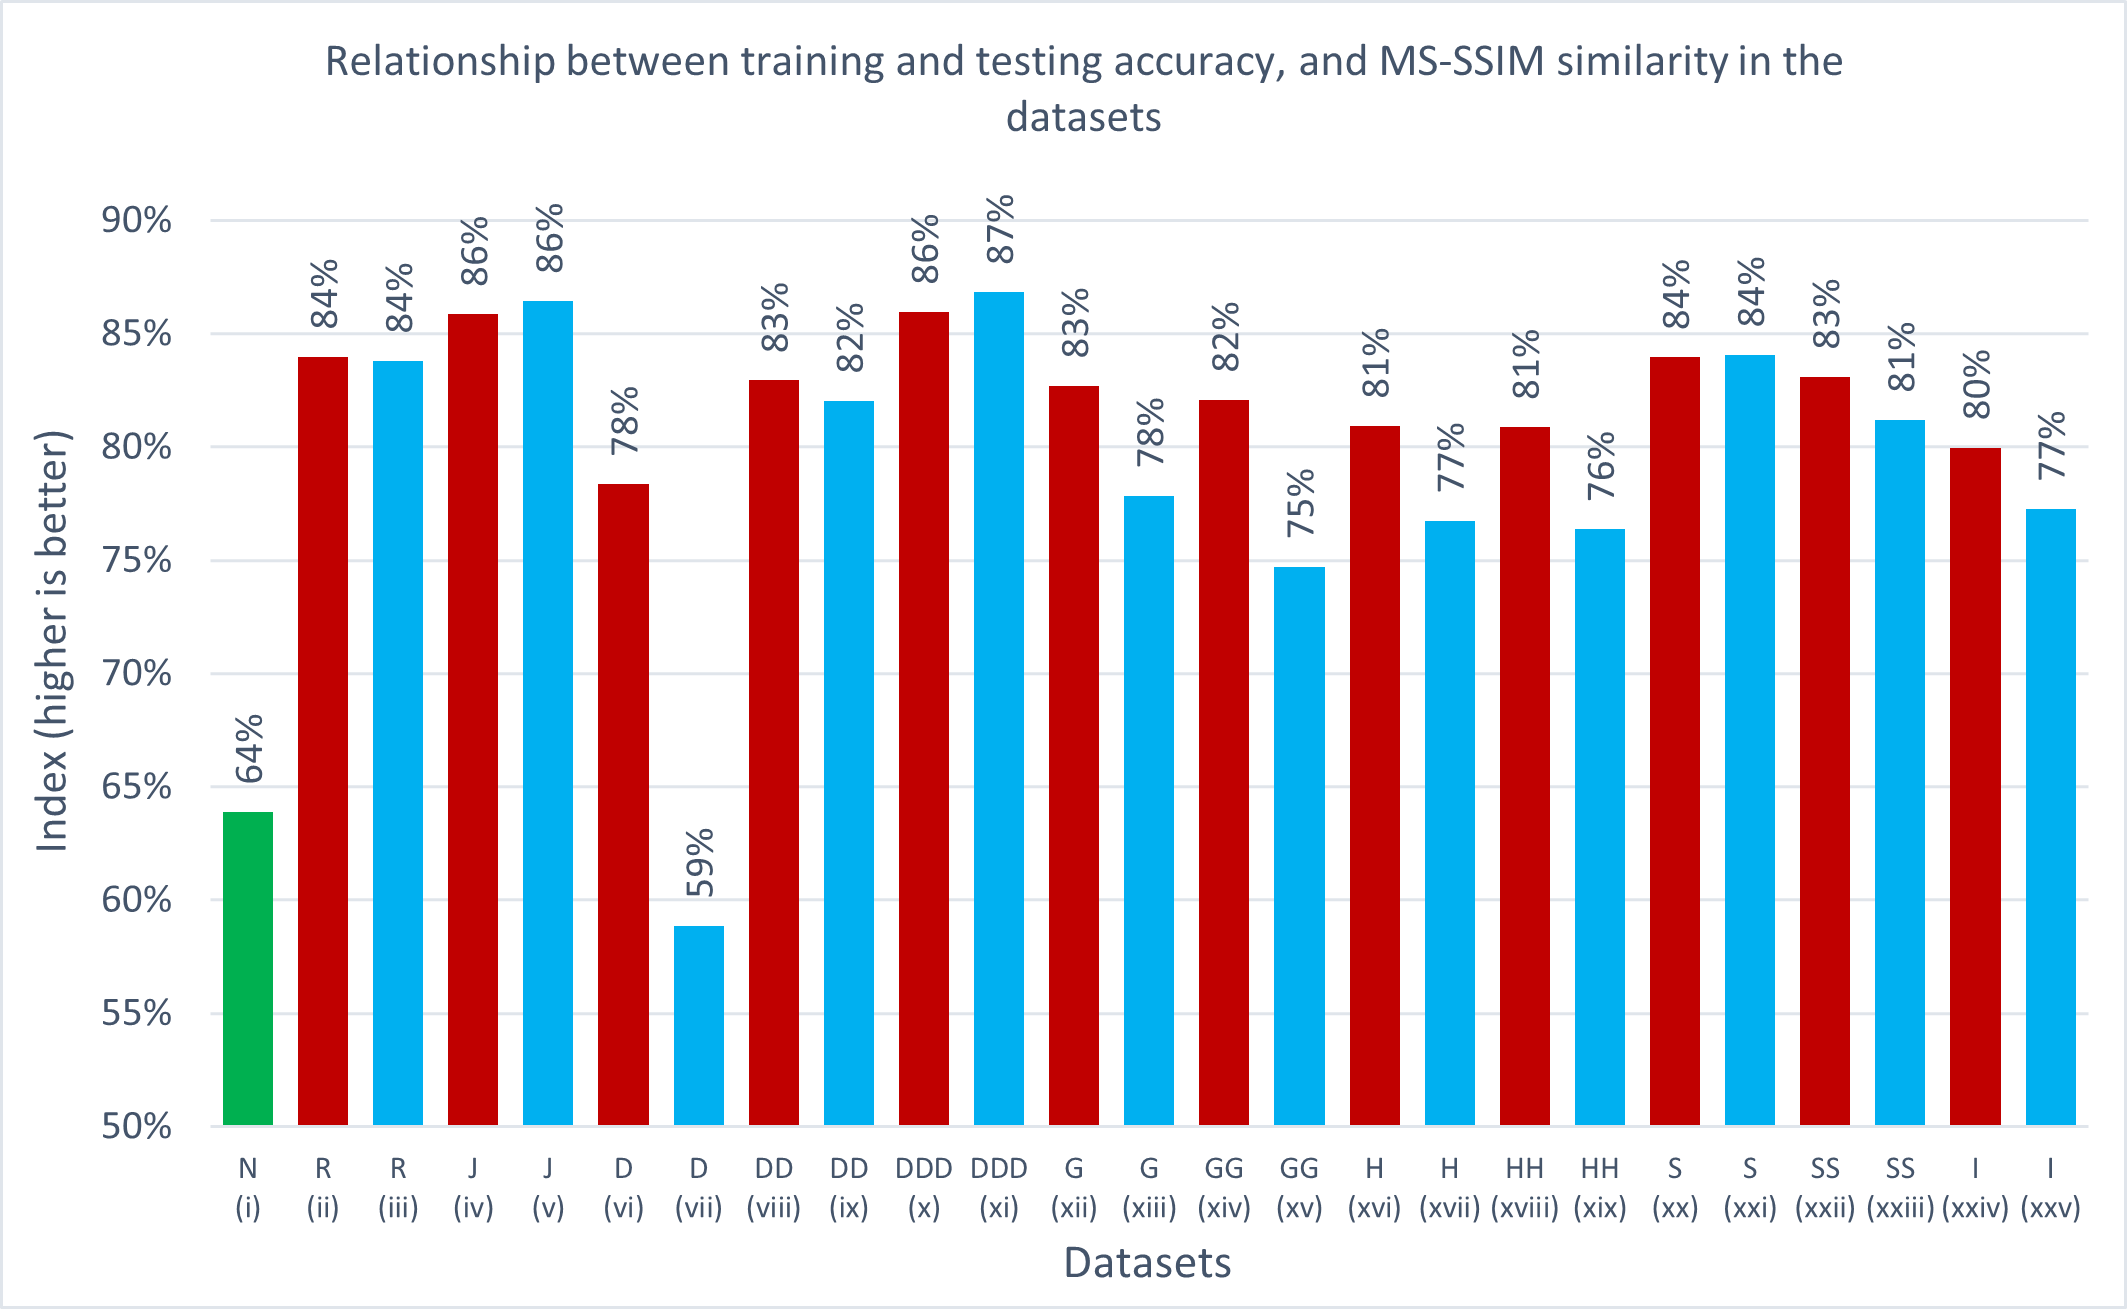
\includegraphics[width=0.7\textwidth,keepaspectratio]{img/relation_index.png}}
\caption{Index that relates model training accuracy (higher is better), model testing accuracy on real data (higher is better), and the value of the MS-SSIM metric (lower is better). \textcolor{dotgreen}{\textbf{Green}} shape indicates real dataset, \textcolor{dotred}{\textbf{red}} indicate datasets with real and augmented data, and \textcolor{dotsky}{\textbf{turquoise}} are entirely augmented datasets. The codes are described in Table \ref{table:code_dataset}.}
\label{fig:relation_index}
\end{figure*}

\section{Discussion}\label{discussion}
The various experiments conducted in this research highlight the performance of the probabilistic model on unbalanced datasets. Specifically, dataset (i) produced a model biased toward the LP, TC, and VT events, as shown in Table \ref{table:training_performance}.
The results indicate that balanced datasets yield higher-performing models, as they expand the examples within the event feature space. The models were subsequently tested on real data, demonstrating competitive classification levels in most cases. Transfer learning facilitated the development of deep learning models in a reduced timeframe, as evidenced in Table \ref{table:training_performance}.
In Tables \ref{table:training_performance} and \ref{table:testing_real_dataset}, it is evident that the drifting data augmentation technique achieved the best results across nearly all pre-trained models. This success may be attributed to the drifting technique's ability to effectively cover the data space. The most notable result is from drifting (xi), which, with a drift range of 0.0001-0.001, achieved an accuracy of 97.6\% over an entirely augmented dataset. An additional noteworthy result is the rotation (iii) technique, which, with a range of 5\%-25\%, achieved an accuracy of 94.2% on another augmented dataset.
In both cases, the F1 score metrics closely correspond to their respective accuracies. Although both models were derived from entirely augmented data, they performed well in real data tests, achieving accuracies of 97.2\% for (xi) and 93.7\% for (iii) (refer to Table \ref{table:testing_real_dataset}). However, the highest accuracy of 98.3\% was recorded for model (x), which utilized both real and augmented data.
It can be observed that the dataset composed of real and augmented data (x) generated by drifting in the range of 0.0001-0.001 reaches an accuracy of 93.8\%. Then the dataset of augmented data (ix) generated by drifting in range 0.001-0.01, reaches an accuracy of 93.5\%. Then we have the augmented data dataset (xxv) generated by Autoencoder Interpolation in the range 40\%-60\%, it obtains an accuracy of 93.1\% (Table \ref{table:training_performance}). These models also show good performance in tests with real data, with accuracies of 98.3\% for (x), 93.7\% for (ix) and 80.7\% for (xxv) (Table \ref{table:testing_real_dataset}). Only the last model (xxv) has a large distance between training and test accuracy on real data.
To obtain a generalized dataset, data from several stations were considered to generate a multi-station generalized probabilistic model. Furthermore, it was observed that models trained with completely augmented data achieved high recognition accuracy with real data in most cases (Table \ref{table:testing_real_dataset}).
Figure \ref{fig:da_training_test} shows that drifting, rotation, interpolation, specaugment and jittering have slightly better accuracy values than the other techniques. In general, the trained models perform better when tested on real data than during training. \\
Regarding the similarity and diversity metrics, it can be seen that the MS-SSIM values for the rotation and drifting techniques are similar, although the former shows more diversity, depending on the generation parameters (Table \ref{table:similarity_diversity_metrics}).
It can also be observed that Jittering exhibits higher diversity in datasets (v) and (iv), with MS-SSIM values of 0.26 and 0.29, respectively.
The dataset with the highest similarity and lowest diversity is Drifting (0.01-0.1) (vii), which has an MS-SSIM index of 0.78. This is followed by Interpolation (xxv) and Drifting (vi), with MS-SSIM values of 0.42 and 0.41, respectively.
Figure \ref{fig:da_training_msssim} illustrates the concentration of points representing the MS-SSIM similarity metric against the accuracy of model training. Notably, two distant points are evident: the dataset comprising only real data (i), which has low accuracy due to being unbalanced, and the drifting dataset (vii) with a range of 0.01-0.1, which shows higher similarity. Upon zooming into Figure \ref{fig:da_training_msssim_zoom}, it is clear that almost all datasets demonstrate similar levels of diversity, including the real dataset; however, the augmented Jittering dataset (v) shows greater diversity.
When comparing augmented datasets with real and augmented datasets within the same data augmentation (DA) method, it can be noted that augmented datasets exhibit more diversity and superior training performance, especially with Jittering, SpecAugment (xx, xxii), and Rotation.
In Figure \ref{fig:da_test_msssim}, certain augmented and real datasets demonstrate better diversity and testing accuracy values compared to their counterparts within the same DA method. Notable examples include Drifting (x, xi), Rotation (ii, iii), and SpecAugment (xxii, xxiii).
By generating a simple index that accounts for the model training accuracy (which is better when higher) and the MS-SSIM metric value (which is more favorable when lower, indicating greater diversity), we can observe (see Figure \ref{fig:relation_index}) that models trained on the Drifting (x, xi), Jittering (iv, v), SpecAugment (xx, xxii), and Rotation (ii, iii) datasets are more relevant in terms of model accuracy and dataset diversity. Conversely, models with low indices, such as the Drifting dataset (vii) and the real event dataset (i), are disadvantaged by their lower diversity and unbalanced nature, respectively.


% needed in second column of first page if using \IEEEpubid
%\IEEEpubidadjcol


% An example of a floating figure using the graphicx package.
% Note that \label must occur AFTER (or within) \caption.
% For figures, \caption should occur after the \includegraphics.
% Note that IEEEtran v1.7 and later has special internal code that
% is designed to preserve the operation of \label within \caption
% even when the captionsoff option is in effect. However, because
% of issues like this, it may be the safest practice to put all your
% \label just after \caption rather than within \caption{}.
%
% Reminder: the "draftcls" or "draftclsnofoot", not "draft", class
% option should be used if it is desired that the figures are to be
% displayed while in draft mode.
%
%\begin{figure}[!t]
%\centering
%\includegraphics[width=2.5in]{myfigure}
% where an .eps filename suffix will be assumed under latex,
% and a .pdf suffix will be assumed for pdflatex; or what has been declared
% via \DeclareGraphicsExtensions.
%\caption{Simulation results for the network.}
%\label{fig_sim}
%\end{figure}

% Note that IEEE typically puts floats only at the top, even when this
% results in a large percentage of a column being occupied by floats.


% An example of a double column floating figure using two subfigures.
% (The subfig.sty package must be loaded for this to work.)
% The subfigure \label commands are set within each subfloat command,
% and the \label for the overall figure must come after \caption.
% \hfil is used as a separator to get equal spacing.
% Watch out that the combined width of all the subfigures on a
% line do not exceed the text width or a line break will occur.
%
%\begin{figure*}[!t]
%\centering
%\subfloat[Case I]{\includegraphics[width=2.5in]{box}%
%\label{fig_first_case}}
%\hfil
%\subfloat[Case II]{\includegraphics[width=2.5in]{box}%
%\label{fig_second_case}}
%\caption{Simulation results for the network.}
%\label{fig_sim}
%\end{figure*}
%
% Note that often IEEE papers with subfigures do not employ subfigure
% captions (using the optional argument to \subfloat[]), but instead will
% reference/describe all of them (a), (b), etc., within the main caption.
% Be aware that for subfig.sty to generate the (a), (b), etc., subfigure
% labels, the optional argument to \subfloat must be present. If a
% subcaption is not desired, just leave its contents blank,
% e.g., \subfloat[].


% An example of a floating table. Note that, for IEEE style tables, the
% \caption command should come BEFORE the table and, given that table
% captions serve much like titles, are usually capitalized except for words
% such as a, an, and, as, at, but, by, for, in, nor, of, on, or, the, to
% and up, which are usually not capitalized unless they are the first or
% last word of the caption. Table text will default to \footnotesize as
% IEEE normally uses this smaller font for tables.
% The \label must come after \caption as always.
%
%\begin{table}[!t]
%% increase table row spacing, adjust to taste
%\renewcommand{\arraystretch}{1.3}
% if using array.sty, it might be a good idea to tweak the value of
% \extrarowheight as needed to properly center the text within the cells
%\caption{An Example of a Table}
%\label{table_example}
%\centering
%% Some packages, such as MDW tools, offer better commands for making tables
%% than the plain LaTeX2e tabular which is used here.
%\begin{tabular}{|c||c|}
%\hline
%One & Two\\
%\hline
%Three & Four\\
%\hline
%\end{tabular}
%\end{table}


% Note that the IEEE does not put floats in the very first column
% - or typically anywhere on the first page for that matter. Also,
% in-text middle ("here") positioning is typically not used, but it
% is allowed and encouraged for Computer Society conferences (but
% not Computer Society journals). Most IEEE journals/conferences use
% top floats exclusively.
% Note that, LaTeX2e, unlike IEEE journals/conferences, places
% footnotes above bottom floats. This can be corrected via the
% \fnbelowfloat command of the stfloats package.


\section{Conclusion}\label{conclusion}
In this work, several data augmentation techniques have been described, developed, and applied to seismic-volcanic signals. Initially, these techniques were employed to balance the datasets and subsequently to generate entirely augmented datasets. Deep learning classification models were then trained on these datasets, utilizing transfer learning with the pre-trained AlexNet model.
The performance of the trained classification models was evaluated, revealing that data augmentation techniques enhance model performance.
It was observed that the trained classification models, in conjunction with the considered data augmentation methods, are competitive with the baseline presented in previous research. Additionally, the following results were achieved:
\begin{itemize} 
\item The integration of data from multiple stations on the Lascar volcano facilitated the construction of more generalized probabilistic models, thereby mitigating biases associated with individual stations through various data augmentation techniques.
\item Data augmentation techniques significantly improve the performance metrics of deep learning models, as they enable the generation of additional examples within the feature space of volcanic seismic events.
\item Similarity and diversity metrics were considered to analyze these characteristics in the datasets generated by the various data augmentation techniques presented, in addition to the performance of the models.
\item Transfer learning significantly expedited the generation of deep learning models compared to training from scratch. 
\end{itemize}
The findings of this work can be used to improve the performance of deep learning models in seismic-volcanic signal recognition, considering the data augmentation techniques presented. Furthermore, the results indicate that models trained exclusively on augmented datasets show excellent performance when tested with real data, in addition to exhibiting diversity, which represents a substantial contribution to seismic-volcanic signal recognition.
A repository is available on GitHub for data verification at: \href{https://github.com/franznet/daseismicsignals}{\color{blue}https://github.com/franznet/daseismicsignals}.

\section{Future Work}\label{future_work}
Future research could focus on optimizing the parameters of existing data augmentation methods to improve model performance. Furthermore, evaluating the effectiveness of these techniques on different types of seismic events and with varying levels of noise would provide deeper insight into their applicability. \\
The index calculated to compare the models was defined with a $1/3$ ratio for each component. A hyperparameter could be defined to give sufficient weight to model performance, model testing on real data, and dataset diversity.\\
Finally, integrating these data augmentation strategies with other machine learning approaches, such as ensemble learning or reinforcement learning, could lead to the development of more robust and accurate models for seismic-volcanic signal recognition. 
A large dataset could be generated using various data augmentation techniques from different channels, stations, and volcanoes.

% if have a single appendix:
%\appendix[Proof of the Zonklar Equations]
% or
%\appendix  % for no appendix heading
% do not use \section anymore after \appendix, only \section*
% is possibly needed

% use appendices with more than one appendix
% then use \section to start each appendix
% you must declare a \section before using any
% \subsection or using \label (\appendices by itself
% starts a section numbered zero.)
%


% \appendices
% \section{Proof of the First Zonklar Equation}
% Appendix one text goes here.

% you can choose not to have a title for an appendix
% if you want by leaving the argument blank
% \section{}
% Appendix two text goes here.


% use section* for acknowledgment
% \section*{Acknowledgment}
% The authors would like to thank...


% Can use something like this to put references on a page
% by themselves when using endfloat and the captionsoff option.
\ifCLASSOPTIONcaptionsoff
  \newpage
\fi



% trigger a \newpage just before the given reference
% number - used to balance the columns on the last page
% adjust value as needed - may need to be readjusted if
% the document is modified later
%\IEEEtriggeratref{8}
% The "triggered" command can be changed if desired:
%\IEEEtriggercmd{\enlargethispage{-5in}}

% references section

% can use a bibliography generated by BibTeX as a .bbl file
% BibTeX documentation can be easily obtained at:
% http://www.ctan.org/tex-archive/biblio/bibtex/contrib/doc/
% The IEEEtran BibTeX style support page is at:
% http://www.michaelshell.org/tex/ieeetran/bibtex/
%\bibliographystyle{IEEEtran}
% argument is your BibTeX string definitions and bibliography database(s)
%\bibliography{IEEEabrv,../bib/paper}
%
% <OR> manually copy in the resultant .bbl file
% set second argument of \begin to the number of references
% (used to reserve space for the reference number labels box)
%\begin{thebibliography}{1}
%\bibitem{IEEEhowto:kopka}
%H.~Kopka and P.~W. Daly, \emph{A Guide to \LaTeX}, 3rd~ed.\hskip 1em plus
%  0.5em minus 0.4em\relax Harlow, England: Addison-Wesley, 1999.
%\end{thebibliography}
\printbibliography



% biography section
%
% If you have an EPS/PDF photo (graphicx package needed) extra braces are
% needed around the contents of the optional argument to biography to prevent
% the LaTeX parser from getting confused when it sees the complicated
% \includegraphics command within an optional argument. (You could create
% your own custom macro containing the \includegraphics command to make things
% simpler here.)
\begin{IEEEbiography}[{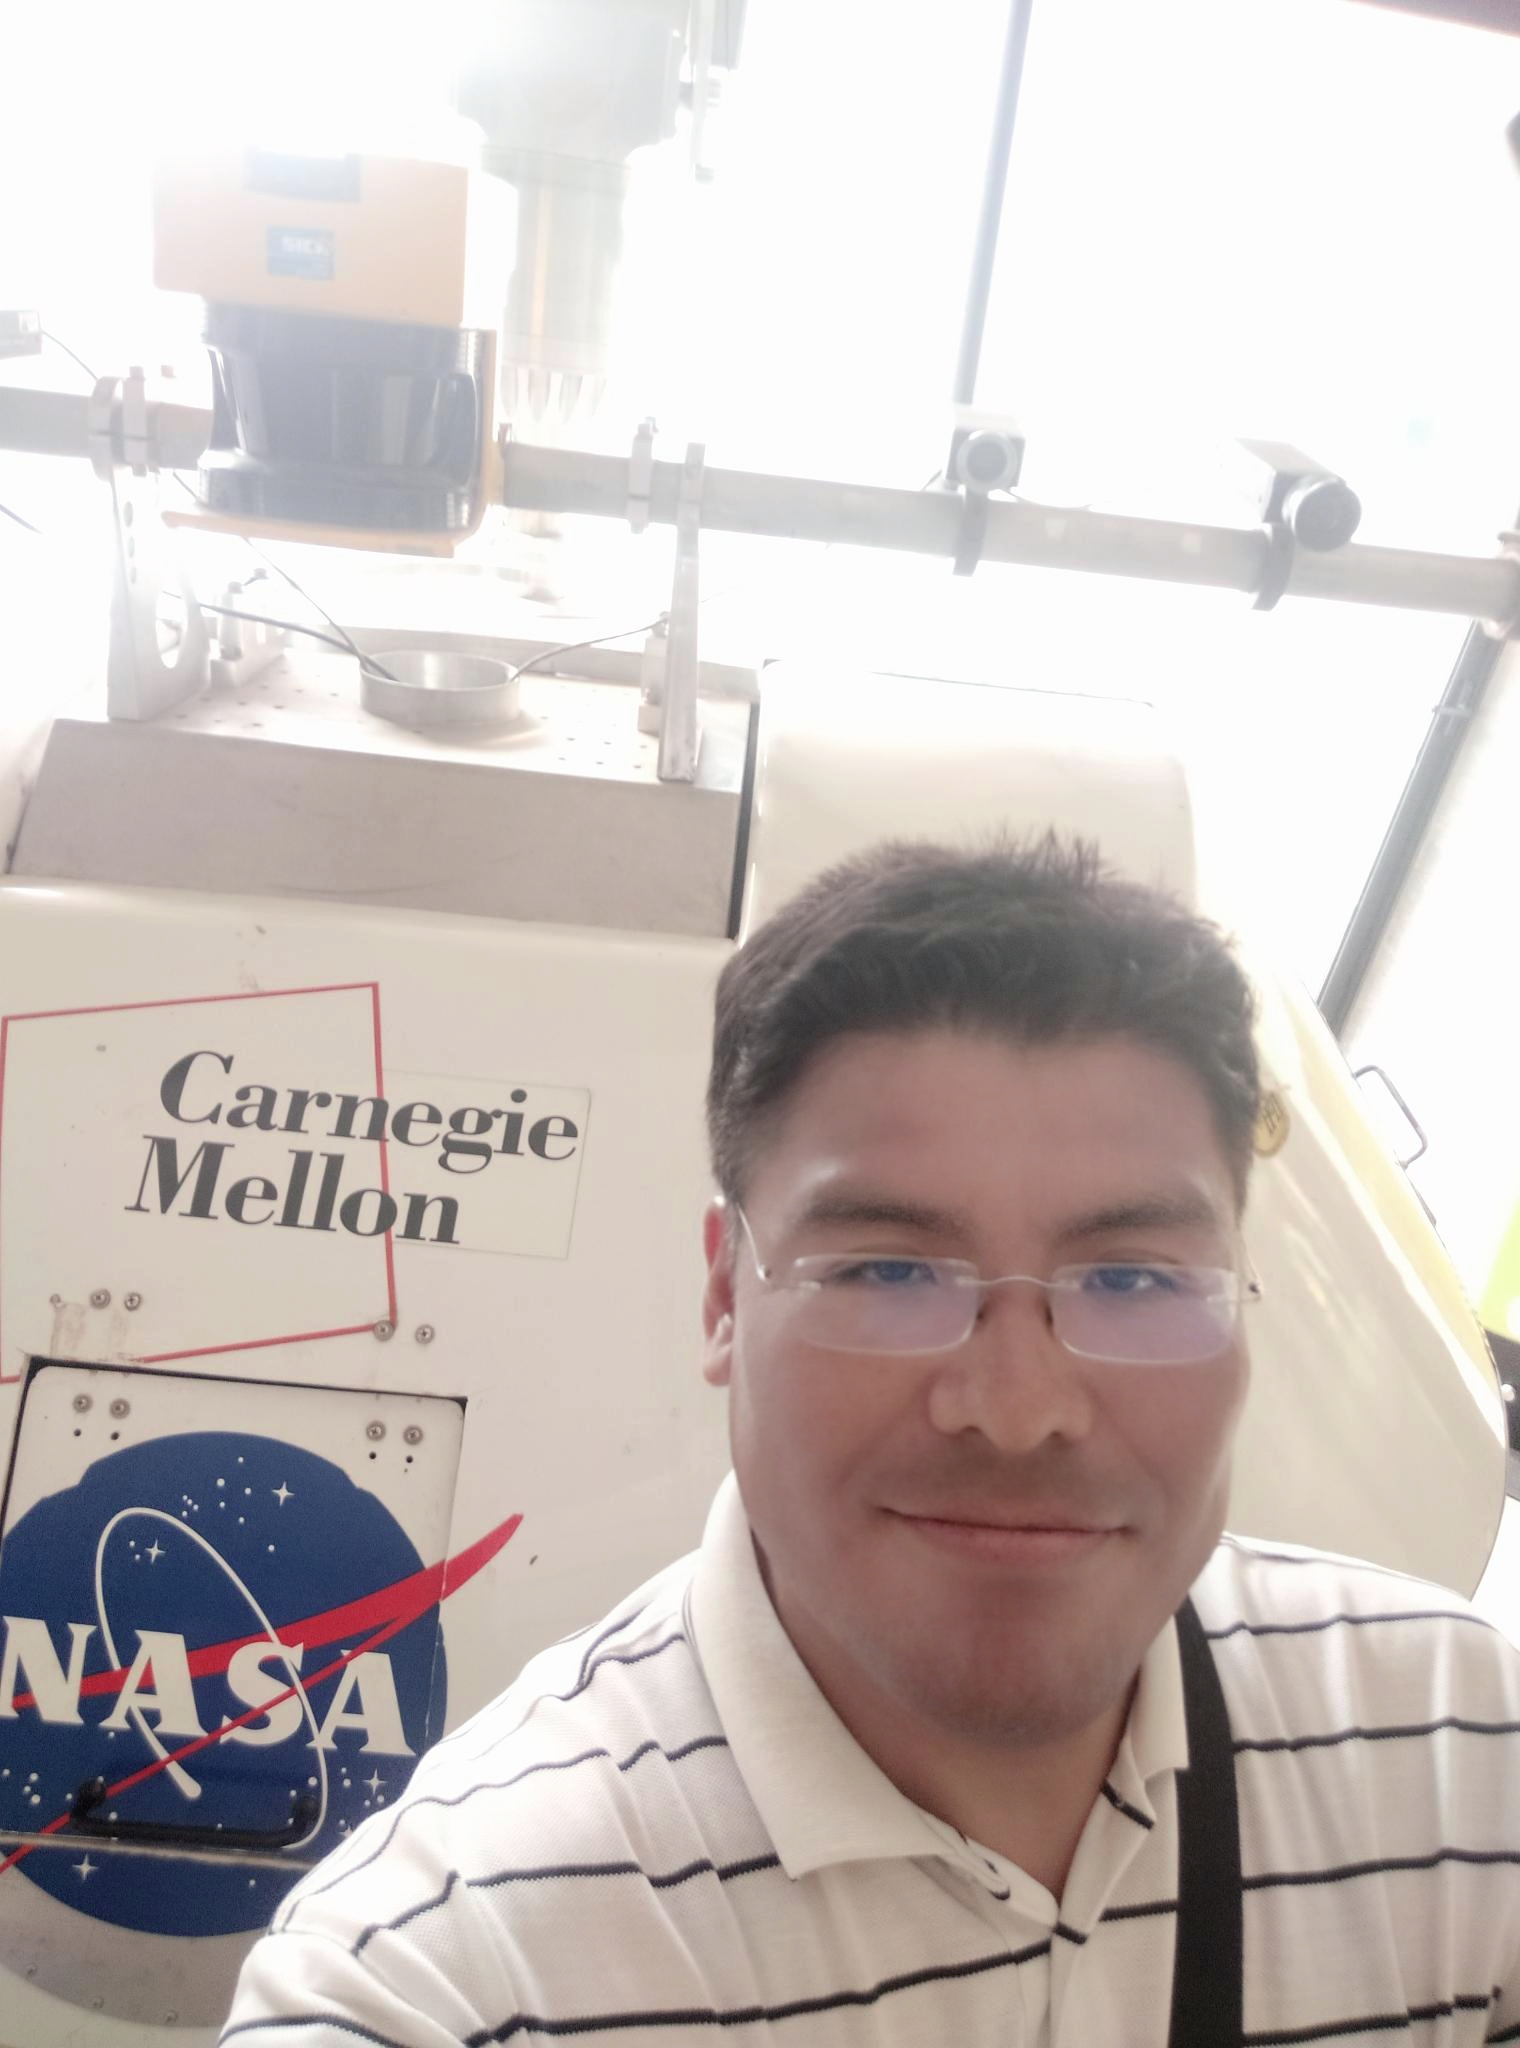
\includegraphics[width=1in,height=1.25in,clip,keepaspectratio]{img/franz.jpg}}]{Franz~Yupanqui~Machaca}
% or if you just want to reserve a space for a photo:
earned his Master's degree in Computer Engineering from the Universidad Católica del Norte in Chile in 2023. He is currently pursuing his Ph.D. in Sustainable Engineering at the Universidad Católica del Norte, focusing on the development of advanced algorithms for seismic-volcanic signal recognition. His research interests include deep learning techniques, transfer learning, data augmentation, computational intelligence in signals, data analytics, and more.
\end{IEEEbiography}

\begin{IEEEbiography}[{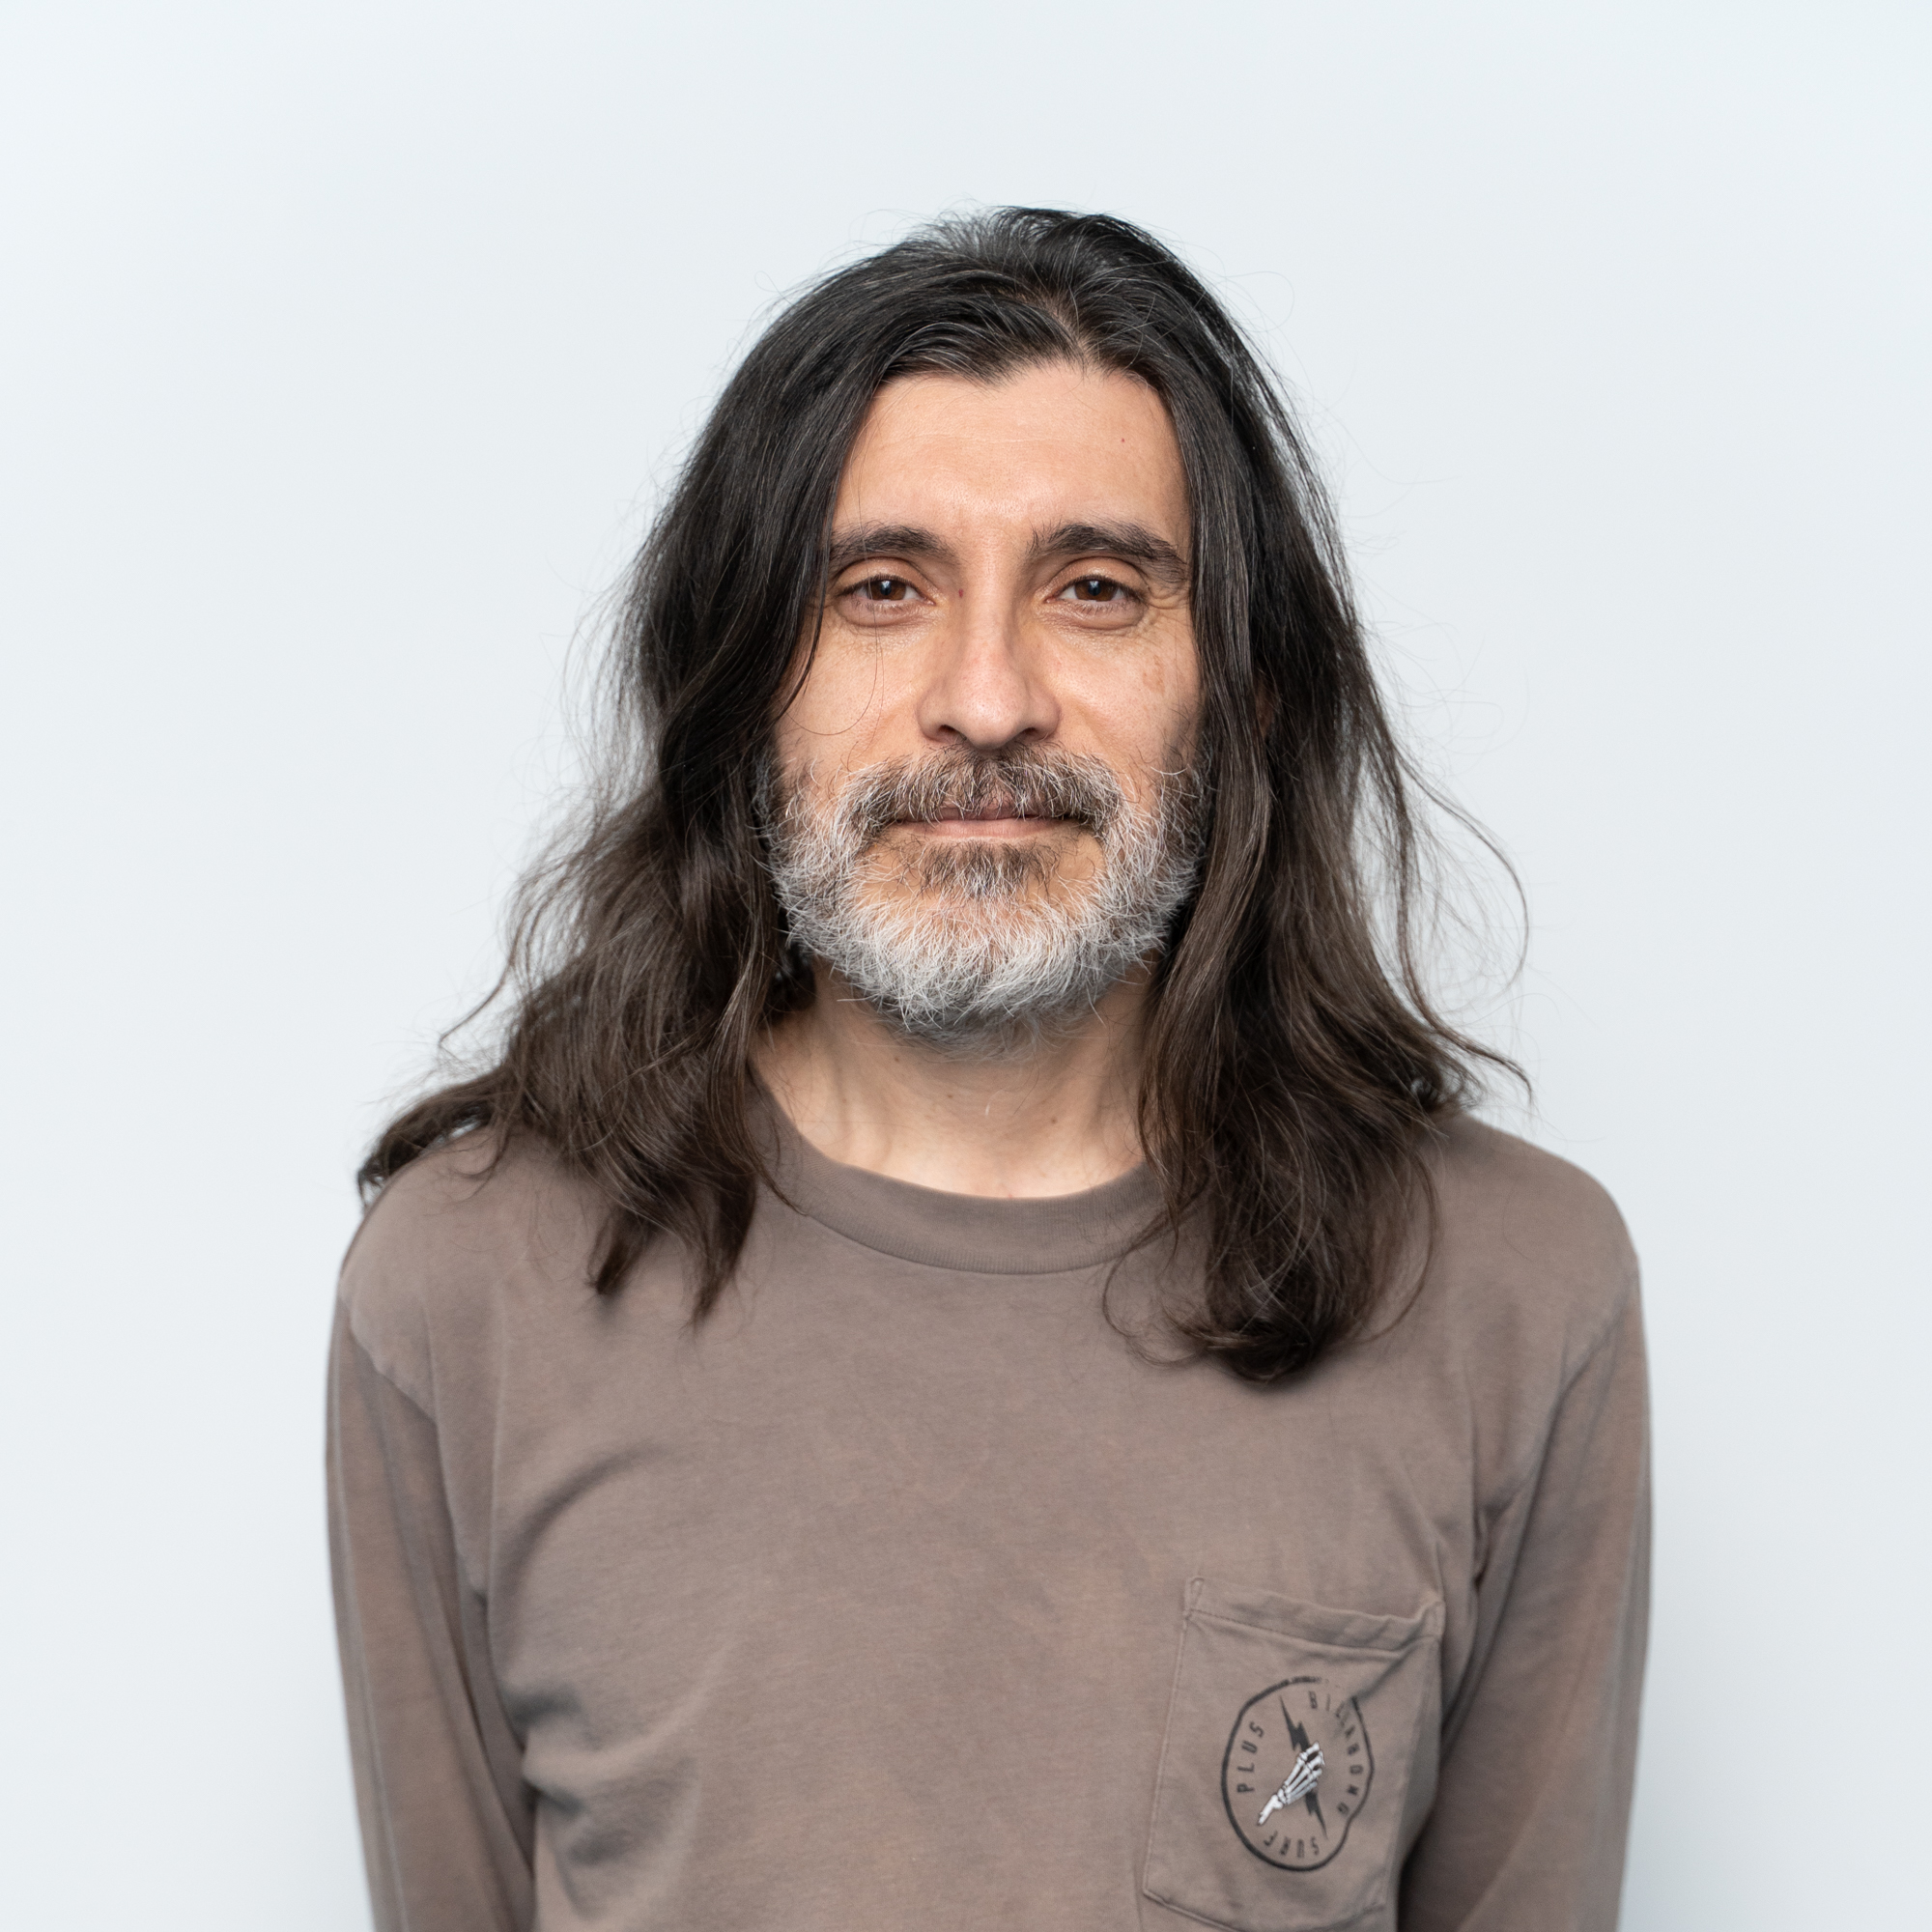
\includegraphics[width=1in,height=1.25in,clip,keepaspectratio]{img/pablo.jpg}}]{Pablo~Salazar~Reinoso}
received his Doktors der naturwissenschaften (Dr. Rer. Nat.) from the Free University of Berlin, Germany. Currently, he is Professor with the Department of Geological Sciences, Universidad Católica del Norte, Chile. His research interests include Remote Sensing, Automatic Control, Modeling, Seismotectonics, Microseismicity, Tectonics, Neotectonics, and more.
\end{IEEEbiography}

\begin{IEEEbiography}[{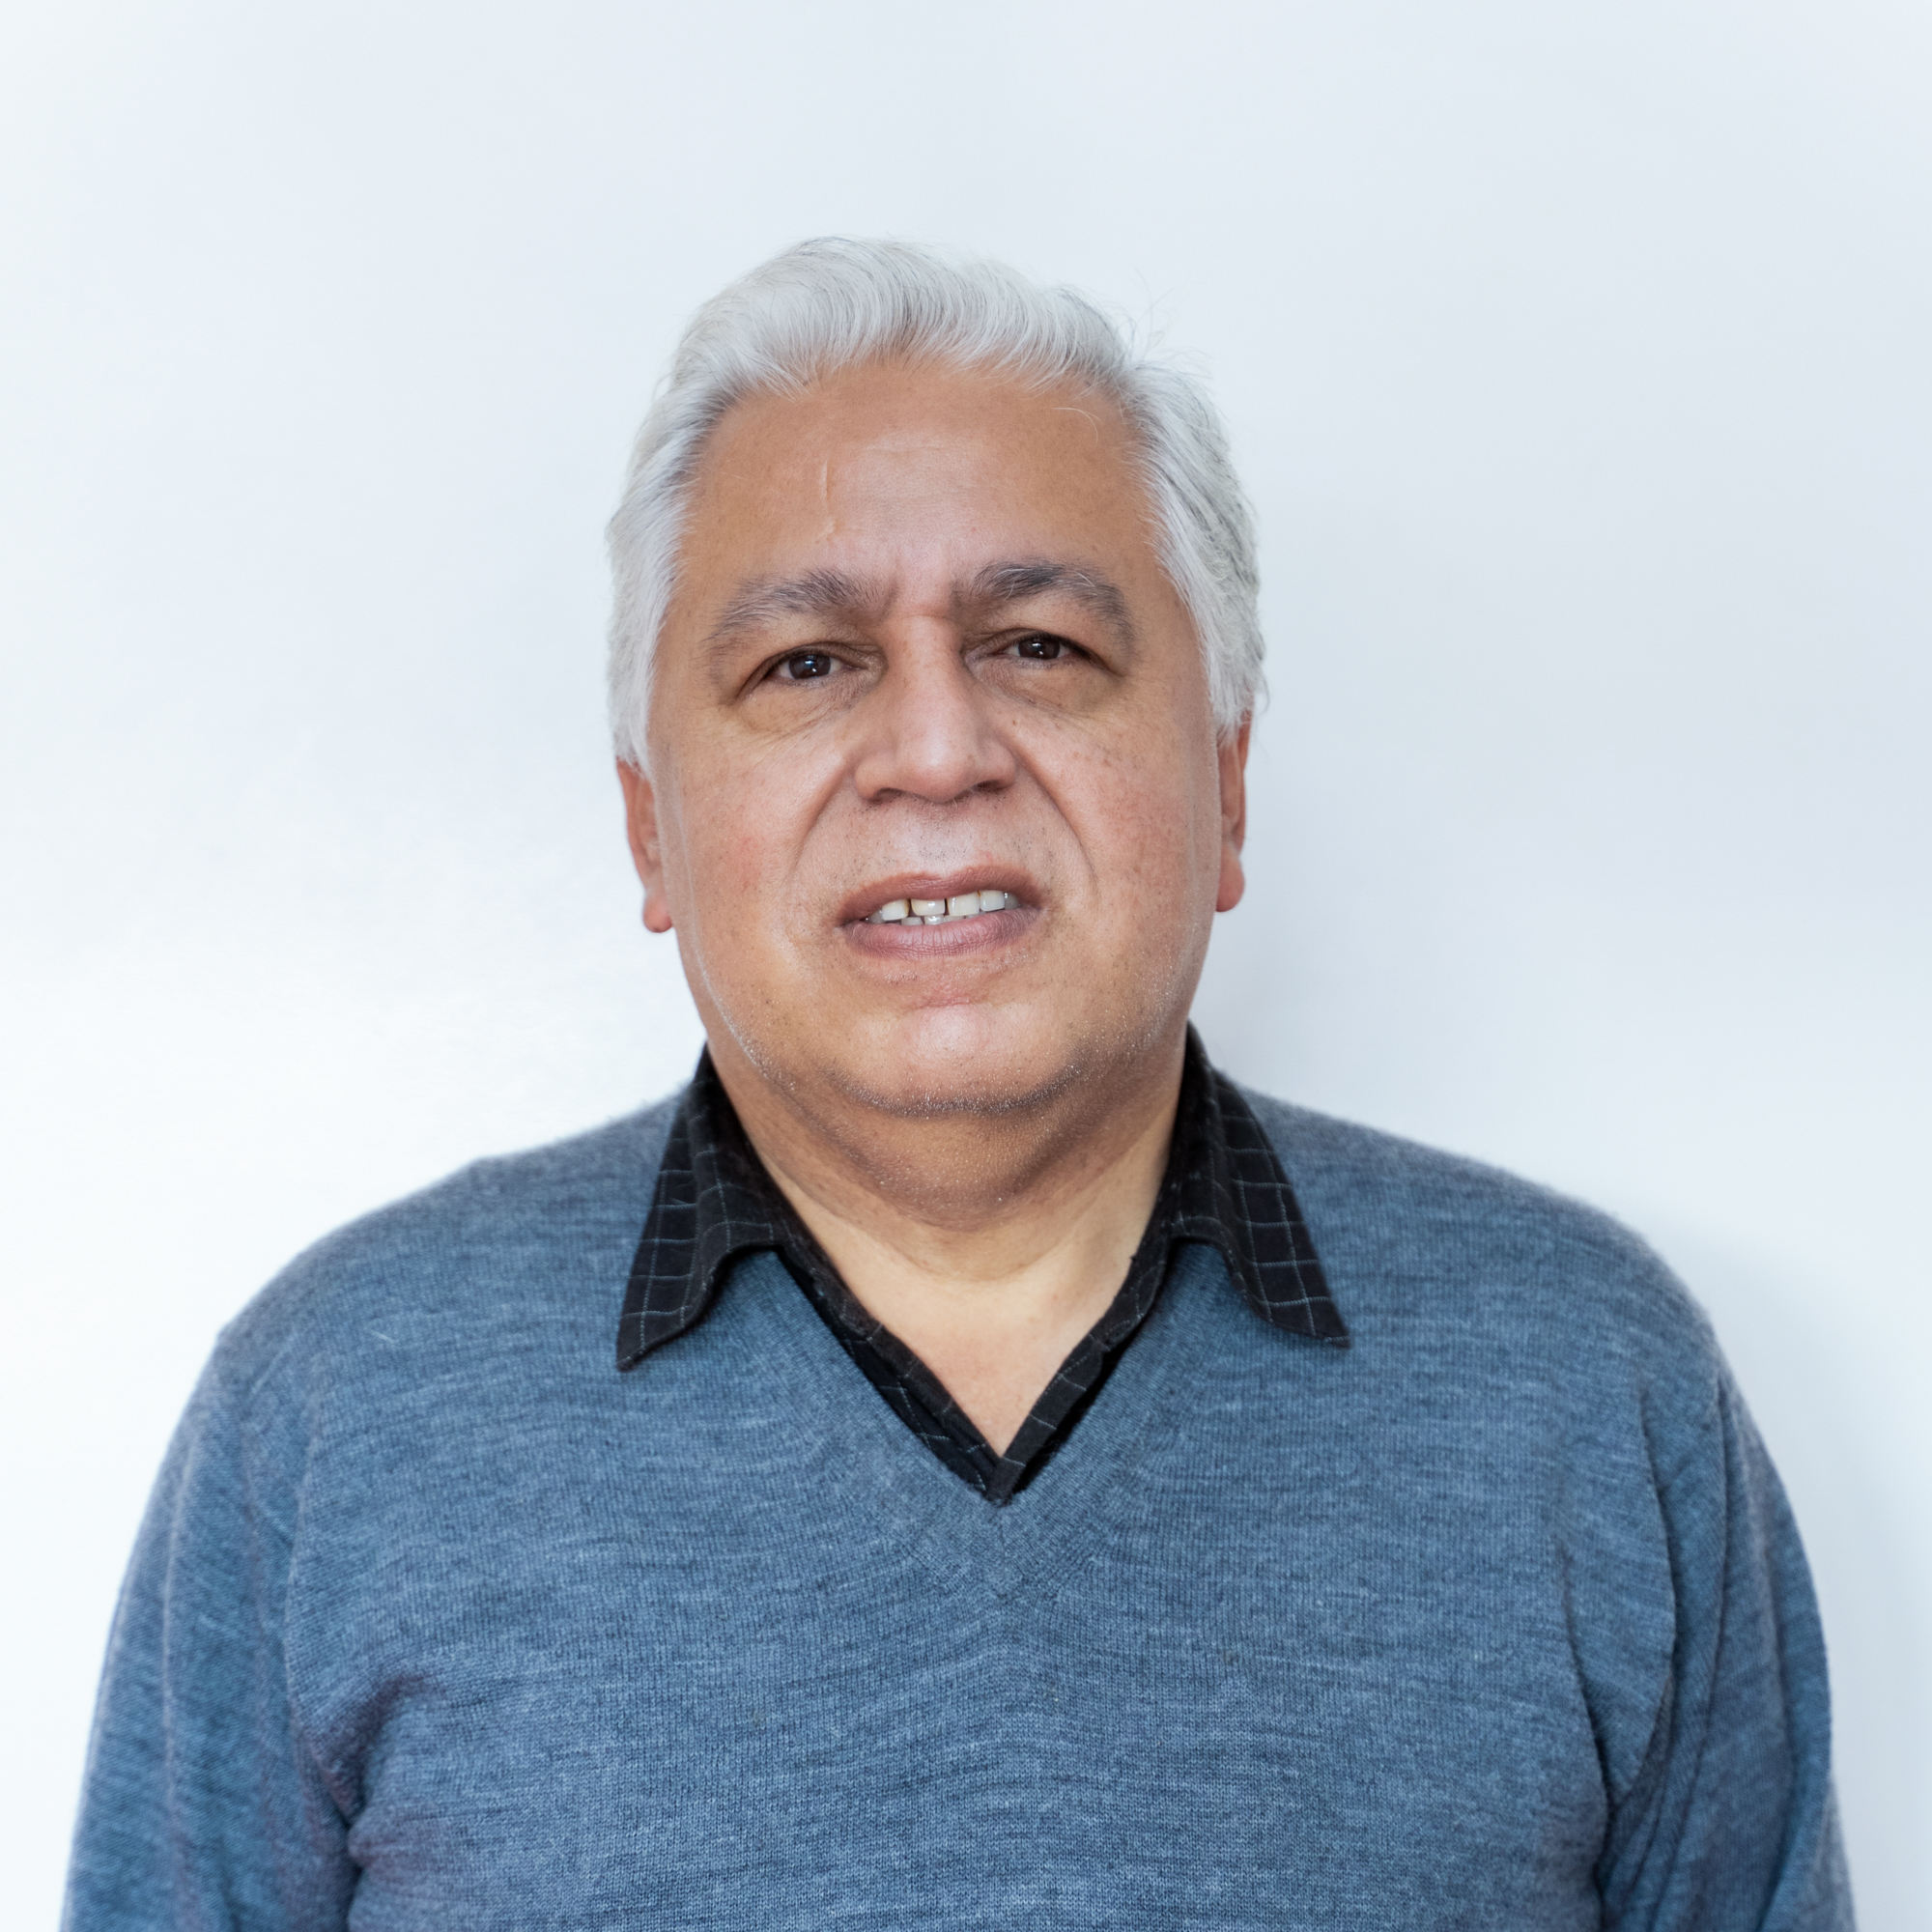
\includegraphics[width=1in,height=1.25in,clip,keepaspectratio]{img/claudio.jpg}}]{Claudio~Meneses~Villegas}
received his Ph.D. degree in Computer Science from the University of Massachusetts, EE.UU.. Currently, he is Professor with the Department of Computing and Systems Engineering, Universidad Católica del Norte, Chile. His research interests include Data Mining, Machine Learning, Data Visualization, Data Science, and more.
\end{IEEEbiography}

% You can push biographies down or up by placing
% a \vfill before or after them. The appropriate
% use of \vfill depends on what kind of text is
% on the last page and whether or not the columns
% are being equalized.

%\vfill

% Can be used to pull up biographies so that the bottom of the last one
% is flush with the other column.
%\enlargethispage{-5in}



% that's all folks
\end{document}
\begin{IEEEbiographynophoto}{John Doe}
Biography text here.
\end{IEEEbiographynophoto}

% insert where needed to balance the two columns on the last page with
% biographies
%\newpage

\begin{IEEEbiographynophoto}{Jane Doe}
Biography text here.
\end{IEEEbiographynophoto}

% You can push biographies down or up by placing
% a \vfill before or after them. The appropriate
% use of \vfill depends on what kind of text is
% on the last page and whether or not the columns
% are being equalized.

%\vfill

% Can be used to pull up biographies so that the bottom of the last one
% is flush with the other column.
%\enlargethispage{-5in}



% that's all folks
\end{document}